\documentclass[11pt]{article} 

%\documentclass[paper=a4,fontsize=11pt]{scrartcl}	 			% KOMA-article class
							
%\usepackage[english]{babel}								% English language/hyphenation
%\usepackage[protrusion=true,expansion=true]{microtype}		% Better typography
\usepackage{amsmath,amsfonts,amsthm}					% Math packages
\usepackage[pdftex]{graphicx}								% Enable pdflatex
\usepackage[svgnames]{xcolor}							% Colors by their 'svgnames'
\usepackage{geometry}
	\textheight=700px									% Saving trees ;-) 
\usepackage{url}										% Clickable URL's
\usepackage{wrapfig}									% Wrap text along figures


\frenchspacing									% Better looking spacings after periods
%\pagestyle{empty}								% No pagenumbers/headers/footers
%\usepackage{bbding}									% Symbols


% ------- Enable UTF8 characters ------- %
%\usepackage[utf8]{inputenc}
\usepackage[english]{babel}

\usepackage[colorinlistoftodos,prependcaption,textsize=normal]{todonotes}

\usepackage{listings}
\usepackage{color}

%\usepackage{pdfpages}

% ------------ Code Listing ------------- %

\definecolor{dkgreen}{rgb}{0,0.6,0}
\definecolor{gray}{rgb}{0.5,0.5,0.5}
\definecolor{mauve}{rgb}{0.58,0,0.82}

\lstset{frame=false,
  language=C++,
  aboveskip=3mm,
  belowskip=3mm,
  showstringspaces=false,
  columns=flexible,
  basicstyle={\small\ttfamily},
  numbers=none,
  numberstyle=\tiny\color{gray},
  keywordstyle=\color{blue},
  commentstyle=\color{dkgreen},
  stringstyle=\color{mauve},
  breaklines=true,
  breakatwhitespace=true,
  tabsize=3,
  moredelim=**[is][\color{mauve}]{@}{@},
}

% ------- Page layout ------- %
\usepackage{fullpage}
\usepackage{hyperref} % clickable references
\hypersetup{
    colorlinks,
    citecolor=black,
    filecolor=black,
    linkcolor=black,
    urlcolor=black
}
\usepackage{multicol}
\setlength{\columnsep}{1cm}

\setlength\parindent{0pt}

% ------- Images ------- %
\usepackage{graphicx}
\usepackage{caption}
\usepackage{float}
\usepackage{subcaption}
\DeclareCaptionFont{gray}{\color{gray}}
\captionsetup{textfont={footnotesize,sc,gray},font={footnotesize,sc,gray}}
\usepackage{blindtext}

% Test

\usepackage{tikz}
\usetikzlibrary{shapes,arrows,shadows}
\newcommand{\mx}[1]{\mathbf{\bm{#1}}} % Matrix command
\newcommand{\vc}[1]{\mathbf{\bm{#1}}} % Vector command

\usetikzlibrary{arrows}


\title{Elektriske Maskiner}


\begin{document}

\begin{titlepage}
\begin{center}


\textsc{\LARGE University of Southern Denmark}\\[1.5cm]
\textsc{\Large Introduction to Robotics and Computer Vision}\\[0.5cm]
\vfill
\hrule ~\\[0.3cm]
{ \huge \bfseries Vision -- Mandatory Exercise 1\\ Image restoration\\[0.4cm] }
\hrule ~\\[1.5cm]
\vfill

% Author and supervisor
\begin{minipage}[t]{7.9cm}
\begin{flushleft} \large
\emph{by:}\\
Keerthikan Ratnarajah  \\
kerat12@student.sdu.dk \\
Jes Grydholdt Jepsen   \\
jejep12@student.sdu.dk 
\end{flushleft}
\end{minipage}
\begin{minipage}[t]{7.9cm}
\begin{flushright} \large

\end{flushright}
\end{minipage}

\vspace{1.2cm}
Dato: \today


\end{center}
\end{titlepage}

\listoftodos
\tableofcontents

\newpage
\section{Introduction}
In the real world images are sometimes affected by noise in a way that makes working with them (or looking at them) difficult. The purpose of this project is therefore look at image restoration on a set of images that are affected by different kinds of defects. The overall task is to minimize the impact of the noise and thereby to improve the quality of the image.\\[0.2cm]
To come up with an analysis and a way to remove (or weaken) the defect, the following considerations are done for each image: 
\begin{itemize}\itemsep-3pt
\item Investigate the image and identify the defect, for example by using the histogram and/or the frequency spectrum of the image.
\item Design a solution that removes or weakens the impact of the defect and investigate the properties of the solution. 
\item Investigate different solution possibilities.
\item Implement and apply the solution(s)
\end{itemize}



\section{Image 1}
Figure \ref{fig:img1_src} shows the original image, This image is compared to the original much darker.  Based on the histogram taken from the image it can be seen that a high amount of black pixels in the image. This form of noise is usually called a pepper noise, at which an image is infected w

\section{Image 2 -- Salt and Pepper noise}
Figure \ref{fig:img2_src} shows the original image, which is filled with black and white pixels. This kind of noise is known as salt--and--pepper noise, and from the histogram of the image (figure \ref{fig:img2_hist}) can the amount of salt--and--pepper noise be seen; salt noise on the right and pepper noise on the left. 
\begin{figure}[H]
    \centering
    \begin{subfigure}[b]{0.23\textwidth}
        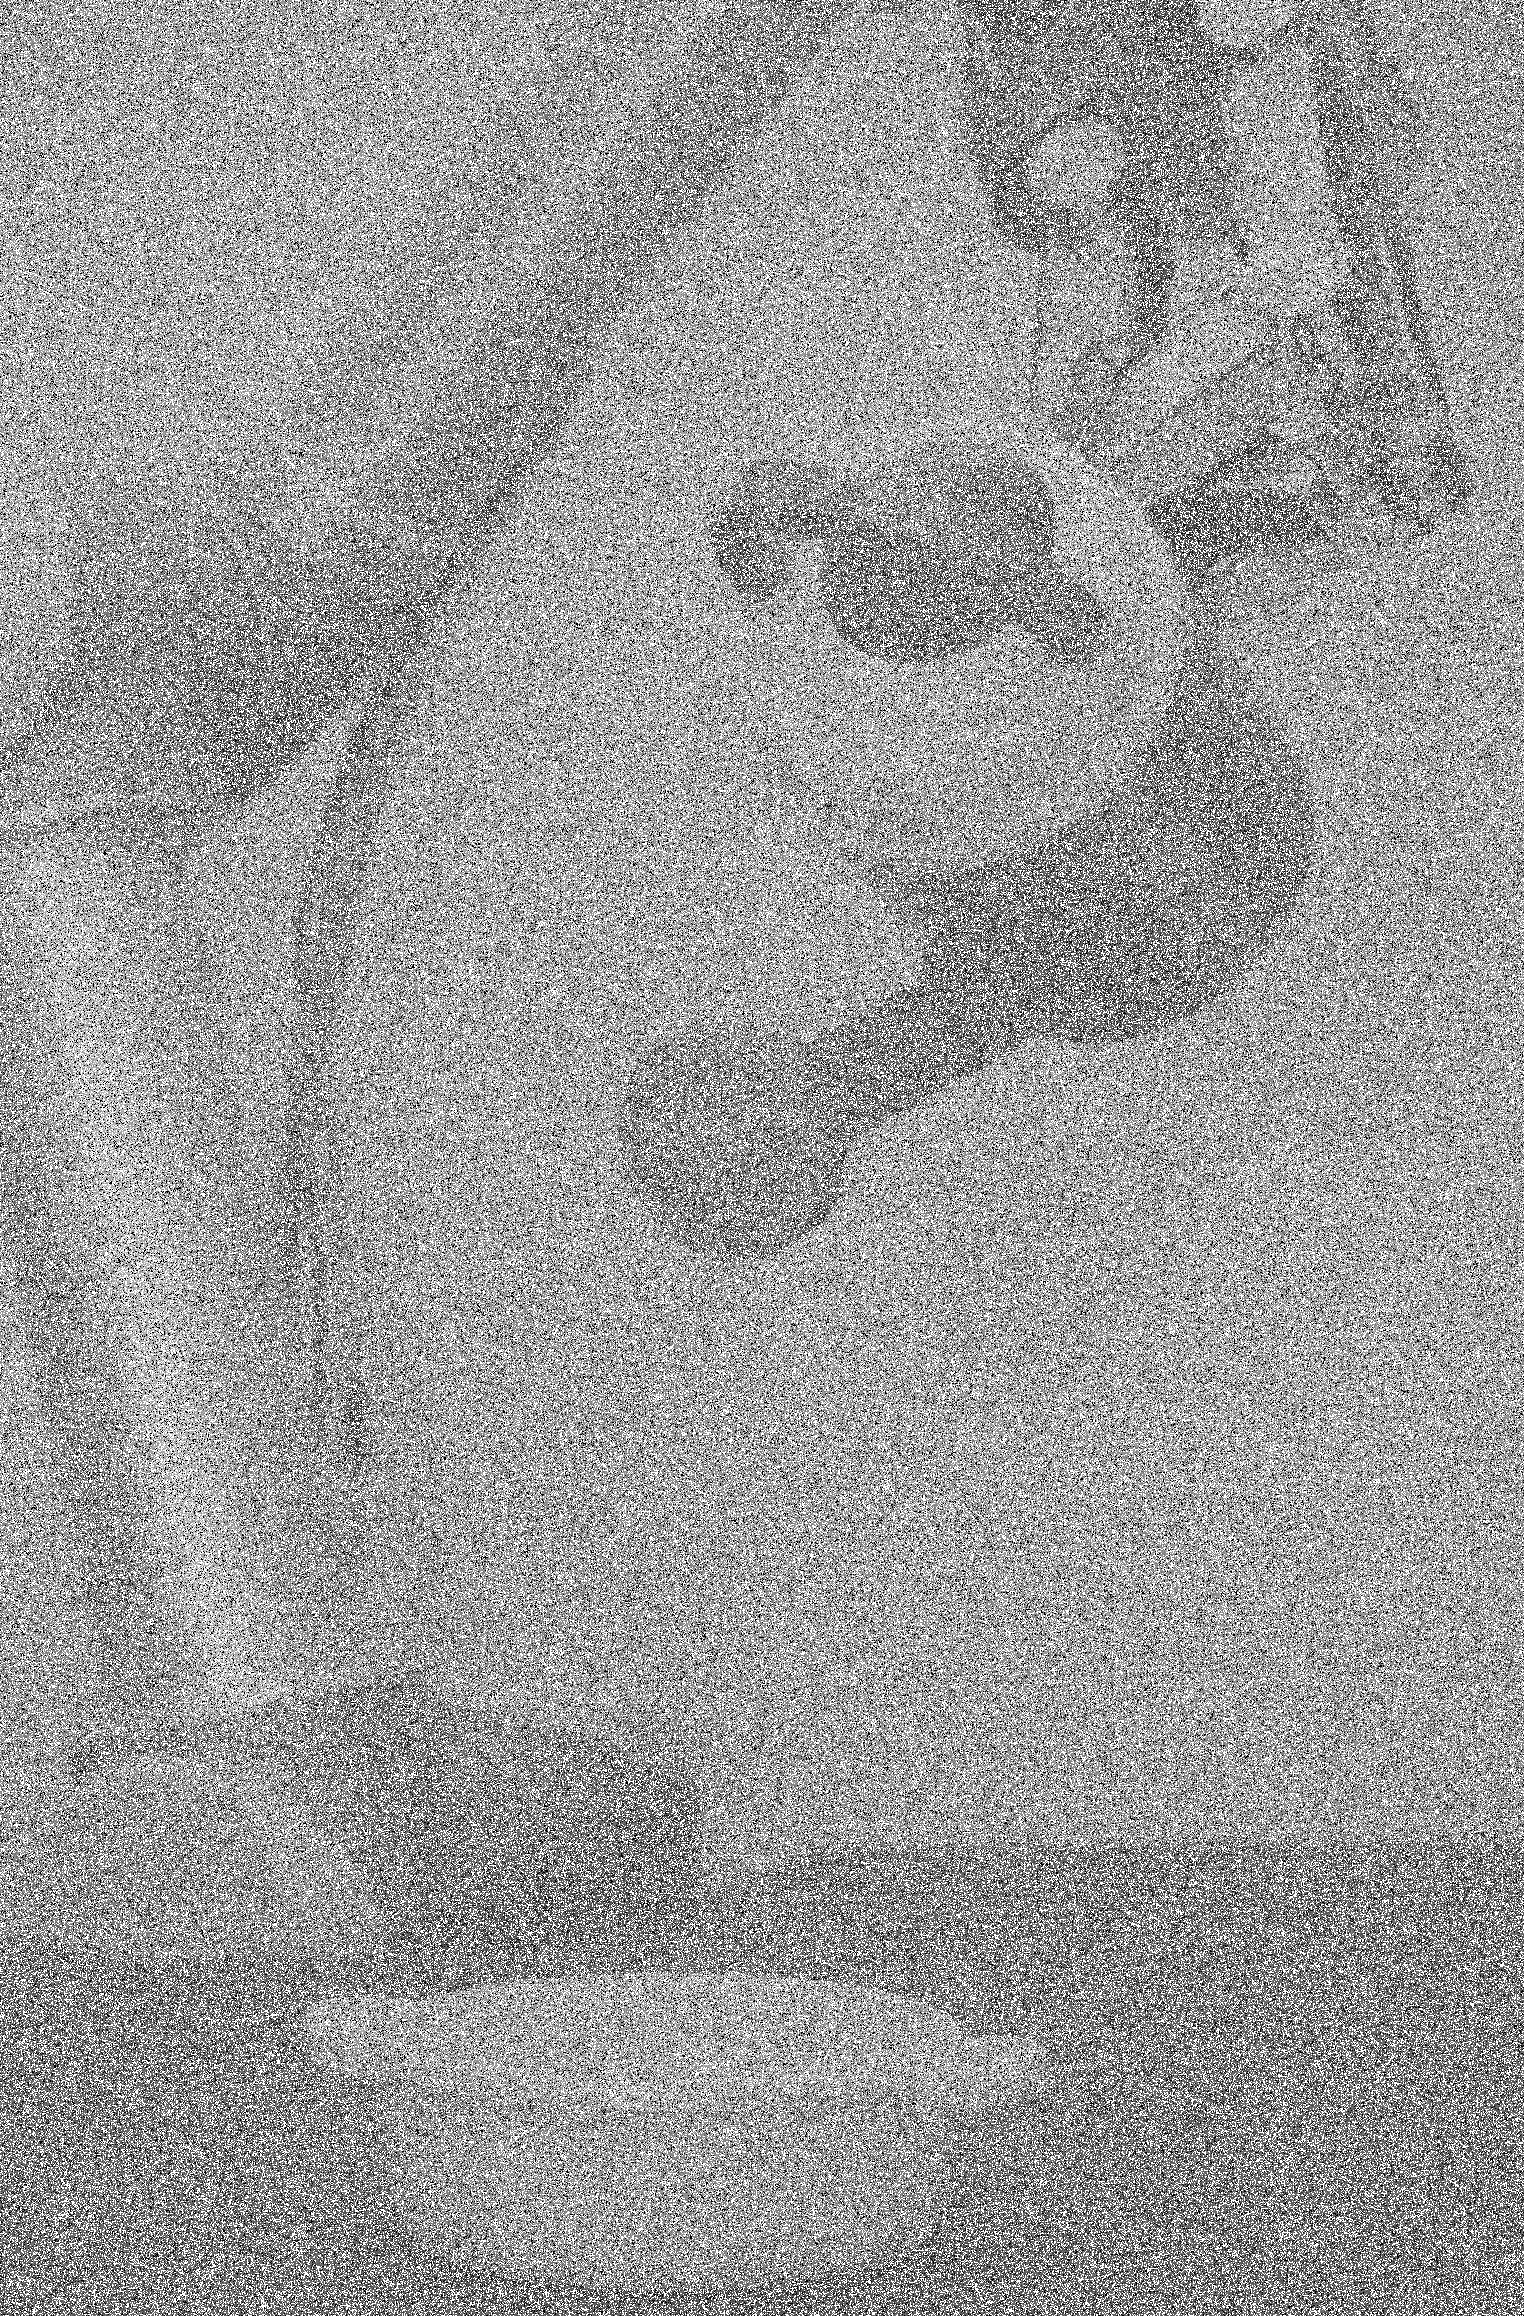
\includegraphics[width=\textwidth]{img2/src.png}
        \caption{The original image}
        \label{fig:img2_src}
    \end{subfigure}
    \begin{subfigure}[b]{0.446\textwidth}
        
\includegraphics[width=\textwidth]{img2/hist.png}
        \caption{Histogram of the original image}
        \label{fig:img2_hist}
    \end{subfigure}
    \caption{Analysis of image 2}\label{fig:img2}
\end{figure}

Approximately  there are three times more salt noise compared to the pepper noise. The values in the middle of the histogram is what is left of the original image, and in order to restore as much as possible, and median filter is applied on the image. \todo{How do we know.. det kunne også være en form for noise, vi ved kun med sikkerhed at pepper of salt er tydeligt. hvilket kan ses og bekræftes via hist. }The median filter is chosen because it is very effective against salt-and-pepper noise in the images, and the OpenCV function
\begin{center}
\lstinline|void medianBlur(InputArray src, OutputArray dst, int ksize)|\footnote{\url{http://docs.opencv.org/2.4/modules/imgproc/doc/filtering.html\#void medianBlur(InputArray src, OutputArray dst, int ksize)}}
\end{center}
is used for applying this filter to the image. The median filter help blurring the image, and depending on the size of \lstinline|ksize|, the more blurred will the image become.\\[0.2cm]
The \lstinline|ksize| is the size of the kernel filter applied to each pixel in the image, and therefore must the value of \lstinline|ksize| be odd and greater than 1, so in order to test if the noise is removed, a kernel of \lstinline|3| is applied on the image 2 and checked if all the noise is removed. If not all the noise is removed, the kernel size is increased with two, and checked again, and so on.  

\begin{figure}[H]
    \centering
    \begin{subfigure}[b]{0.24\textwidth}
        \includegraphics[width=\textwidth]{img2/median3.png}\\[0.1cm]
        
\includegraphics[width=\textwidth]{img2/kernel3.png}
        \caption{\lstinline|ksize = 3|}
        \label{fig:img2_kernel3}
    \end{subfigure}
    \begin{subfigure}[b]{0.24\textwidth}
        \includegraphics[width=\textwidth]{img2/median5.png}\\[0.1cm]
        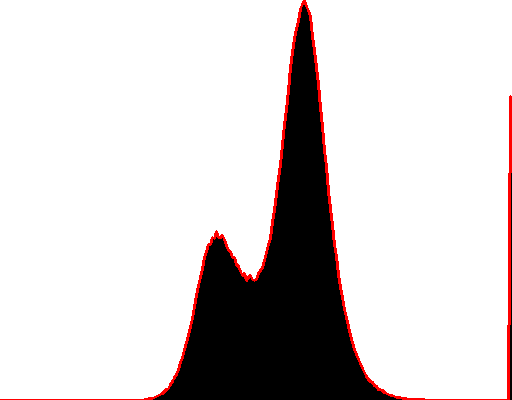
\includegraphics[width=\textwidth]{img2/kernel5.png}
        \caption{\lstinline|ksize = 5|}
        \label{fig:img2_kernel5}
    \end{subfigure}
    \begin{subfigure}[b]{0.24\textwidth}
        \includegraphics[width=\textwidth]{img2/median7.png}\\[0.1cm]
        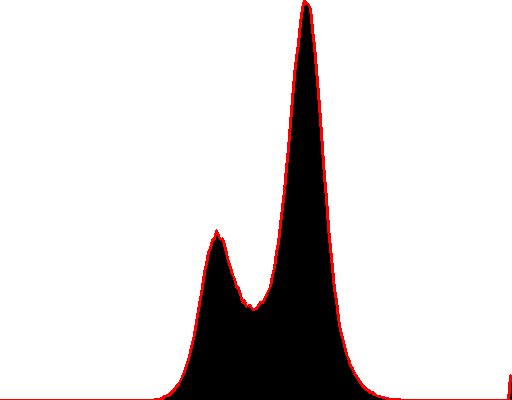
\includegraphics[width=\textwidth]{img2/kernel7.png}
        \caption{\lstinline|ksize = 7|}
        \label{fig:img2_kernel7}
    \end{subfigure}
    \begin{subfigure}[b]{0.24\textwidth}
        \includegraphics[width=\textwidth]{img2/median9.png}\\[0.1cm]
        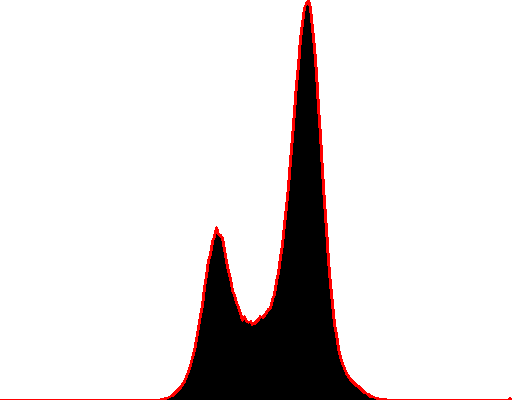
\includegraphics[width=\textwidth]{img2/kernel9.png}
        \caption{\lstinline|ksize = 9|}
        \label{fig:img2_kernel9}
    \end{subfigure}
    \caption{Analysis of image 2}\label{fig:img2}
\end{figure}
Figure \ref{fig:img2_kernel3}, \ref{fig:img2_kernel5}, \ref{fig:img2_kernel7} and \ref{fig:img2_kernel9} shows the process of finding the right \lstinline|ksize|, but all four kernel sizes still does not remove all the noise, especially the salt noise. All the salt--and--pepper noise is removed with a \lstinline|ksize=11|, but the disadvantage of this approach is that the details in the image are reduced. For restoring as much as possible of the these details, a histogram equalization is applied on the noise reduced image. Histogram equalization restores the details by improves the contrast in the image by stretching out the intensity range of the image. On the left and right side of image \ref{fig:img2_kernel11}'s histogram are there underpopulated intensities, which is why an histogram equalization is an optimal choice. The result is shown on figure \ref{fig:img2_histEq}.
\begin{figure}[H]
    \centering
    \begin{subfigure}[b]{0.3\textwidth}
        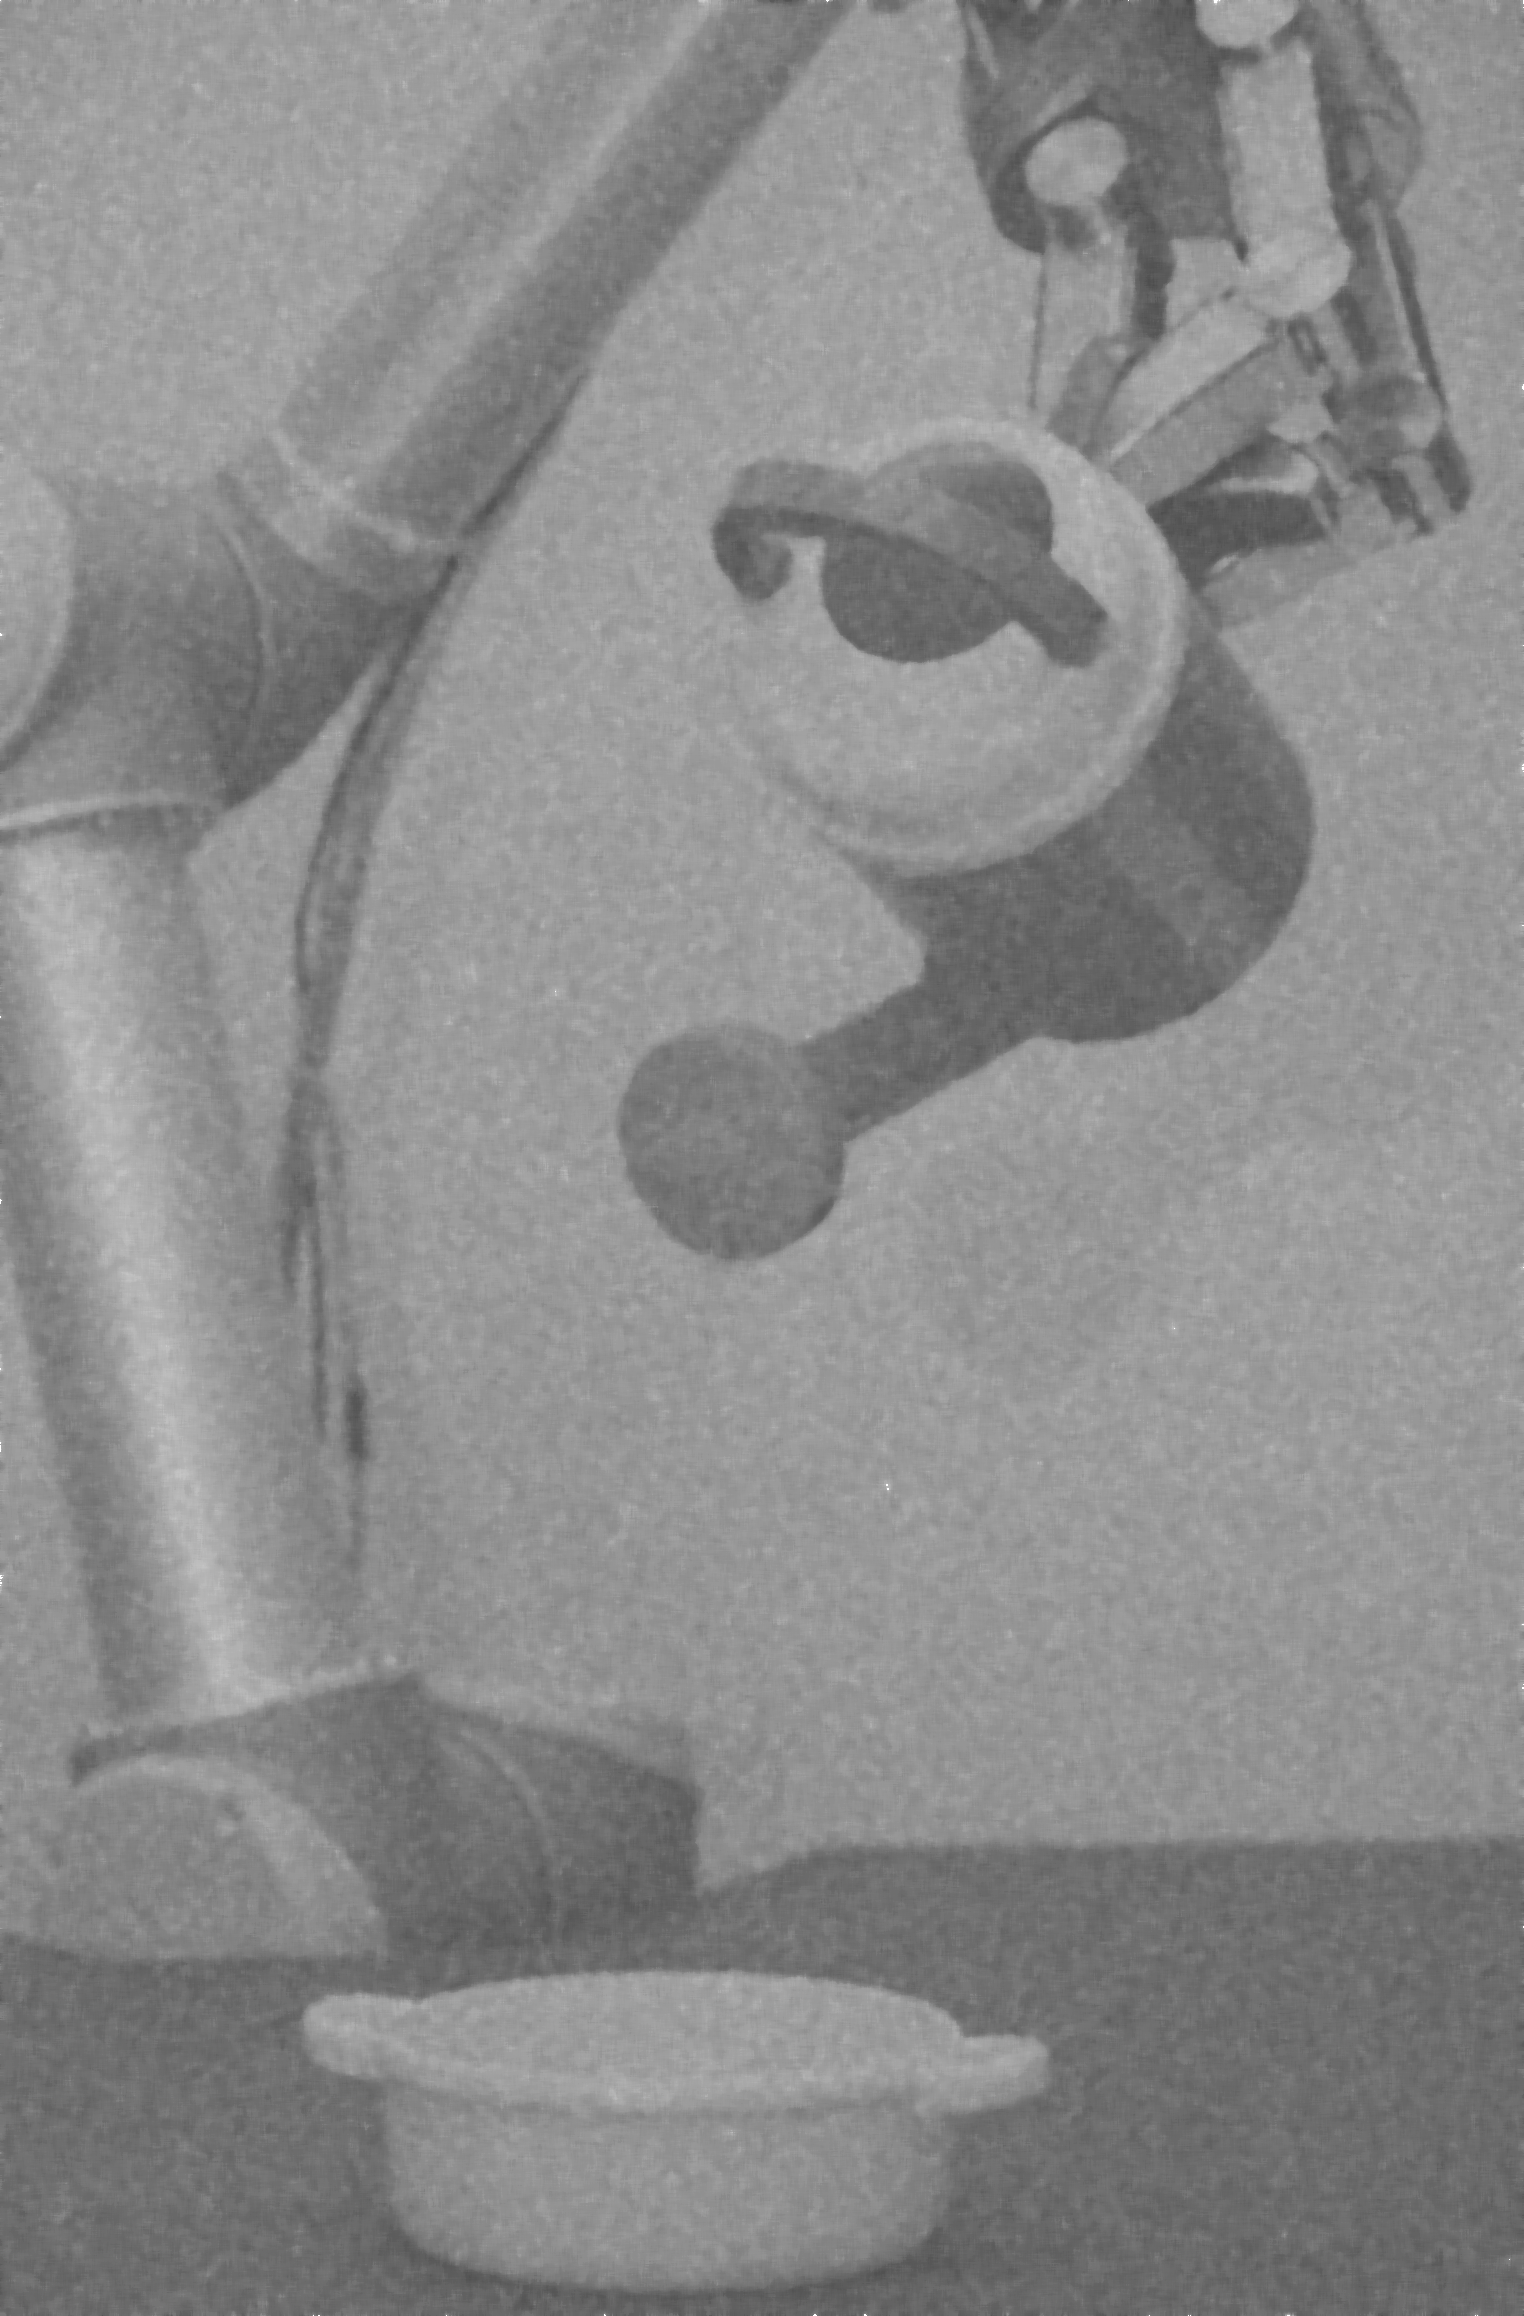
\includegraphics[width=\textwidth]{img2/median.png}\\[0.1cm]
        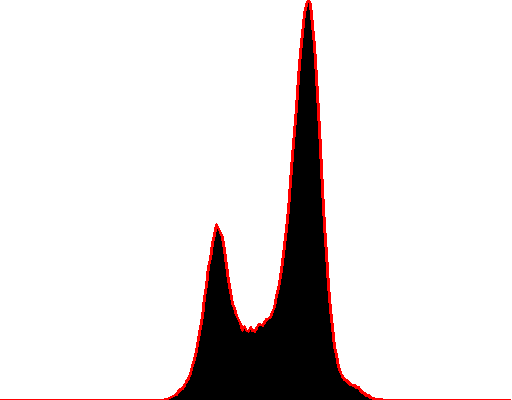
\includegraphics[width=\textwidth]{img2/histn.png}
        \caption{\lstinline|ksize = 11|}
        \label{fig:img2_kernel11}
    \end{subfigure}
    \begin{subfigure}[b]{0.3\textwidth}
        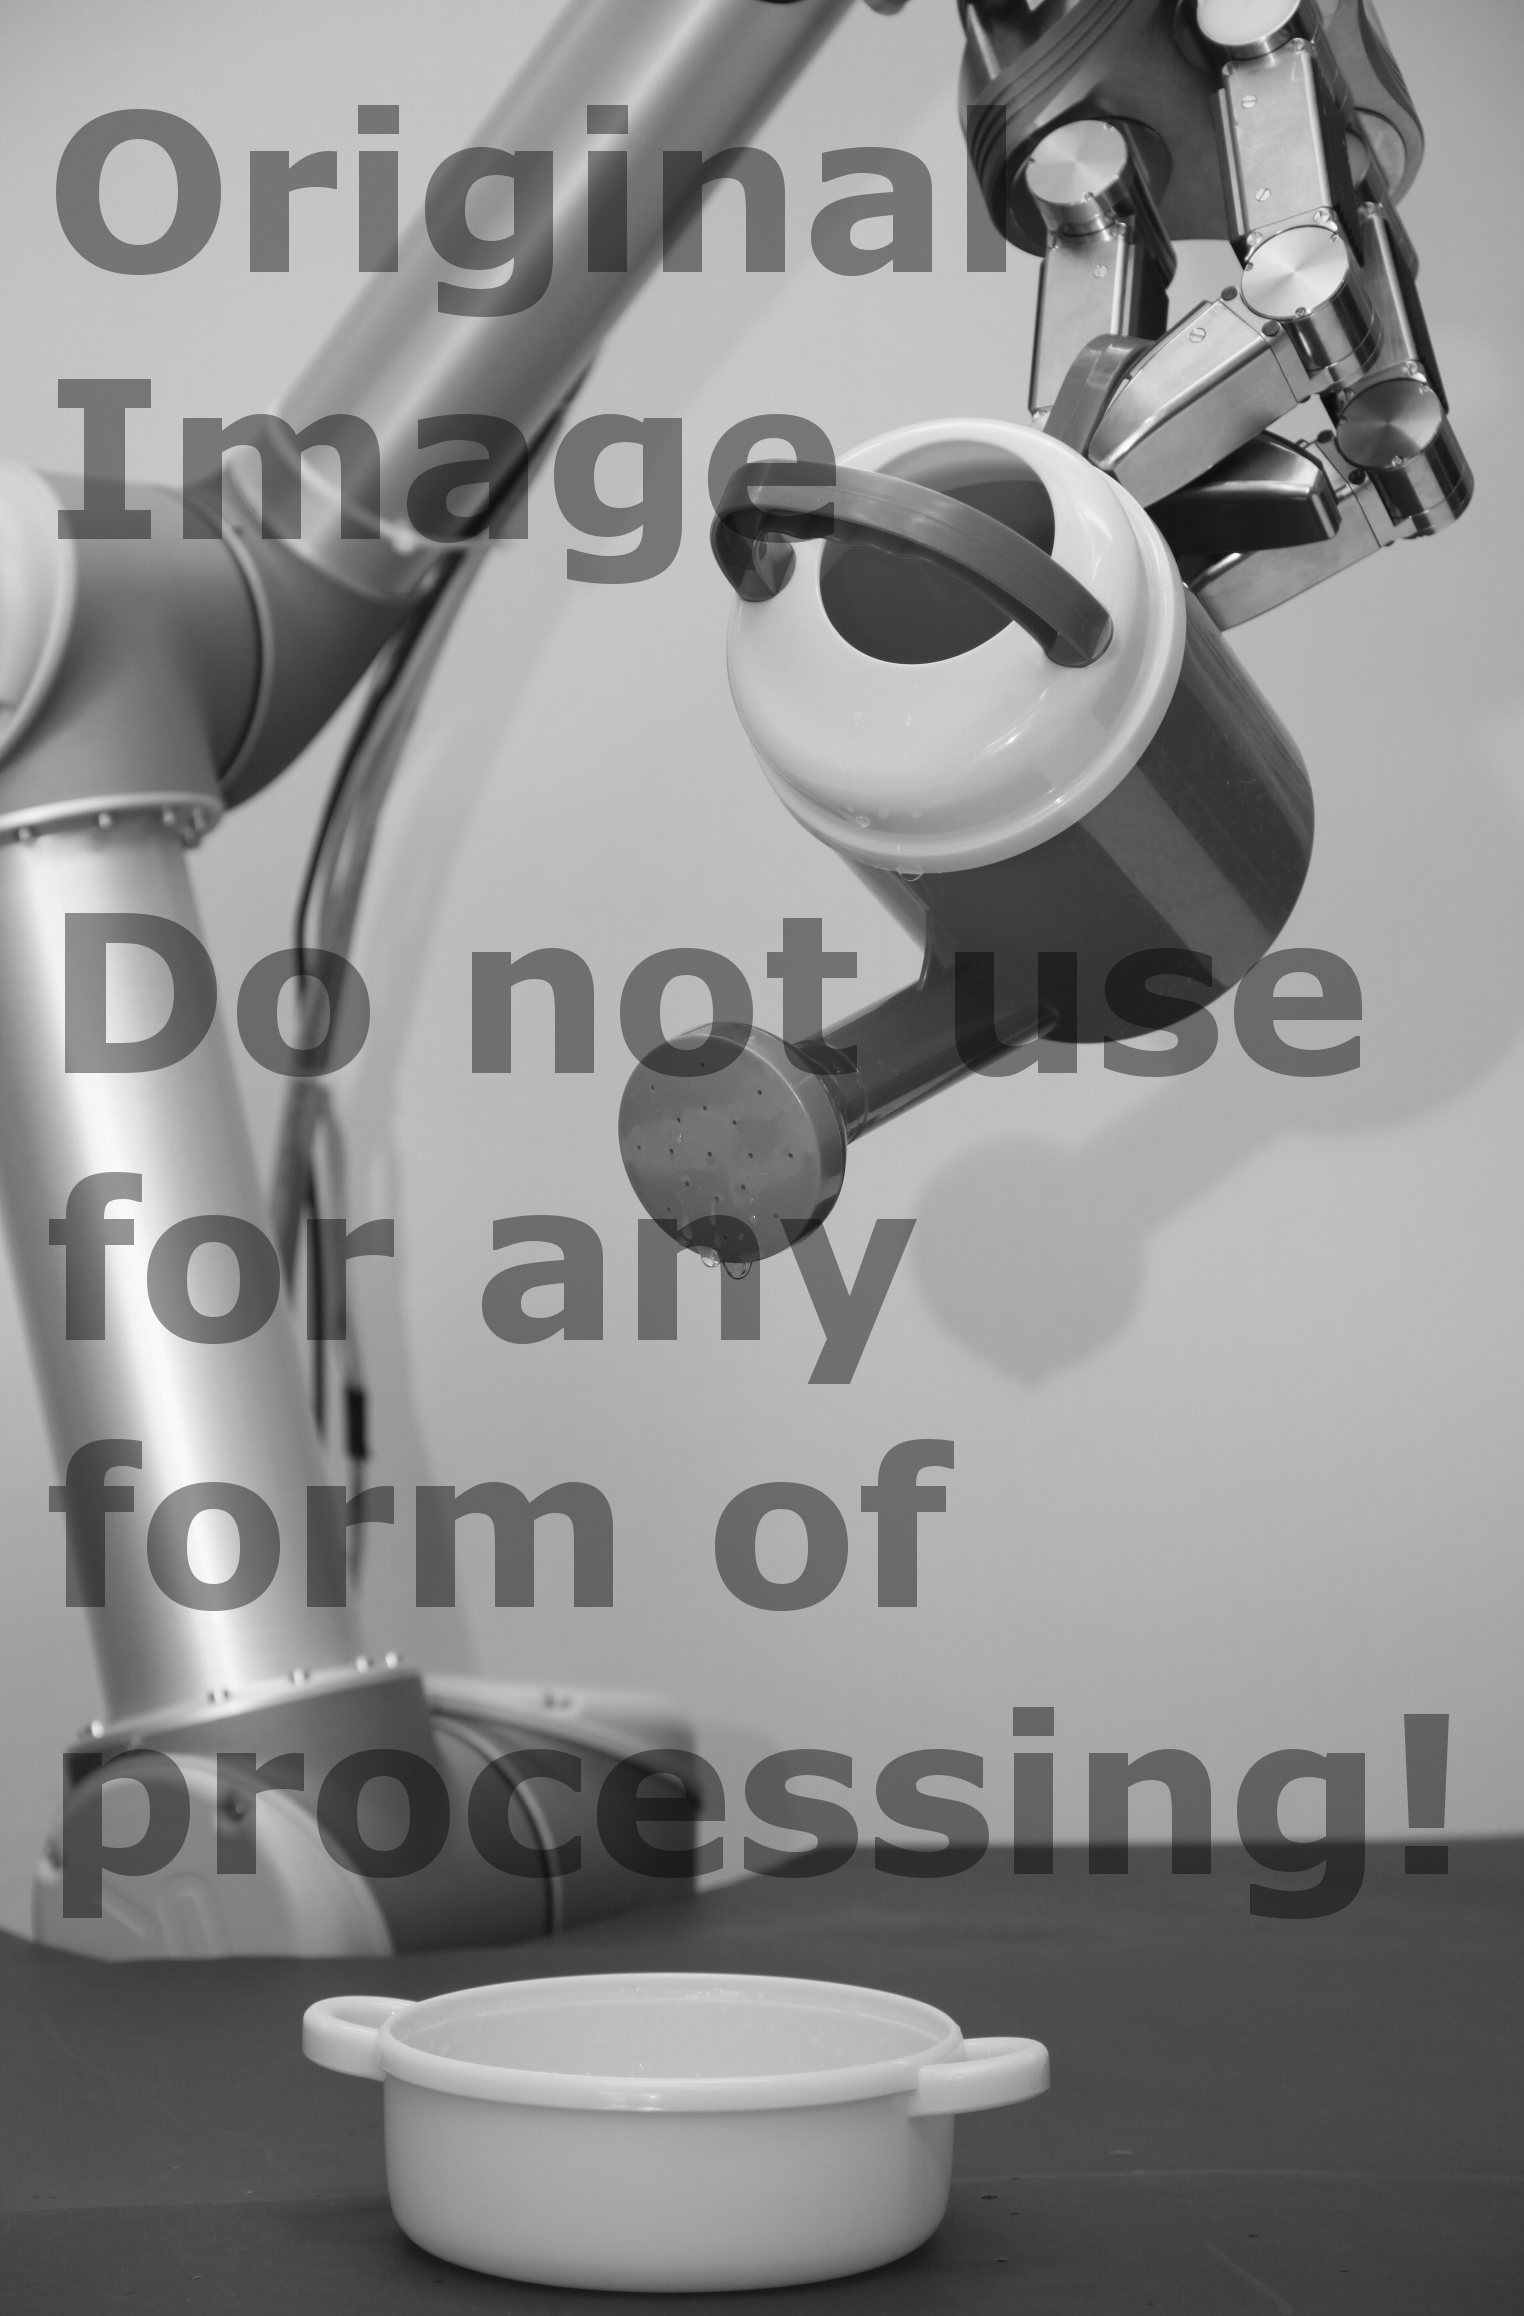
\includegraphics[width=\textwidth]{org.png}\\[0.1cm]
        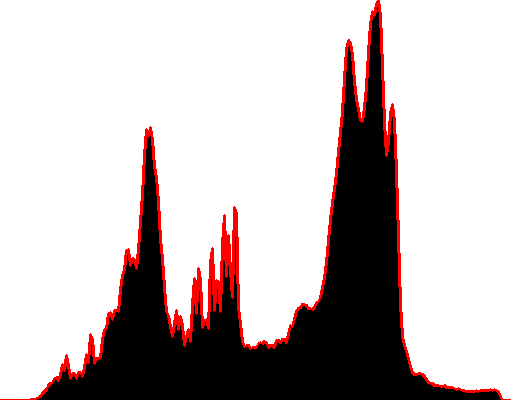
\includegraphics[width=\textwidth]{histOrg.png}
        \caption{Equalized}
        \label{fig:img2_org}
    \end{subfigure}
    \begin{subfigure}[b]{0.3\textwidth}
        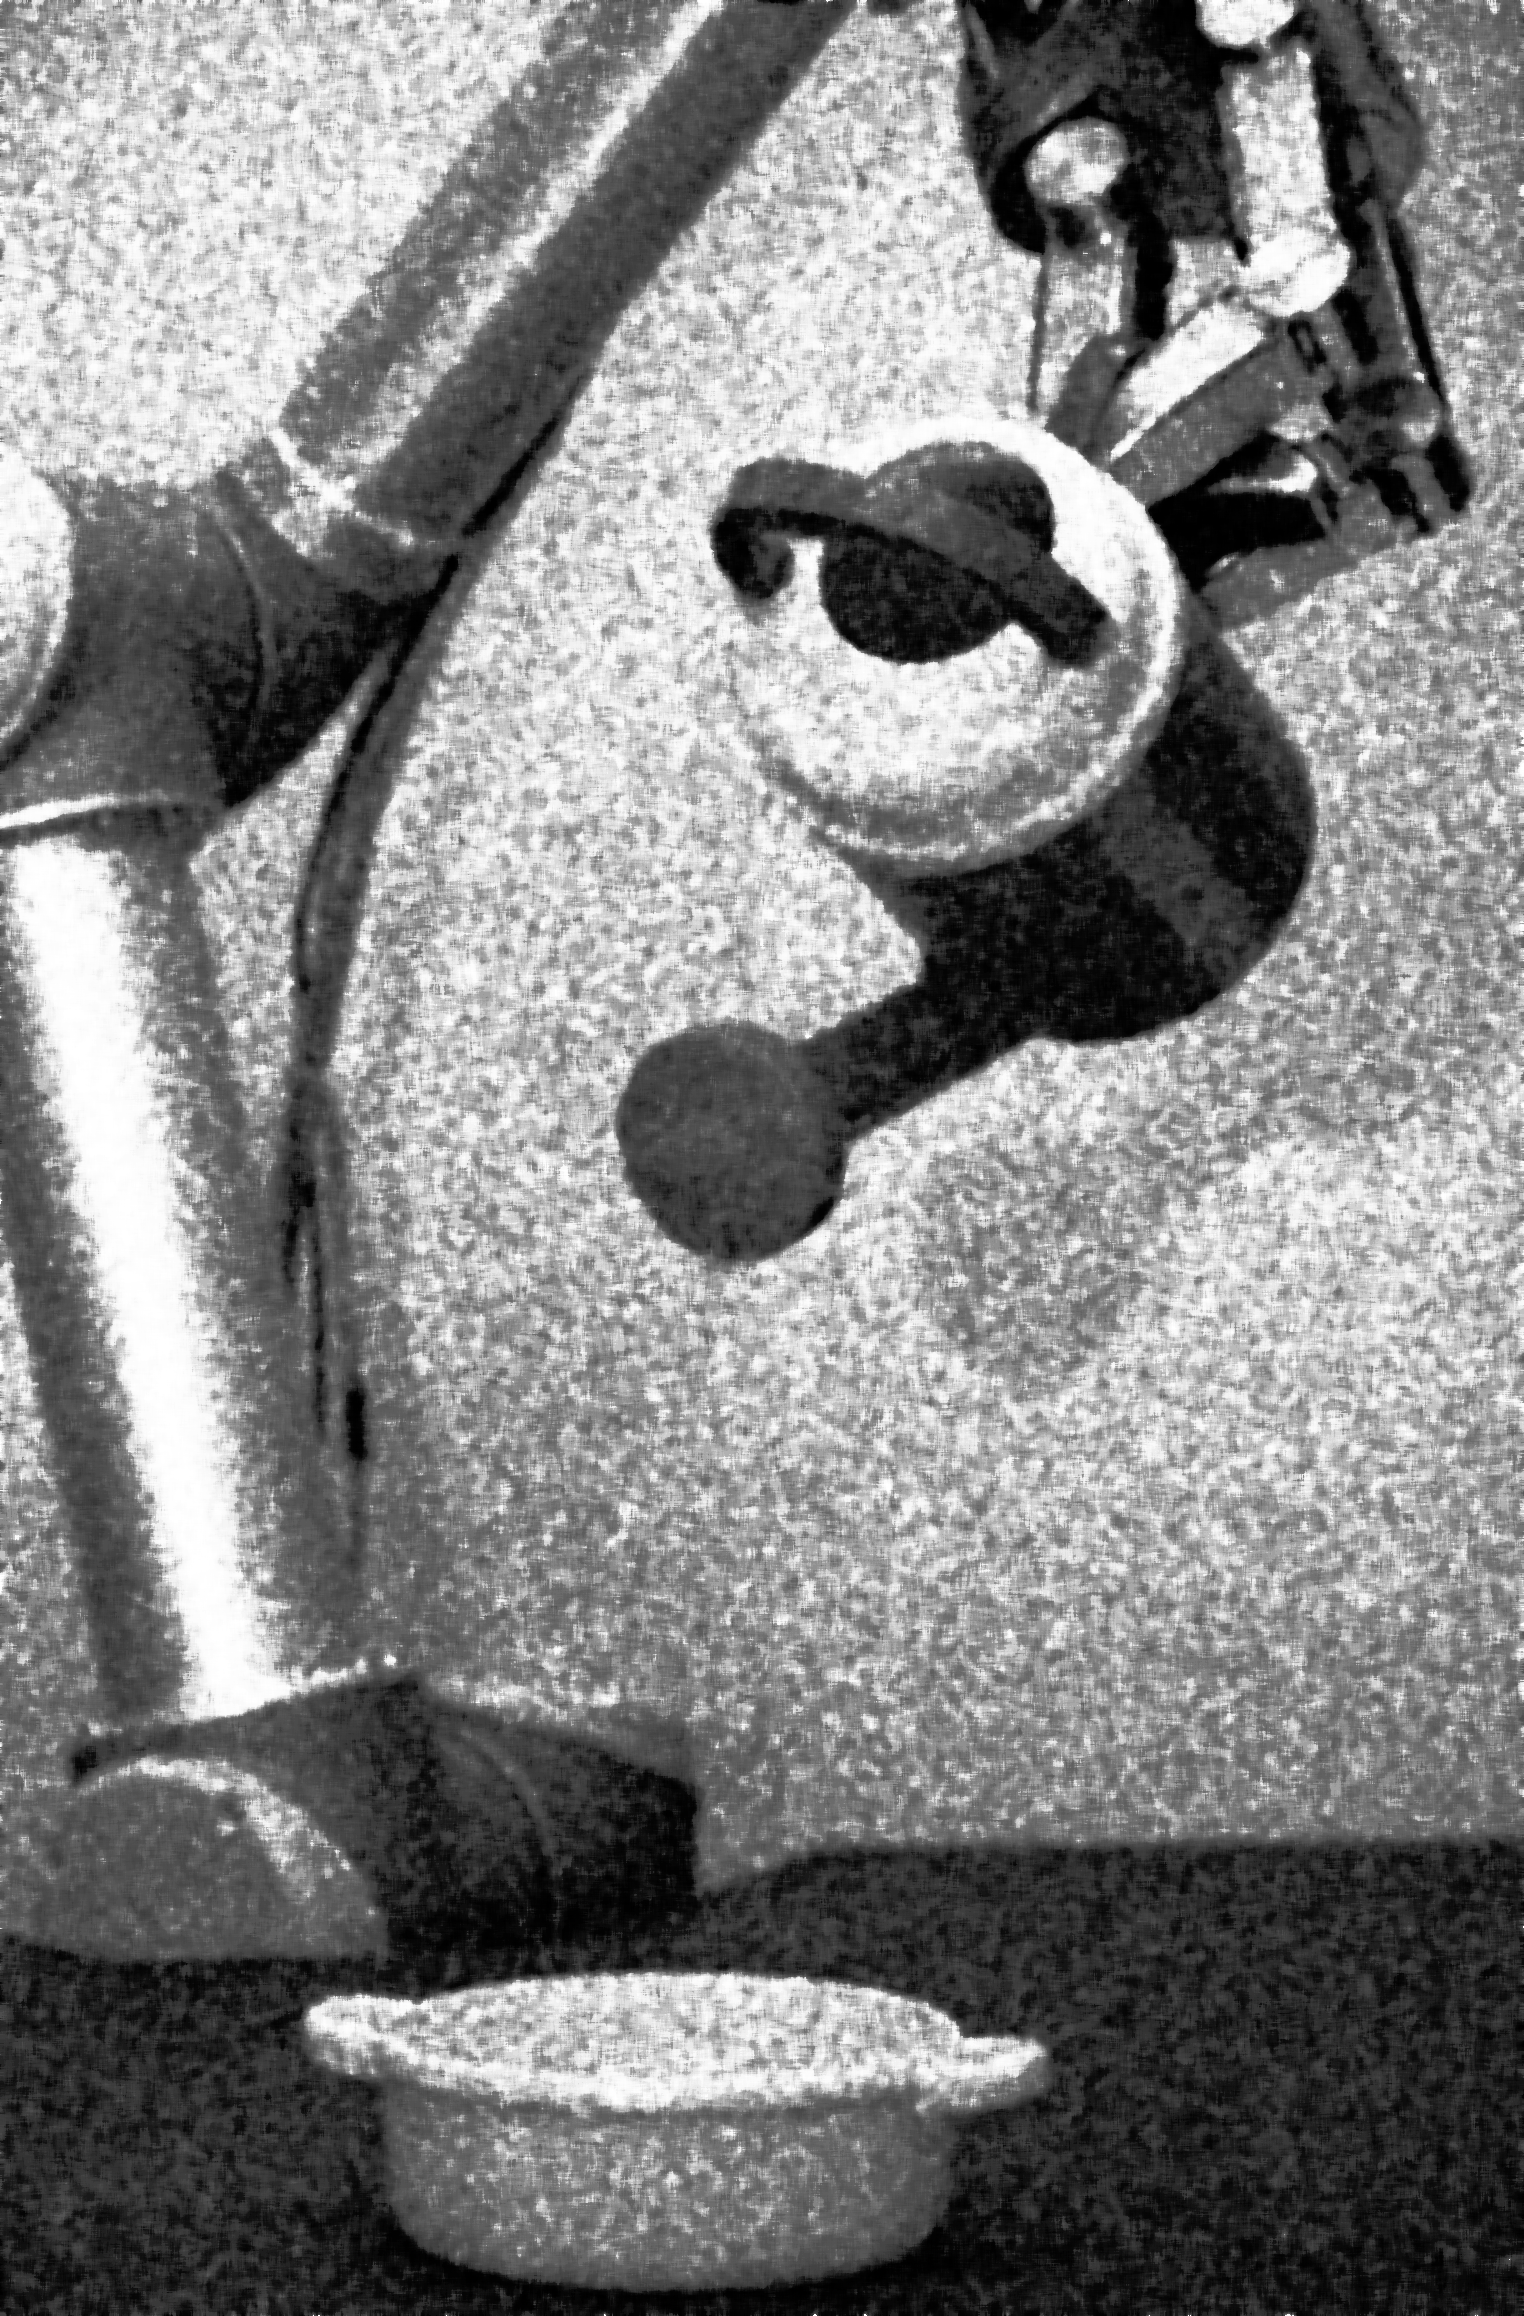
\includegraphics[width=\textwidth]{img2/eqlMedian.png}\\[0.1cm]
        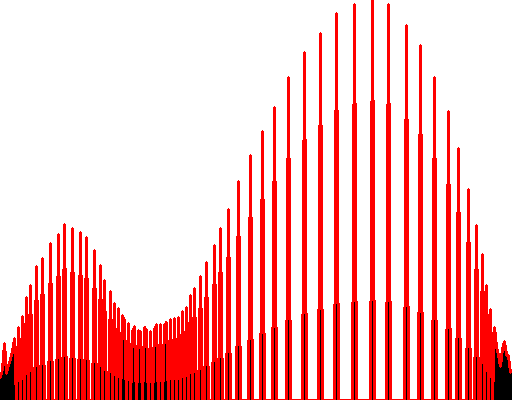
\includegraphics[width=\textwidth]{img2/histE.png}
        \caption{Equalized}
        \label{fig:img2_histEq}
    \end{subfigure}
    \caption{Analysis of image 2}\label{fig:img2}
\end{figure}
\todo[inline]{Which one is best? -- conclusion needed.. Try contrast streching.. fremfor equalization}

\section{Image 3}
Figure \ref{fig:img3} shows the original image with some kind of white noise in it, and by analysing the image histogram (image \ref{fig:img3_hist}) can two kind of noise fit this: Gaussian noise (figure \ref{fig:noise_gaussian}) and uniform noise (figure \ref{fig:noise_uniform}).

\begin{figure}[H]
    \centering
    \begin{subfigure}[b]{0.25\textwidth}
        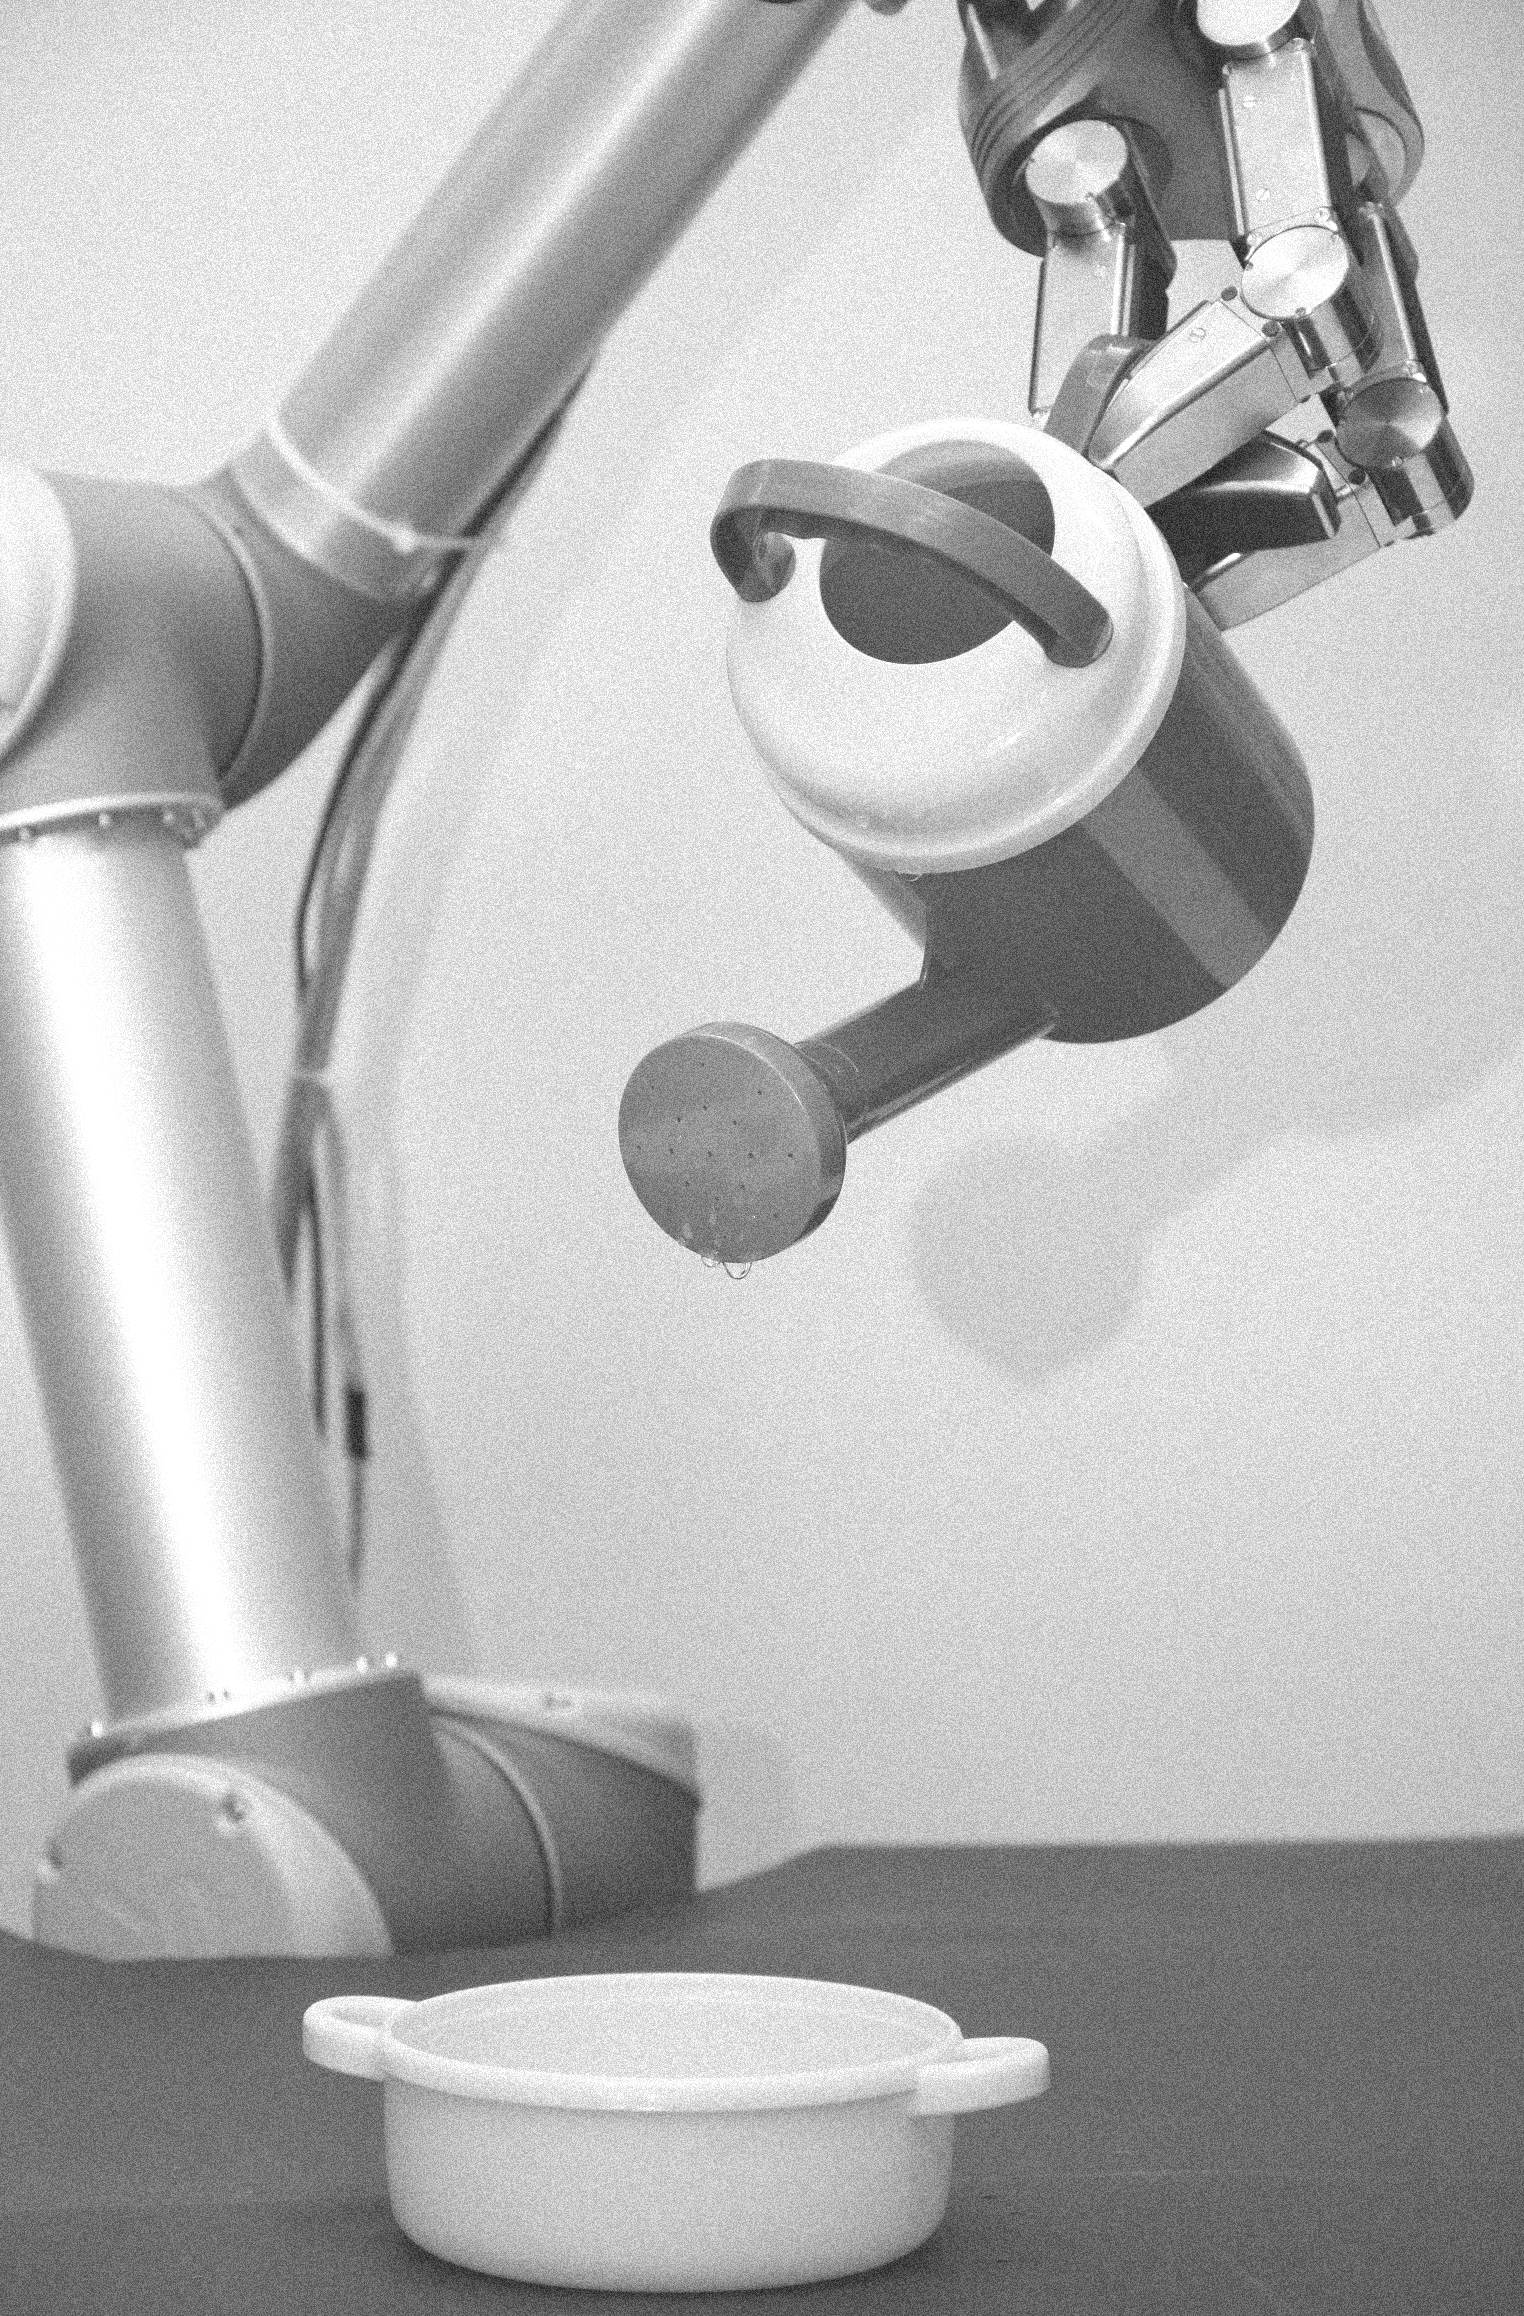
\includegraphics[width=\textwidth]{img3/src.png}
        \caption{The original image}
        \label{fig:img3_src}
    \end{subfigure}
    \begin{subfigure}[b]{0.485\textwidth}
        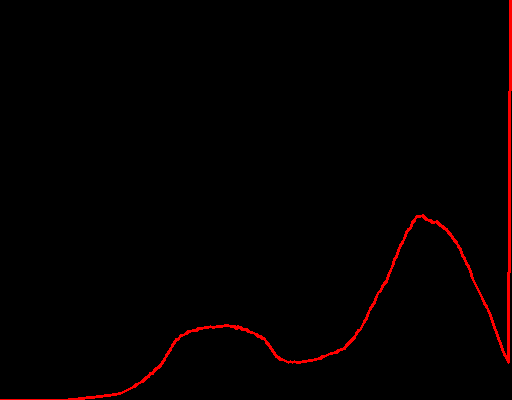
\includegraphics[width=\textwidth]{img3/hist_org_img3.png}
        \caption{Histogram of the original image}
        \label{fig:img3_hist}
    \end{subfigure}
    \caption{Analysis of image 3}
    \label{fig:img3}
\end{figure}
In order to determine which kind of noise it is, an uniform surface of the image is analysed, as shown on figure \todo{Vi har vel tjekket alle  histogram for alle i uniforme overflader.. Det vel en selvfølge, så vi burde nok skrive det et sted..} \ref{fig:rect_org_img3}. By comparing the histogram of the uniform surface in figure \ref{fig:rect_org_img3} with the two noise examples histograms in figure \ref{fig:noise_examples_img3}, it can be determined that as the noise in image \ref{fig:img3_src} mostly resembles uniform noise,   it is also present in the image . 

\begin{figure}[H]
    \centering
    \begin{subfigure}[b]{0.22\textwidth}
        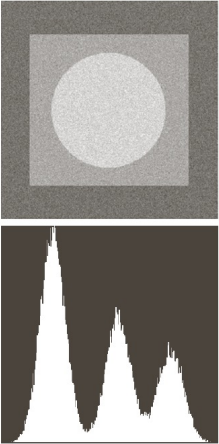
\includegraphics[width=\textwidth]{img3/noise_g.png}
        \caption{Gaussian noise}
        \label{fig:noise_gaussian}
    \end{subfigure}
    \begin{subfigure}[b]{0.2175\textwidth}
        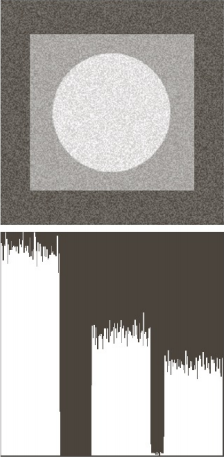
\includegraphics[width=\textwidth]{img3/noise_u.png}
        \caption{Uniform noise}
        \label{fig:noise_uniform}
    \end{subfigure}
    \caption{Examples of different noise models}
    \label{fig:noise_examples_img3}
\end{figure}

\begin{figure}[H]
    \centering
    \begin{subfigure}[b]{0.24\textwidth}
        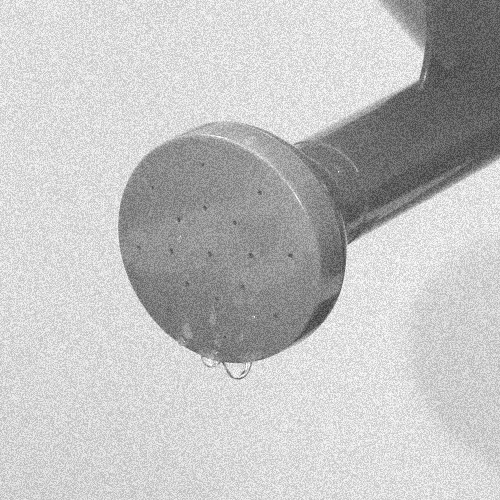
\includegraphics[width=\textwidth]{img3/rect_org_img3.png}
        \begin{center}
        	\textbf{Uniform surfaces}
        \end{center}
        
\includegraphics[width=\textwidth]{img3/rect_src_img3.png}\\[0.1cm]
        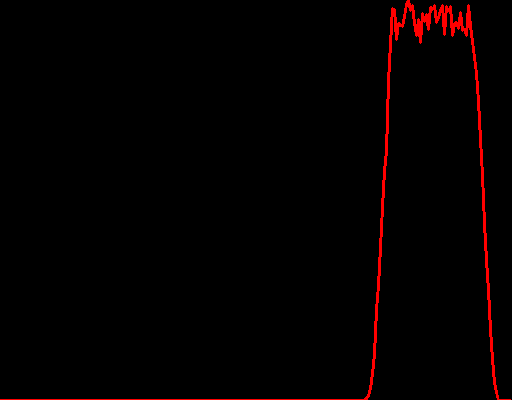
\includegraphics[width=\textwidth]{img3/hist_rect_src_img3.png}
        \caption{The original image}
        \label{fig:rect_org_img3}
    \end{subfigure}
    \begin{subfigure}[b]{0.24\textwidth}
        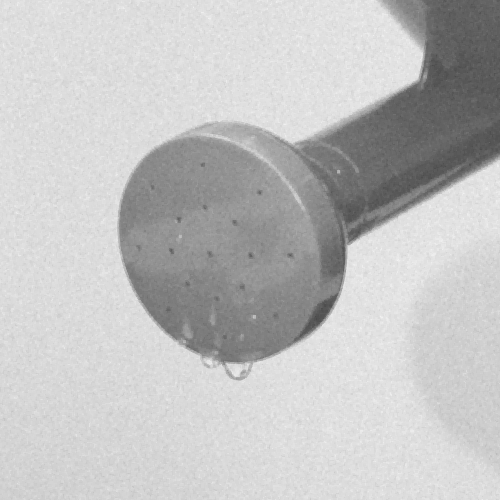
\includegraphics[width=\textwidth]{img3/rect_3_midpoint_3_final_img3_add.png}
        \begin{center}
        	\text{ }
        \end{center}
        
\includegraphics[width=\textwidth]{img3/rect_3_midpoint_3_final_img3.png}\\[0.1cm]
        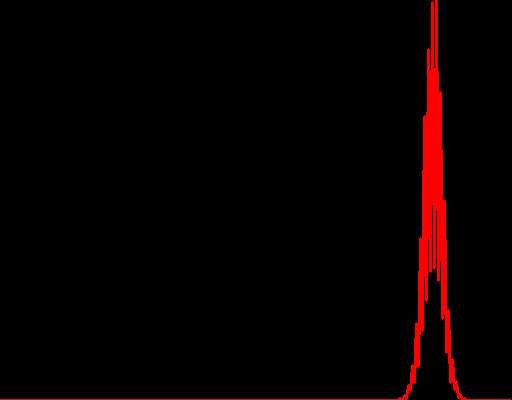
\includegraphics[width=\textwidth]{img3/hist_rect_3_midpoint_3_final_img3.png}
        \caption{Kernel 3}
        \label{fig:img3_kernel_3}
    \end{subfigure}
    \begin{subfigure}[b]{0.24\textwidth}
        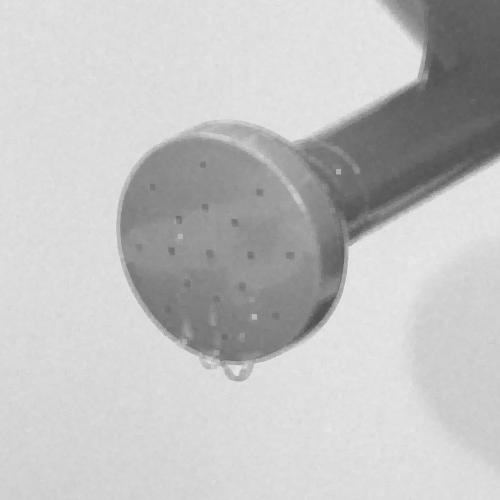
\includegraphics[width=\textwidth]{img3/rect_5_midpoint_5_final_img3_add.png}
        \begin{center}
        	\text{ }
        \end{center}
        
\includegraphics[width=\textwidth]{img3/rect_5_midpoint_5_final_img3.png}\\[0.1cm]
        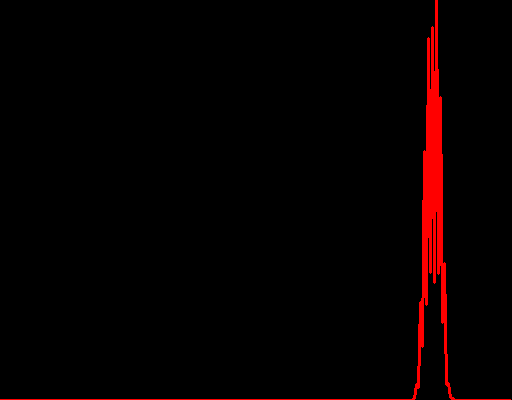
\includegraphics[width=\textwidth]{img3/hist_rect_5_midpoint_5_final_img3.png}
        \caption{Kernel 5}
        \label{fig:img3_kernel_5}
    \end{subfigure}
    \begin{subfigure}[b]{0.24\textwidth}
        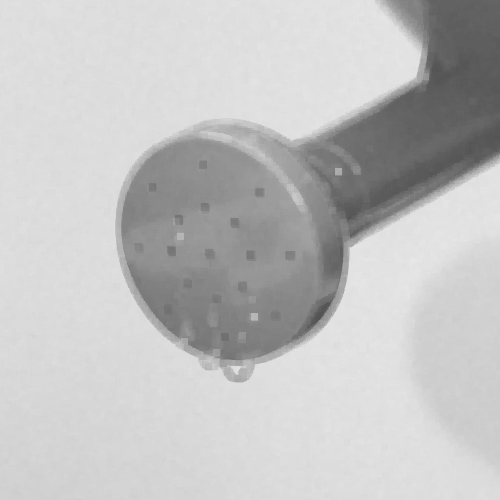
\includegraphics[width=\textwidth]{img3/rect_7_midpoint_7_final_img3_add.png}
        \begin{center}
        	\text{ }
        \end{center}
        
\includegraphics[width=\textwidth]{img3/rect_7_midpoint_7_final_img3.png}\\[0.1cm]
        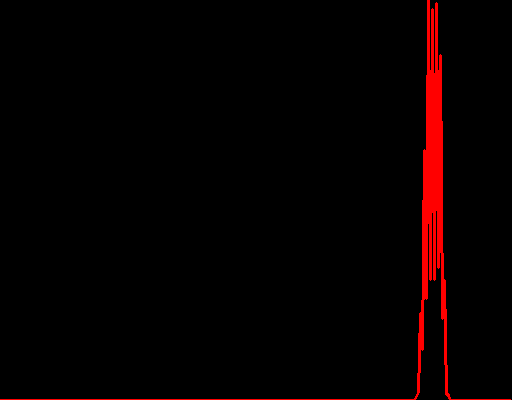
\includegraphics[width=\textwidth]{img3/hist_rect_7_midpoint_7_final_img3.png}
        \caption{Kernel 7}
        \label{fig:img3_kernel_7}
    \end{subfigure}
    \caption{Analysis of image 3}
    \label{fig:img3_kernel}
\end{figure}

In order to reduce the uniform noise in the image, a midpoint filter is applied to the image, as it is effective against Gaussian noise and uniform noise \todo{ref}. The method works be replacing the pixel with the average value (i.e. the midpoint) of the minimum pixel and maximum pixel within an kernel.  The kernel size must be odd and greater than 1, and the greater the kernel size is, the greater are the effects , but the image becomes more pixelated especially at the edges.  \\[0.2cm]
Figure \ref{fig:img3_kernel_3}, \ref{fig:img3_kernel_5} and \ref{fig:img3_kernel_7} shows the result of three different kernel sizes; 3, 5 and 7. By comparing the same uniform surface of each of the images, can it be seen that a kernel 3 does not remove all the noise, but kernel 5 and 7 does. By comparing the sharpness of the edges with a kernel 5 and a kernel 7, the kernel 7's edges is too pixelated compared to the edges in kernel 5, and that is why in this project a midpoint filter with a kernel 5 is chosen to be applied in order to remove the uniform noise in image \ref{fig:img3_src}.\\[0.2cm]
Figure \ref{fig:img3_kernel_5_final} shows the full image after applying the midpoint filter with a kernel size of 5, and compared to the original image (figure \ref{fig:img3_org_final}) it can be seen that there is a difference in the brightness. Figure \ref{fig:img3_kernel_5_final} is brighter than the original image, and therefore is the OpenCV function used
\begin{center}
\lstinline|void Mat::convertTo(OutputArray m, int rtype, double alpha=1, double beta=0 )|\footnote{\url{http://docs.opencv.org/2.4/modules/core/doc/basic_structures.html\#mat-convertto}}
\end{center}
and by changing the \lstinline|alpha| is it possible equalizing the brightness between the source image and the original image as much as possible. An \lstinline|alpha| lower than 1 will darken the image, and an \lstinline|alpha| higher than 1 will brighten the image. Figure \ref{fig:img3_test_brightness} shows the result of some different values of \lstinline|aplha|, where the first row is an \lstinline|alpha| value below 1 and the second row is an \lstinline|alpha| above 1. Finding the right \lstinline|alpha| is done by testing with different values below 1, similar to the first row in figure \ref{fig:img3_test_brightness}, with an step of 0.05, and the best fit was found to be an \lstinline|alphe=0.85|, so 
\begin{center}
\lstinline|scr.convertTo(dst, -1, 0.85, 0)|
\end{center}
and the result of this is shown on figure \ref{fig:img3_contrast}. After this equalization  of the brightness can it also be seen that the full histogram of figure \ref{fig:img3_contrast} look a lot more similar to figure \ref{fig:img3_org_final}'s full histogram, compared to figure \ref{fig:img3_kernel_5_final}'s histogram.

\begin{figure}[H]
    \centering
    \begin{subfigure}[b]{0.1\textwidth}
        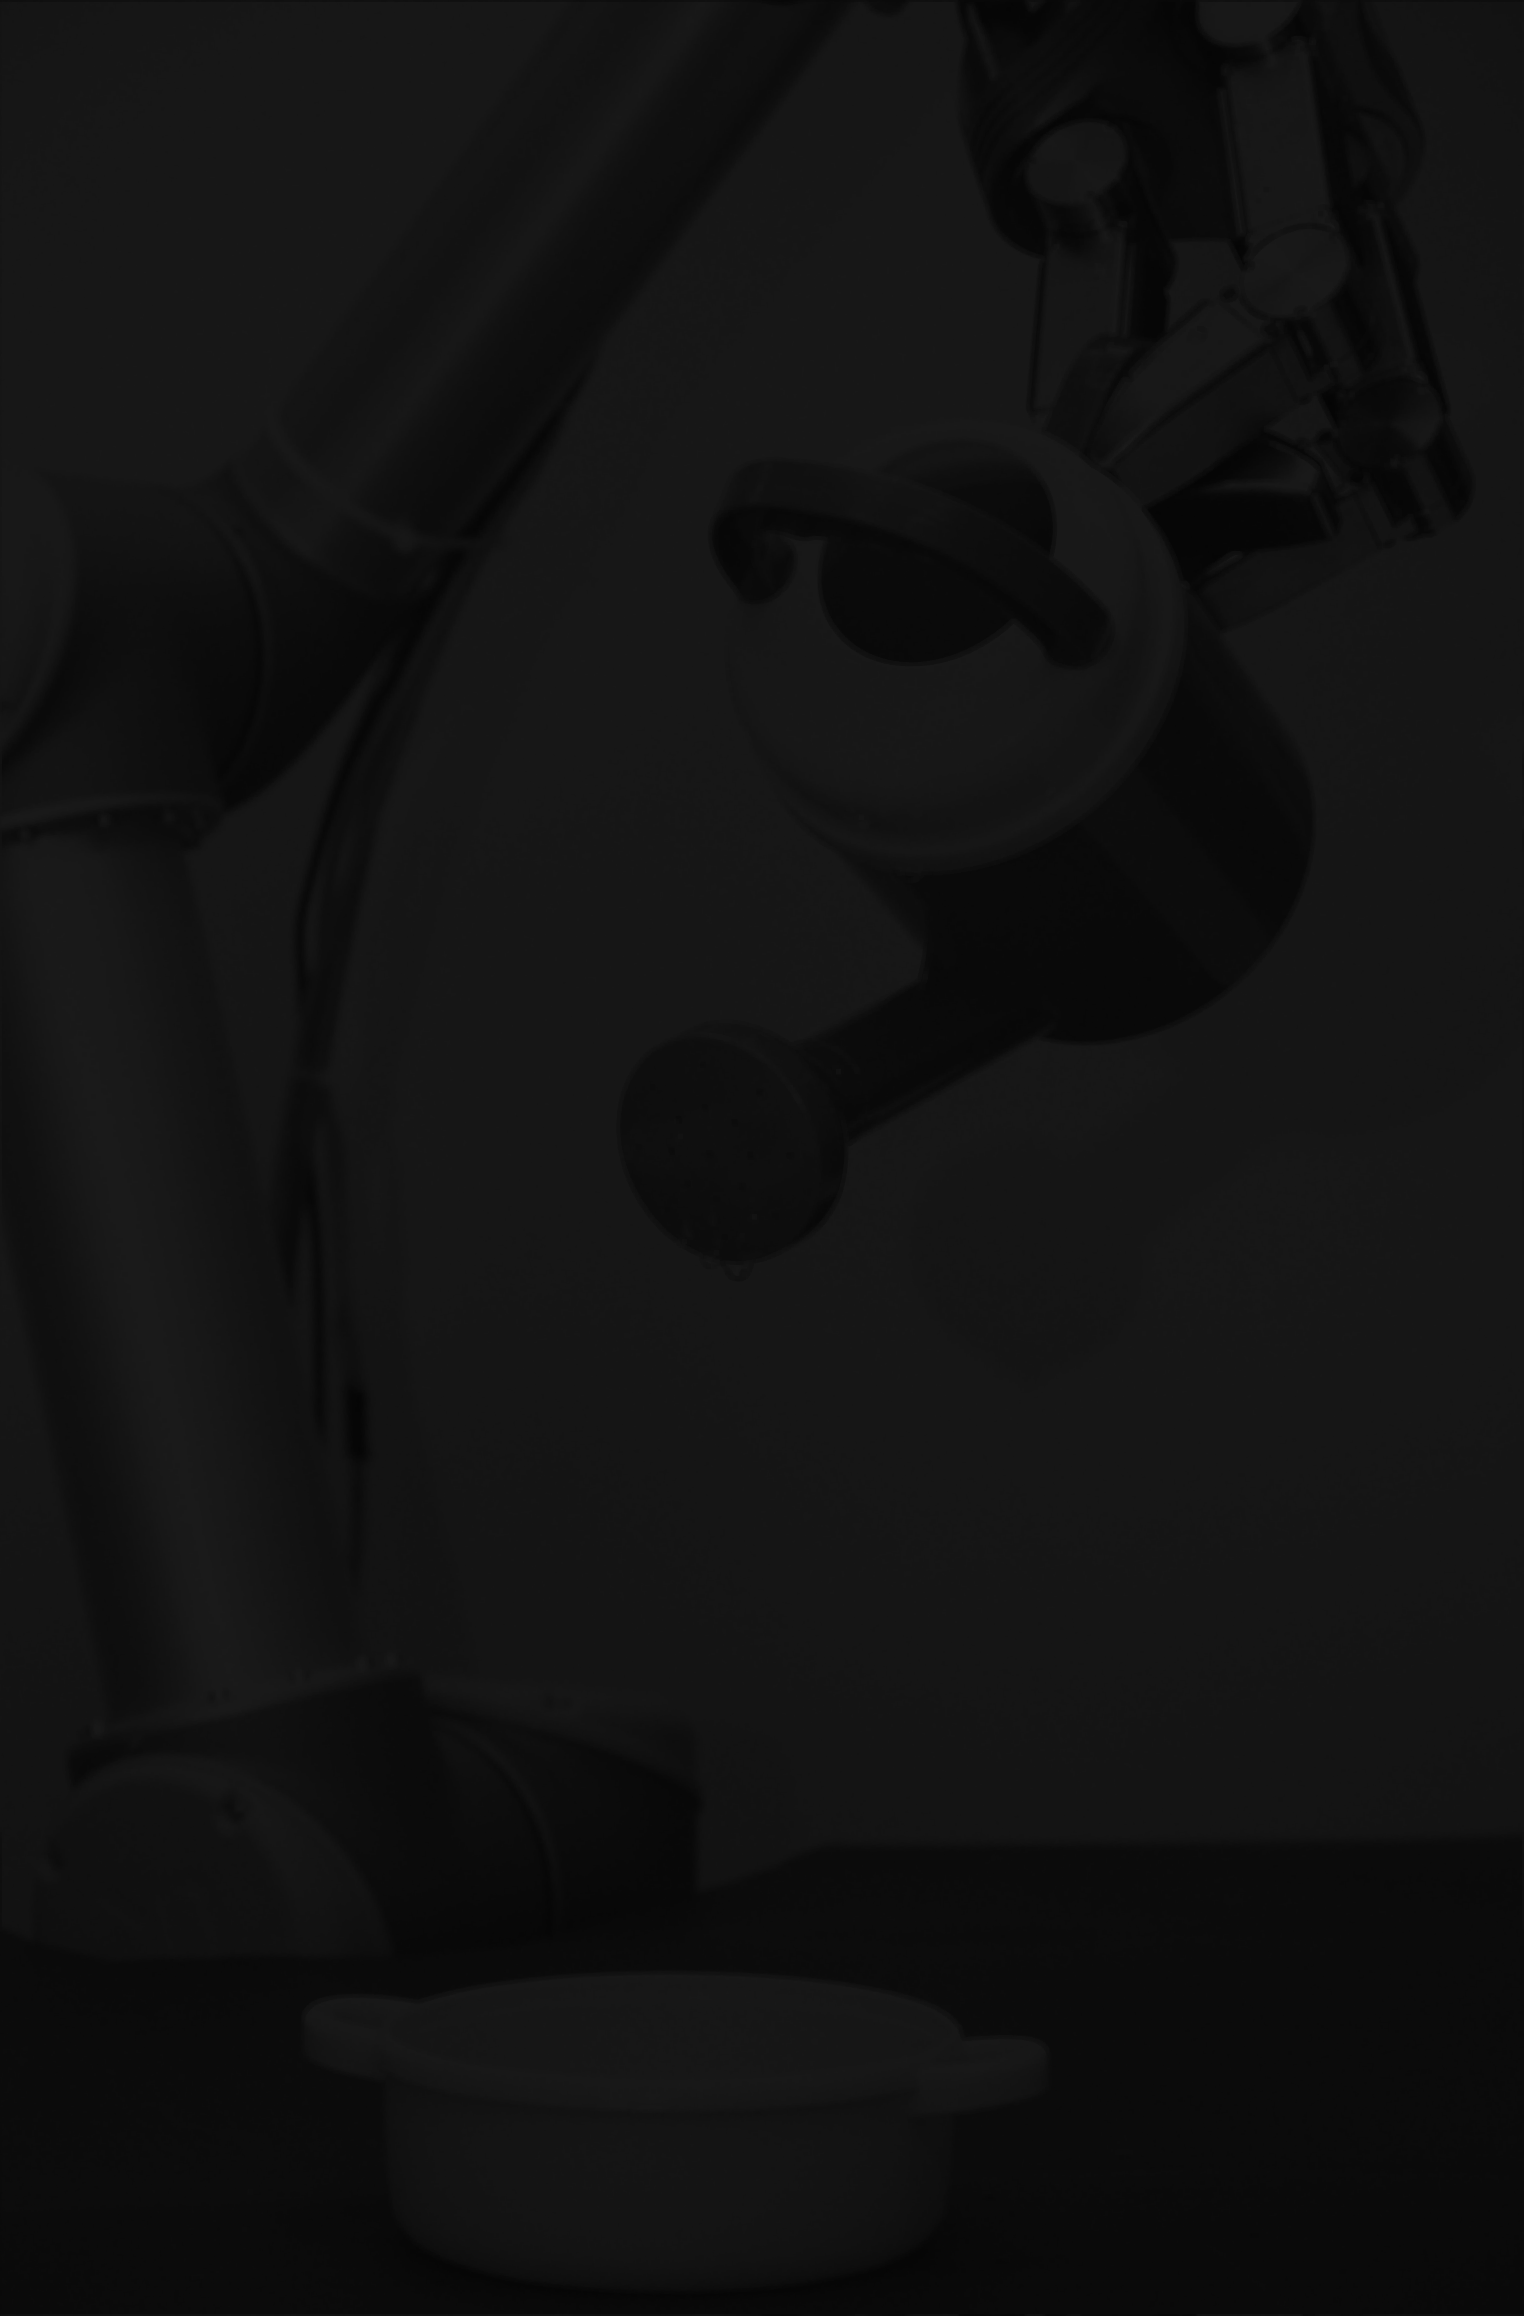
\includegraphics[width=\textwidth]{img3/test/contrast_5_0_1_final_img3.png}
    \end{subfigure}
    \begin{subfigure}[b]{0.1\textwidth}
        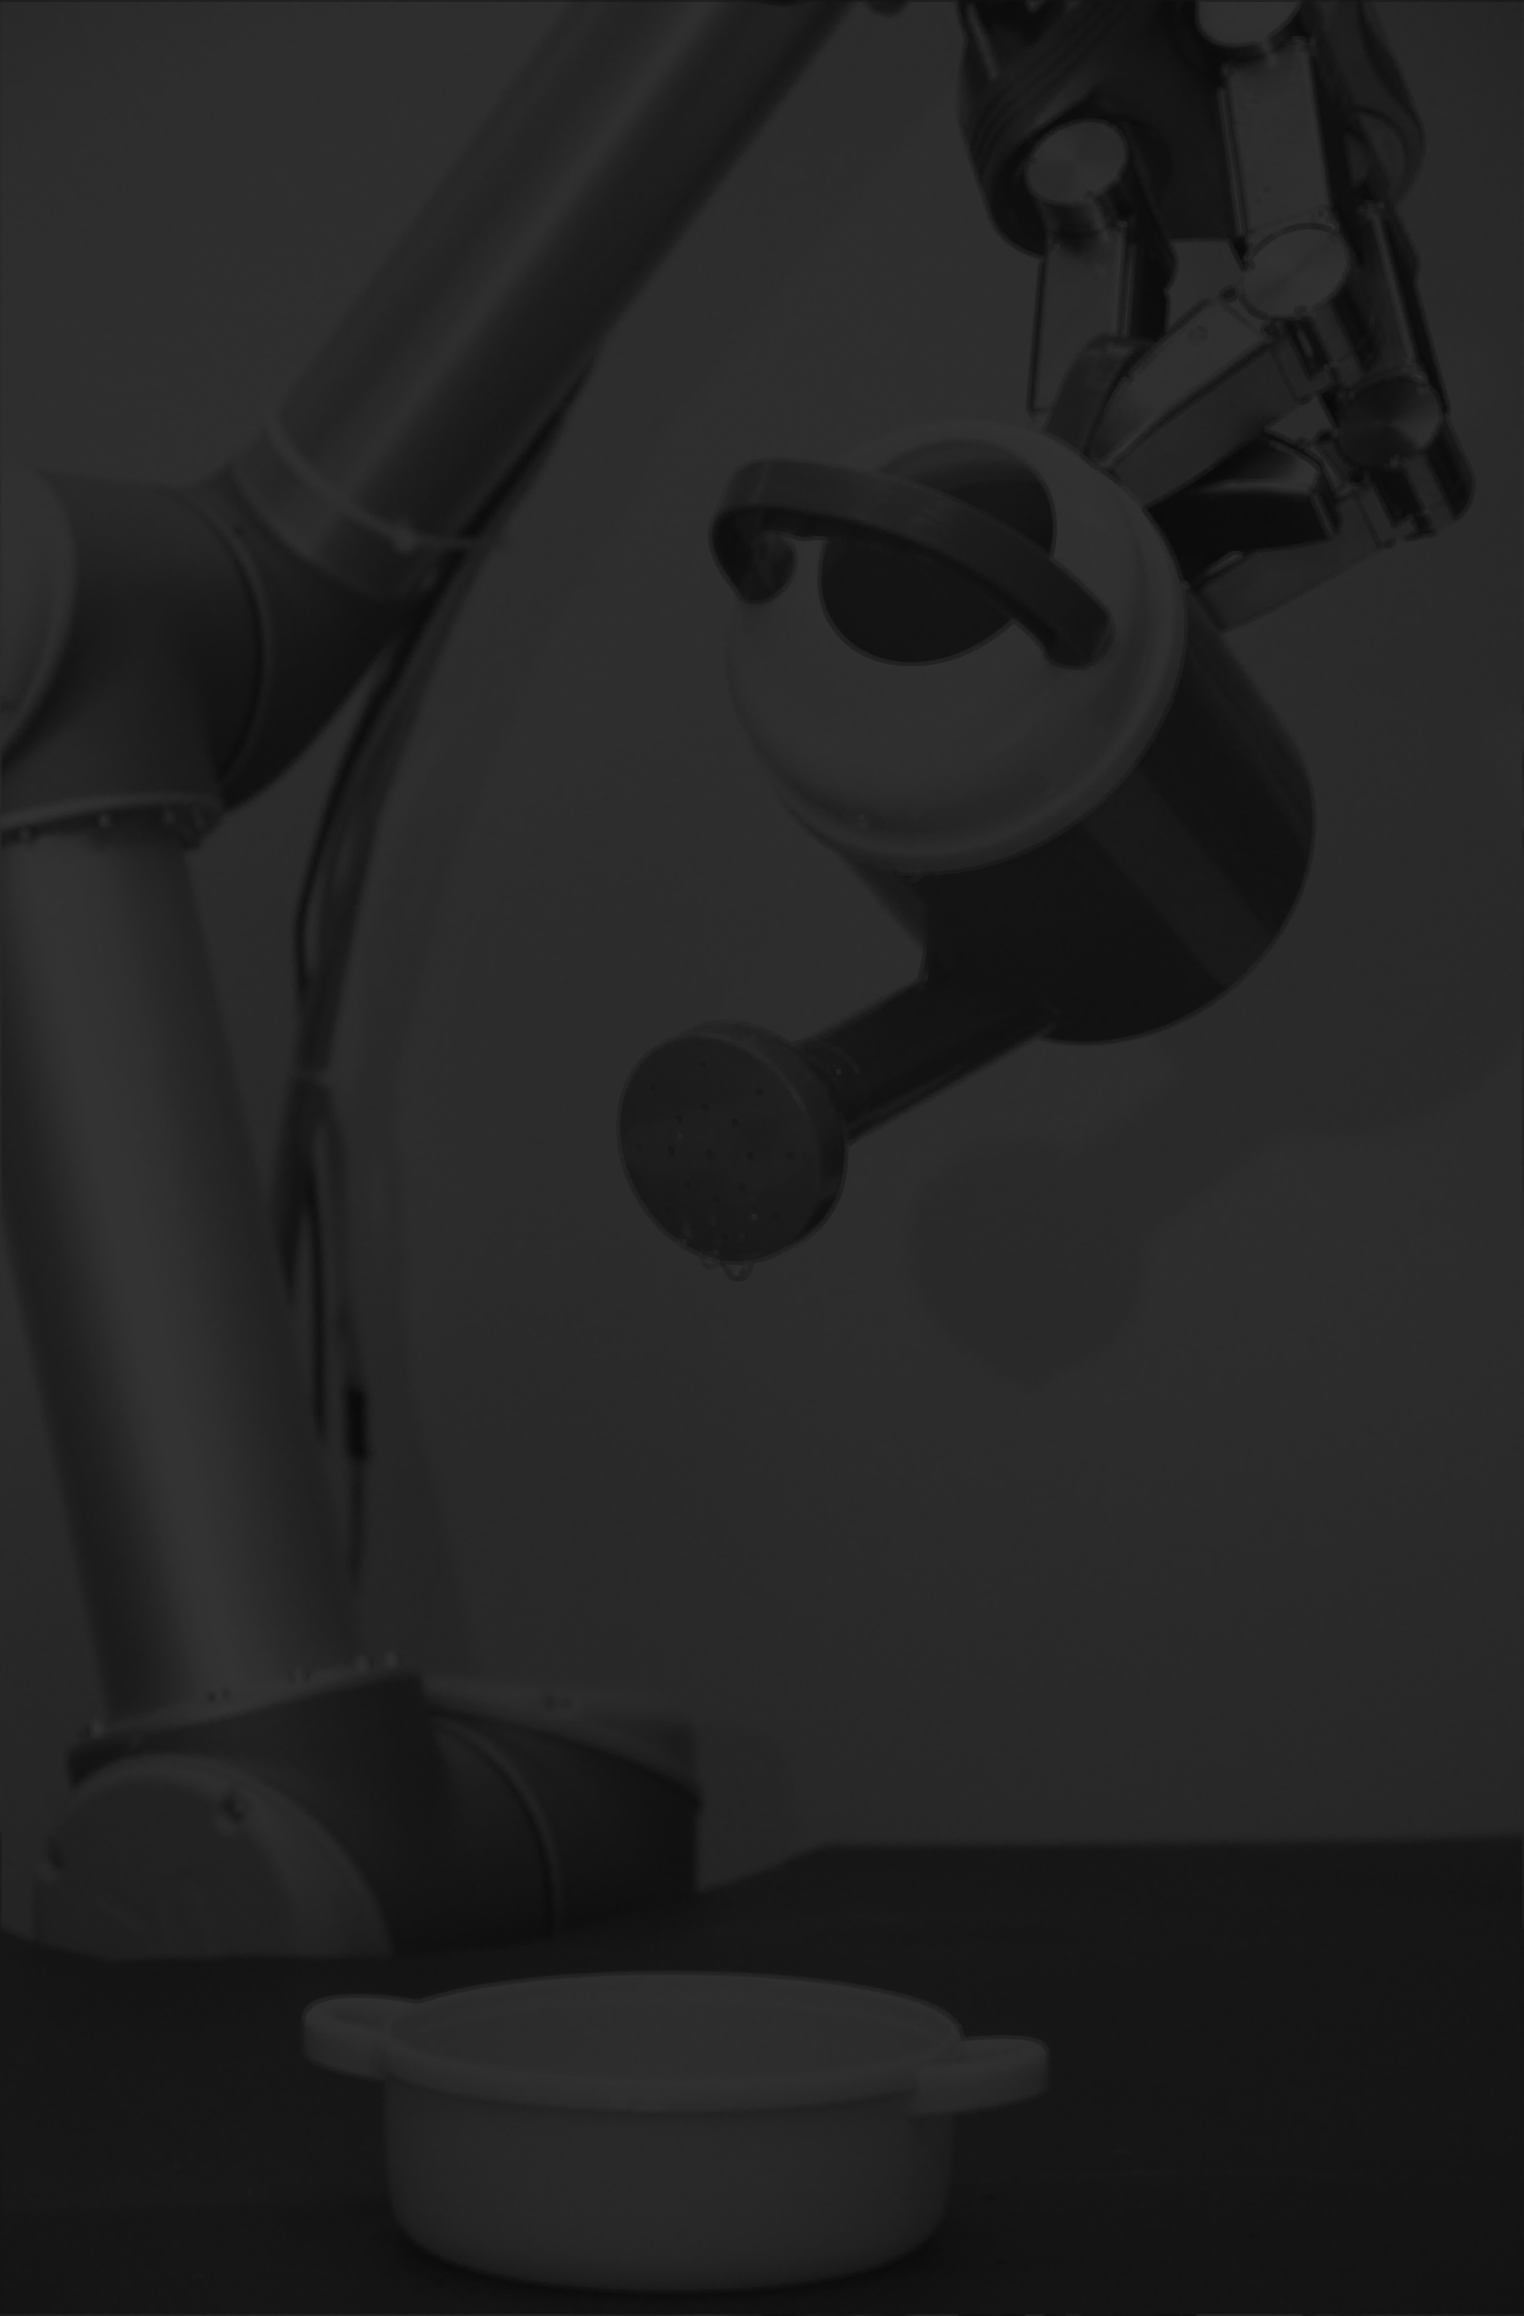
\includegraphics[width=\textwidth]{img3/test/contrast_5_0_2_final_img3.png}
    \end{subfigure}
    \begin{subfigure}[b]{0.1\textwidth}
        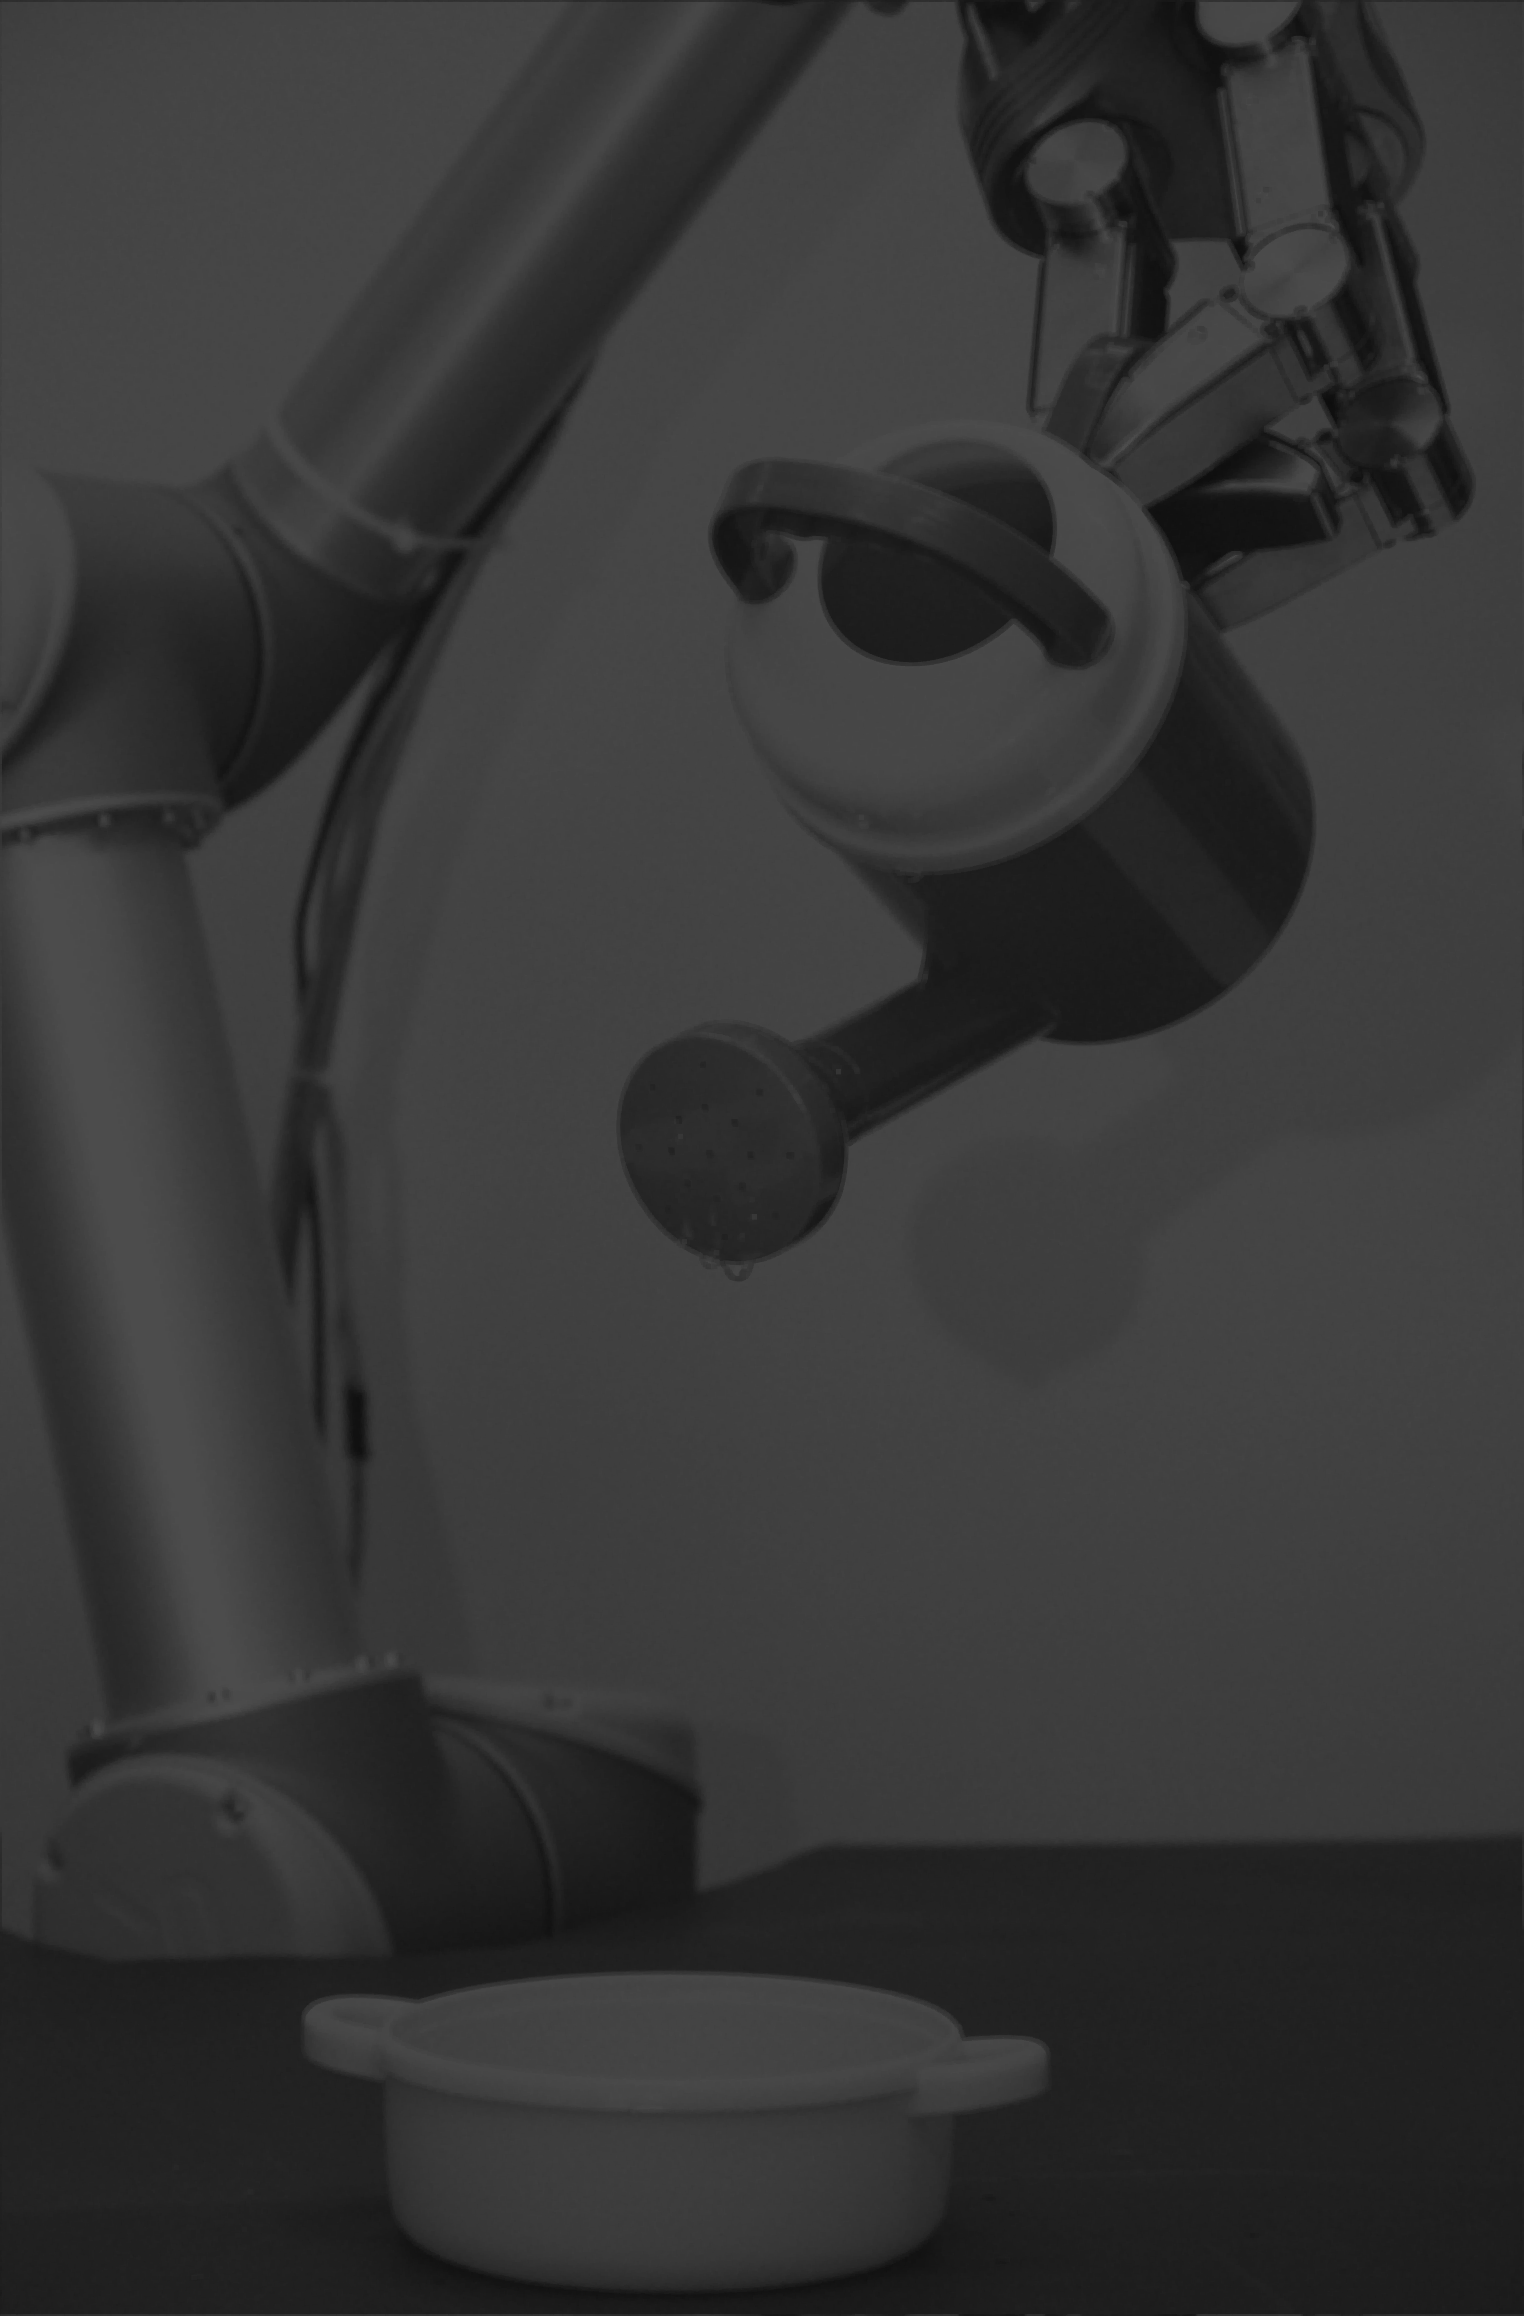
\includegraphics[width=\textwidth]{img3/test/contrast_5_0_3_final_img3.png}
    \end{subfigure}
    \begin{subfigure}[b]{0.1\textwidth}
        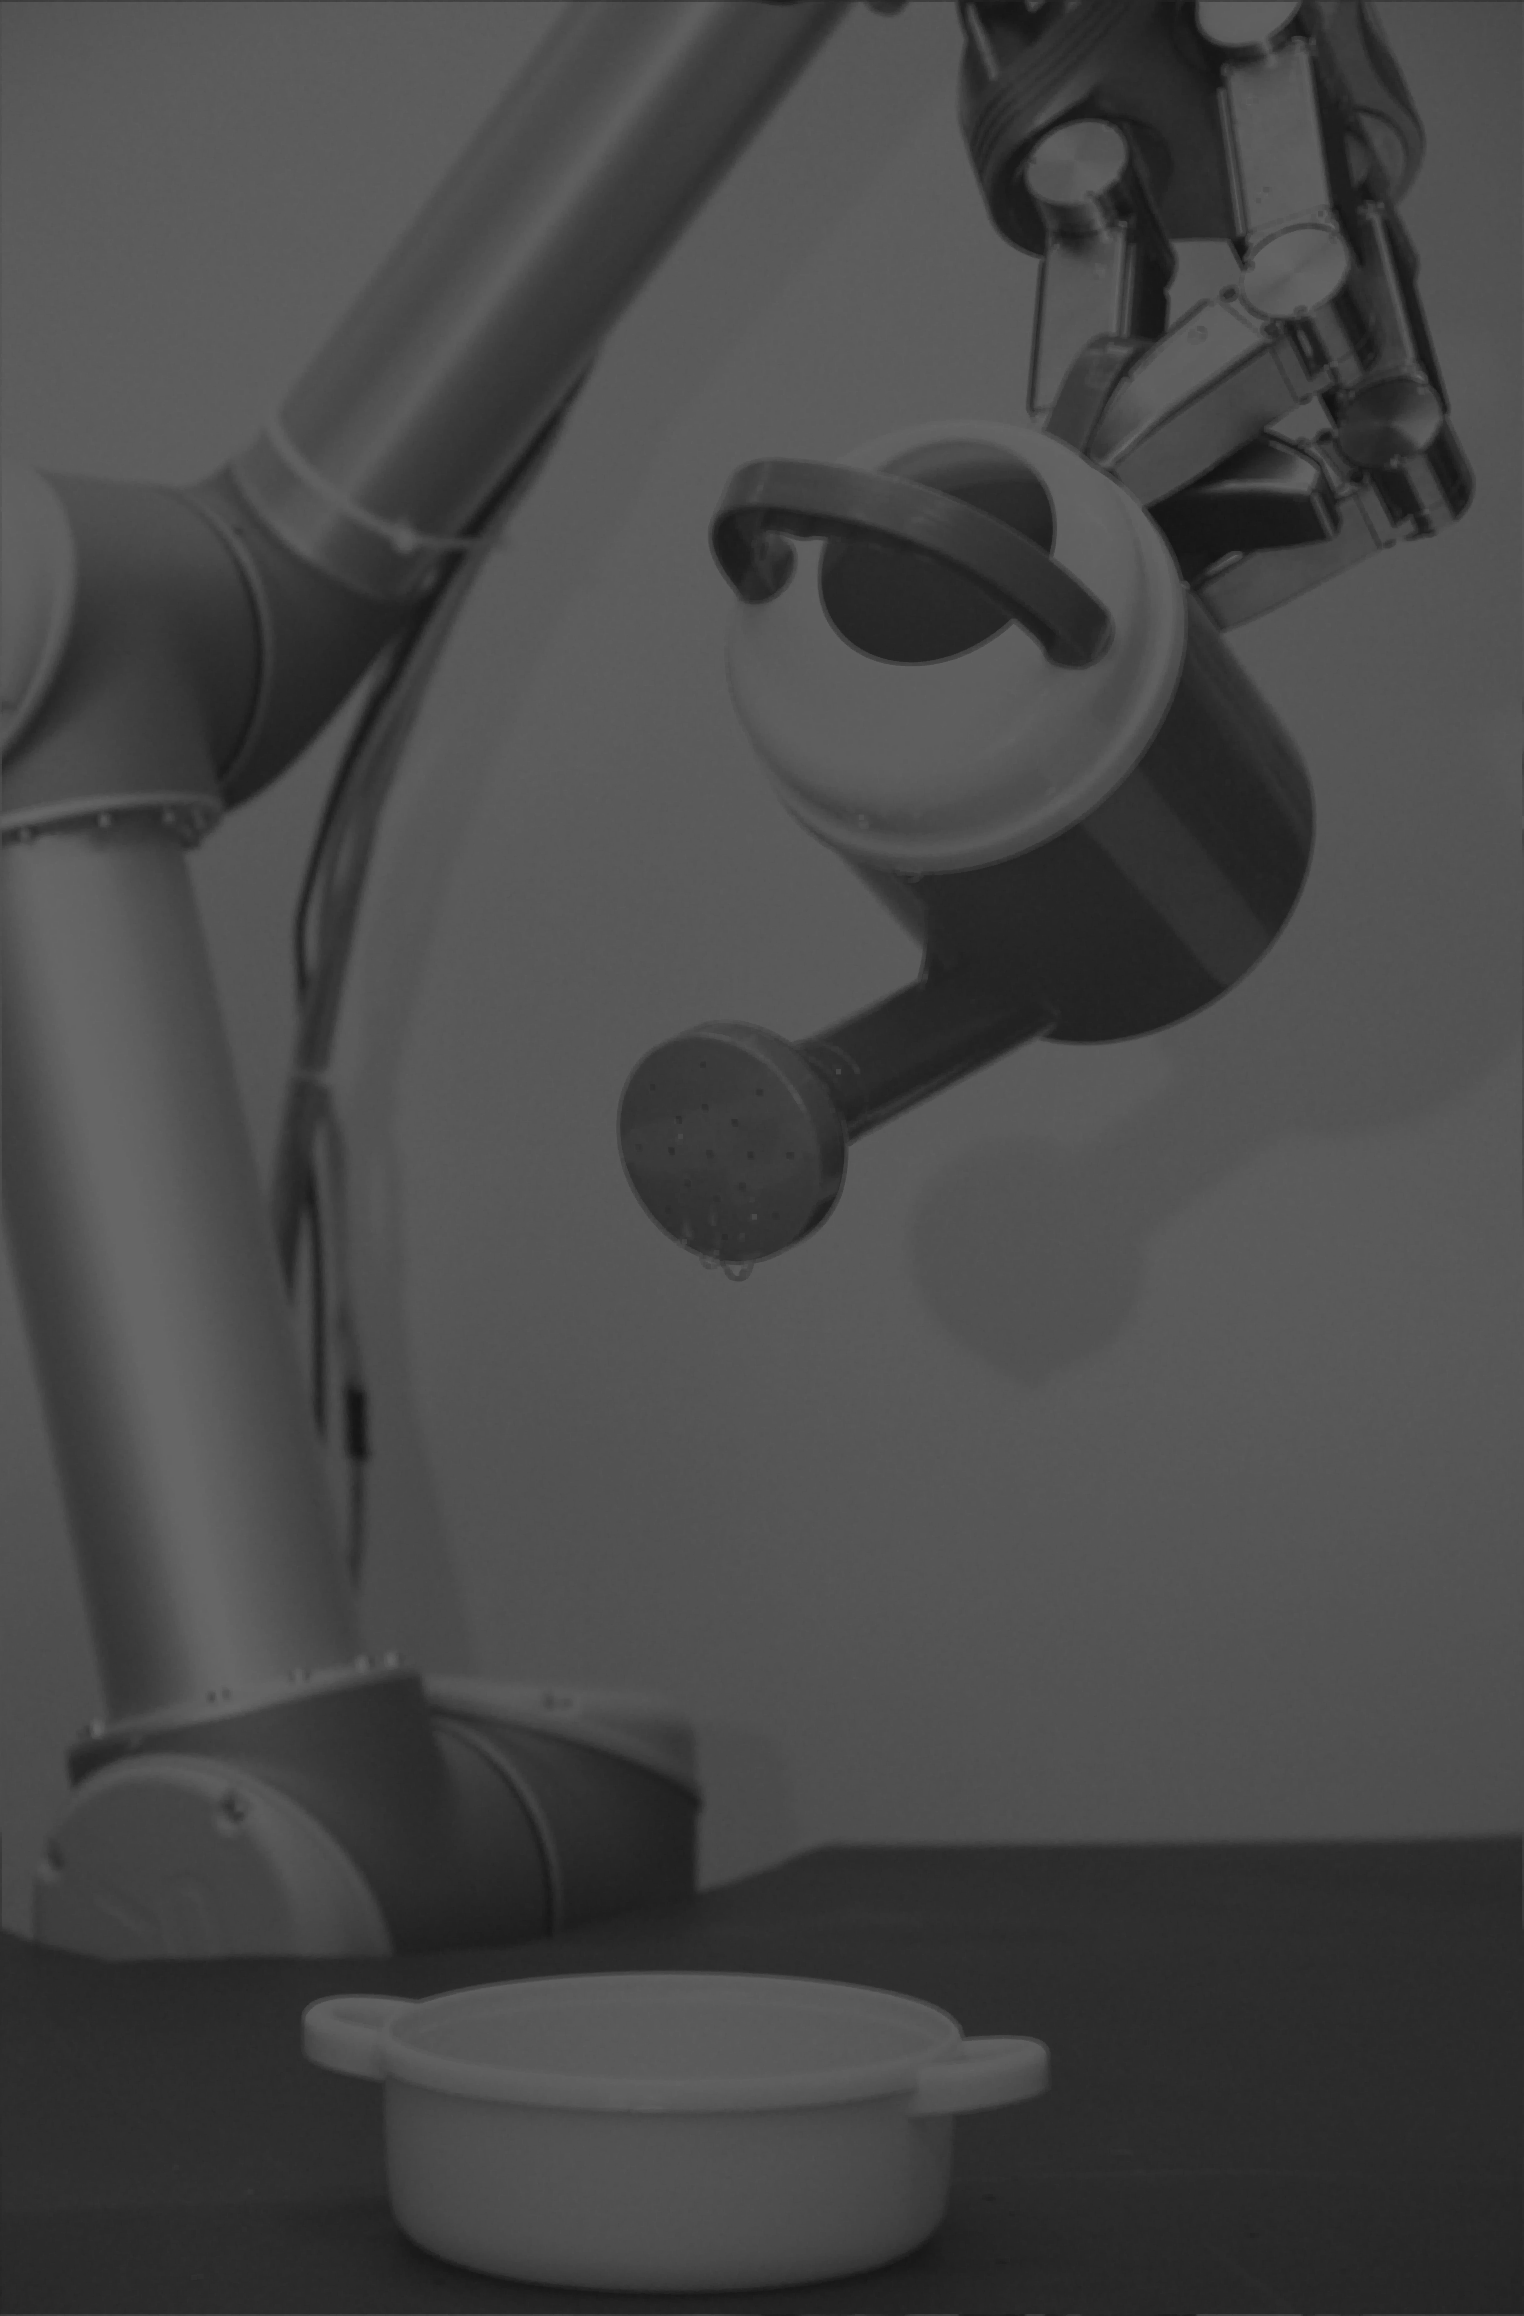
\includegraphics[width=\textwidth]{img3/test/contrast_5_0_4_final_img3.png}
    \end{subfigure}
    \begin{subfigure}[b]{0.1\textwidth}
        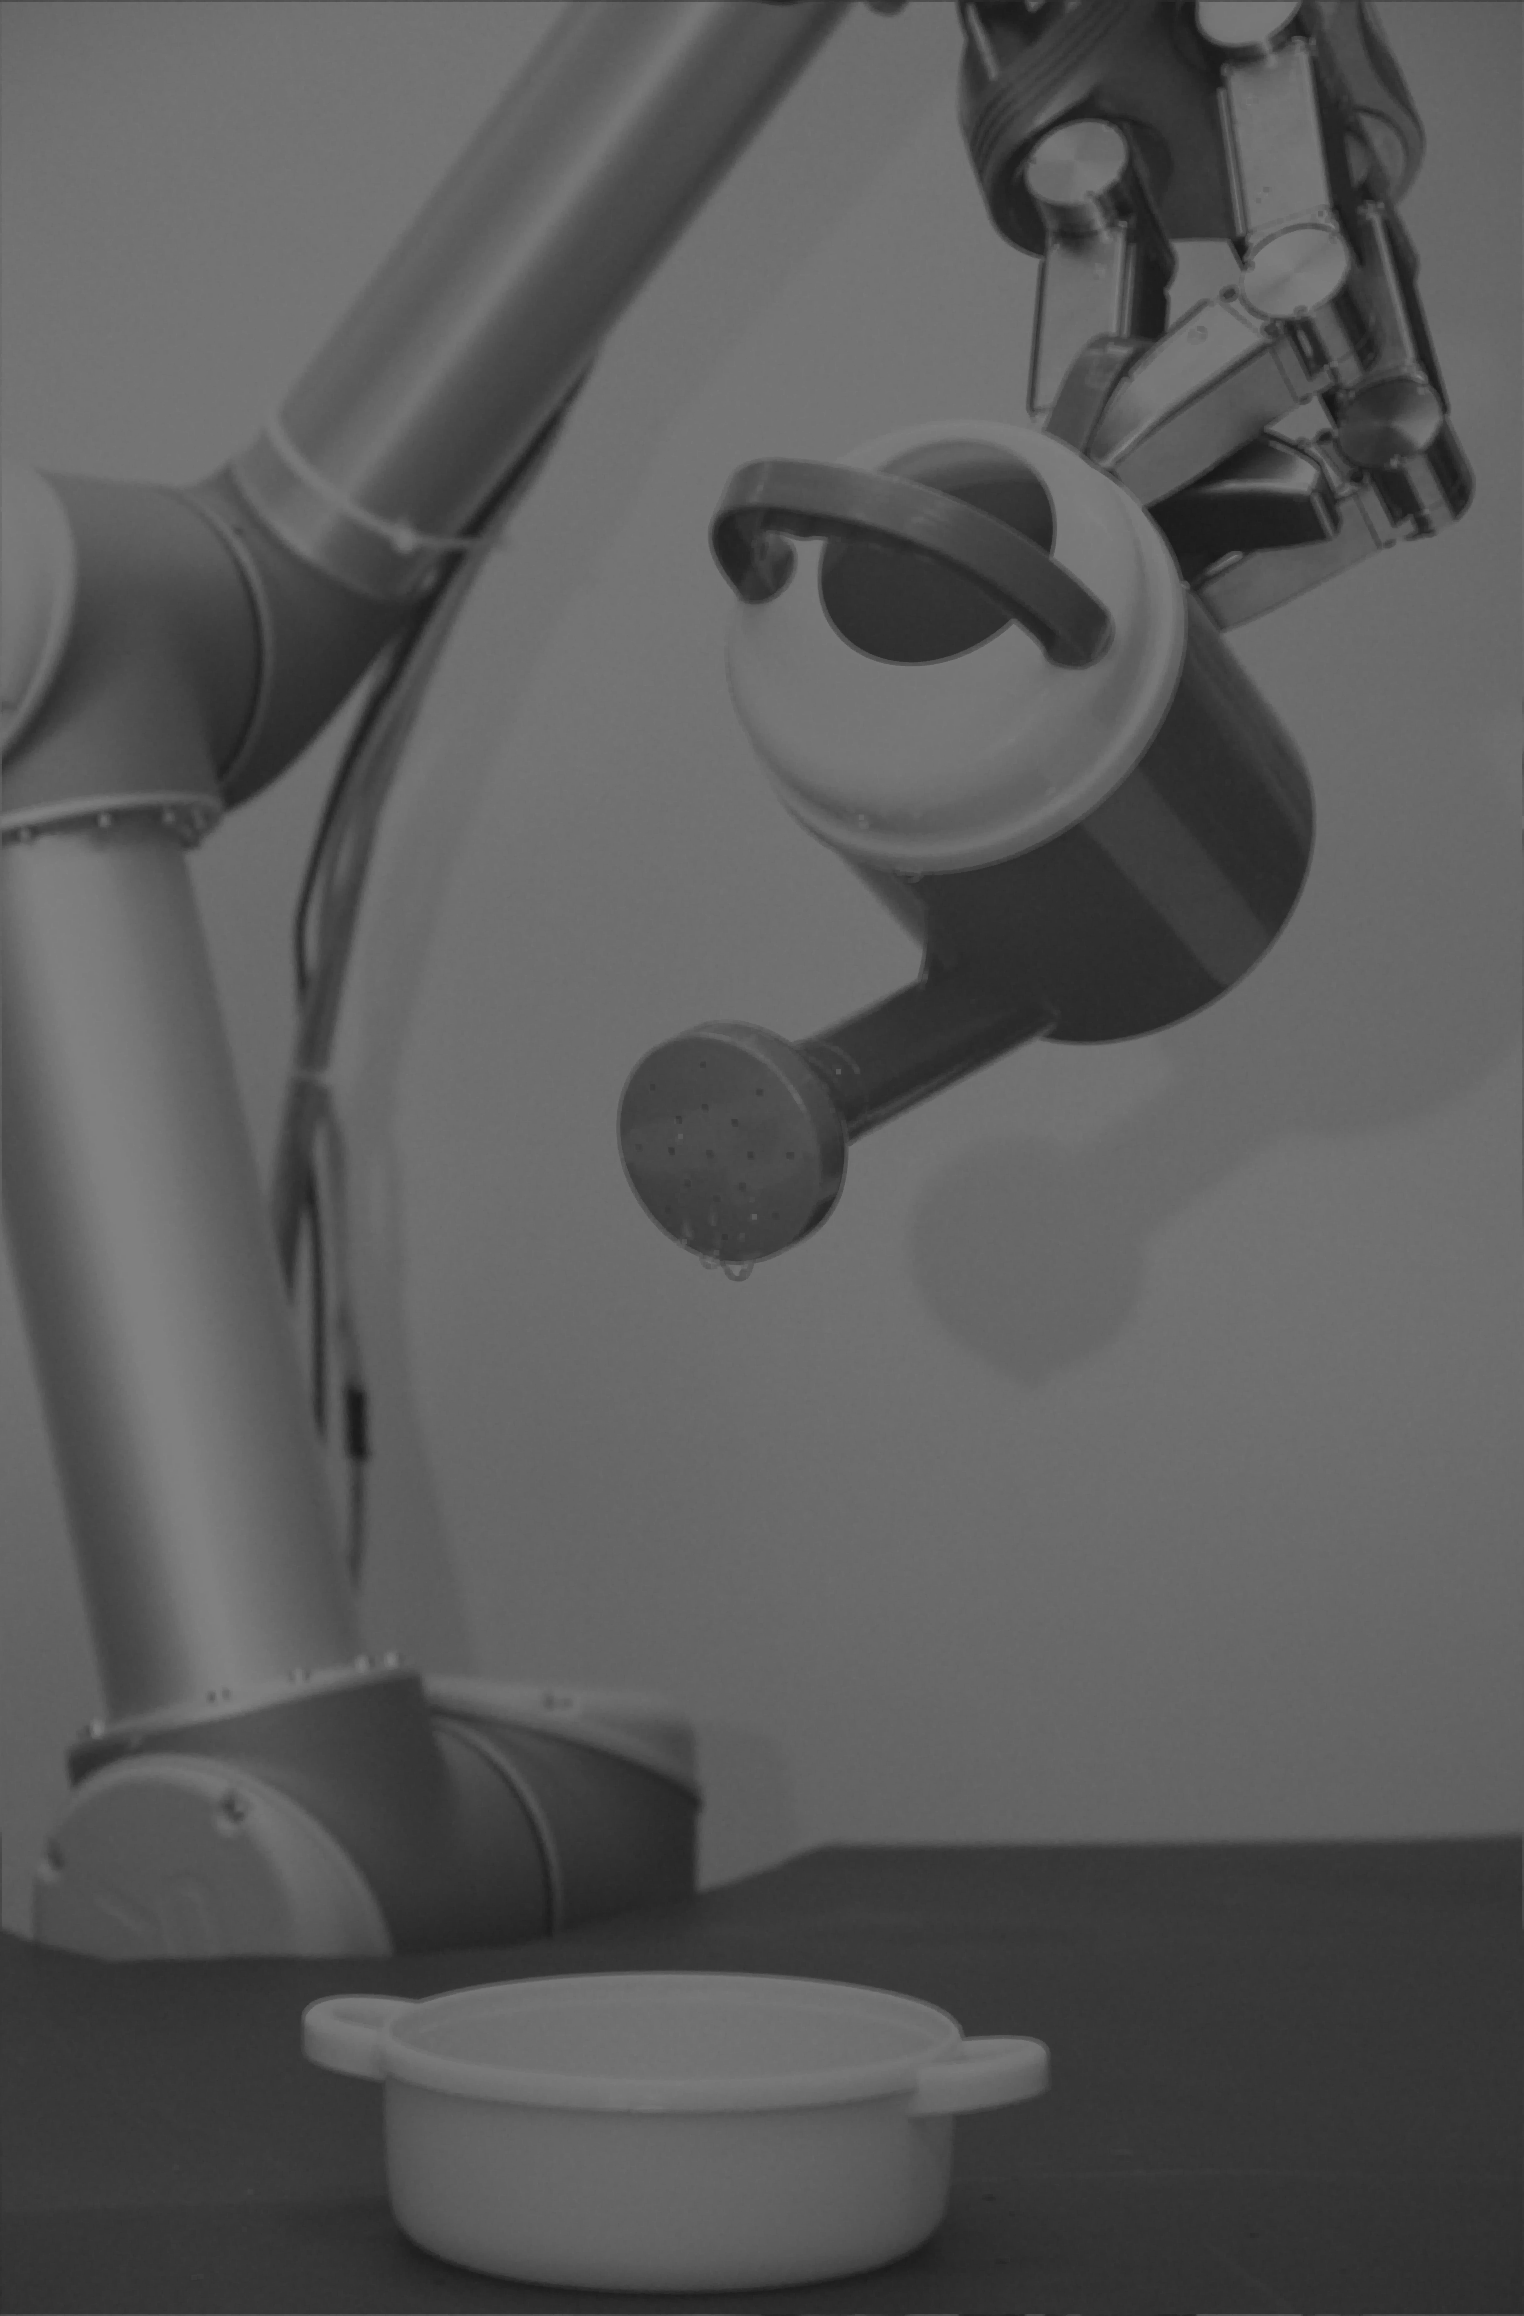
\includegraphics[width=\textwidth]{img3/test/contrast_5_0_5_final_img3.png}
    \end{subfigure}
    \begin{subfigure}[b]{0.1\textwidth}
        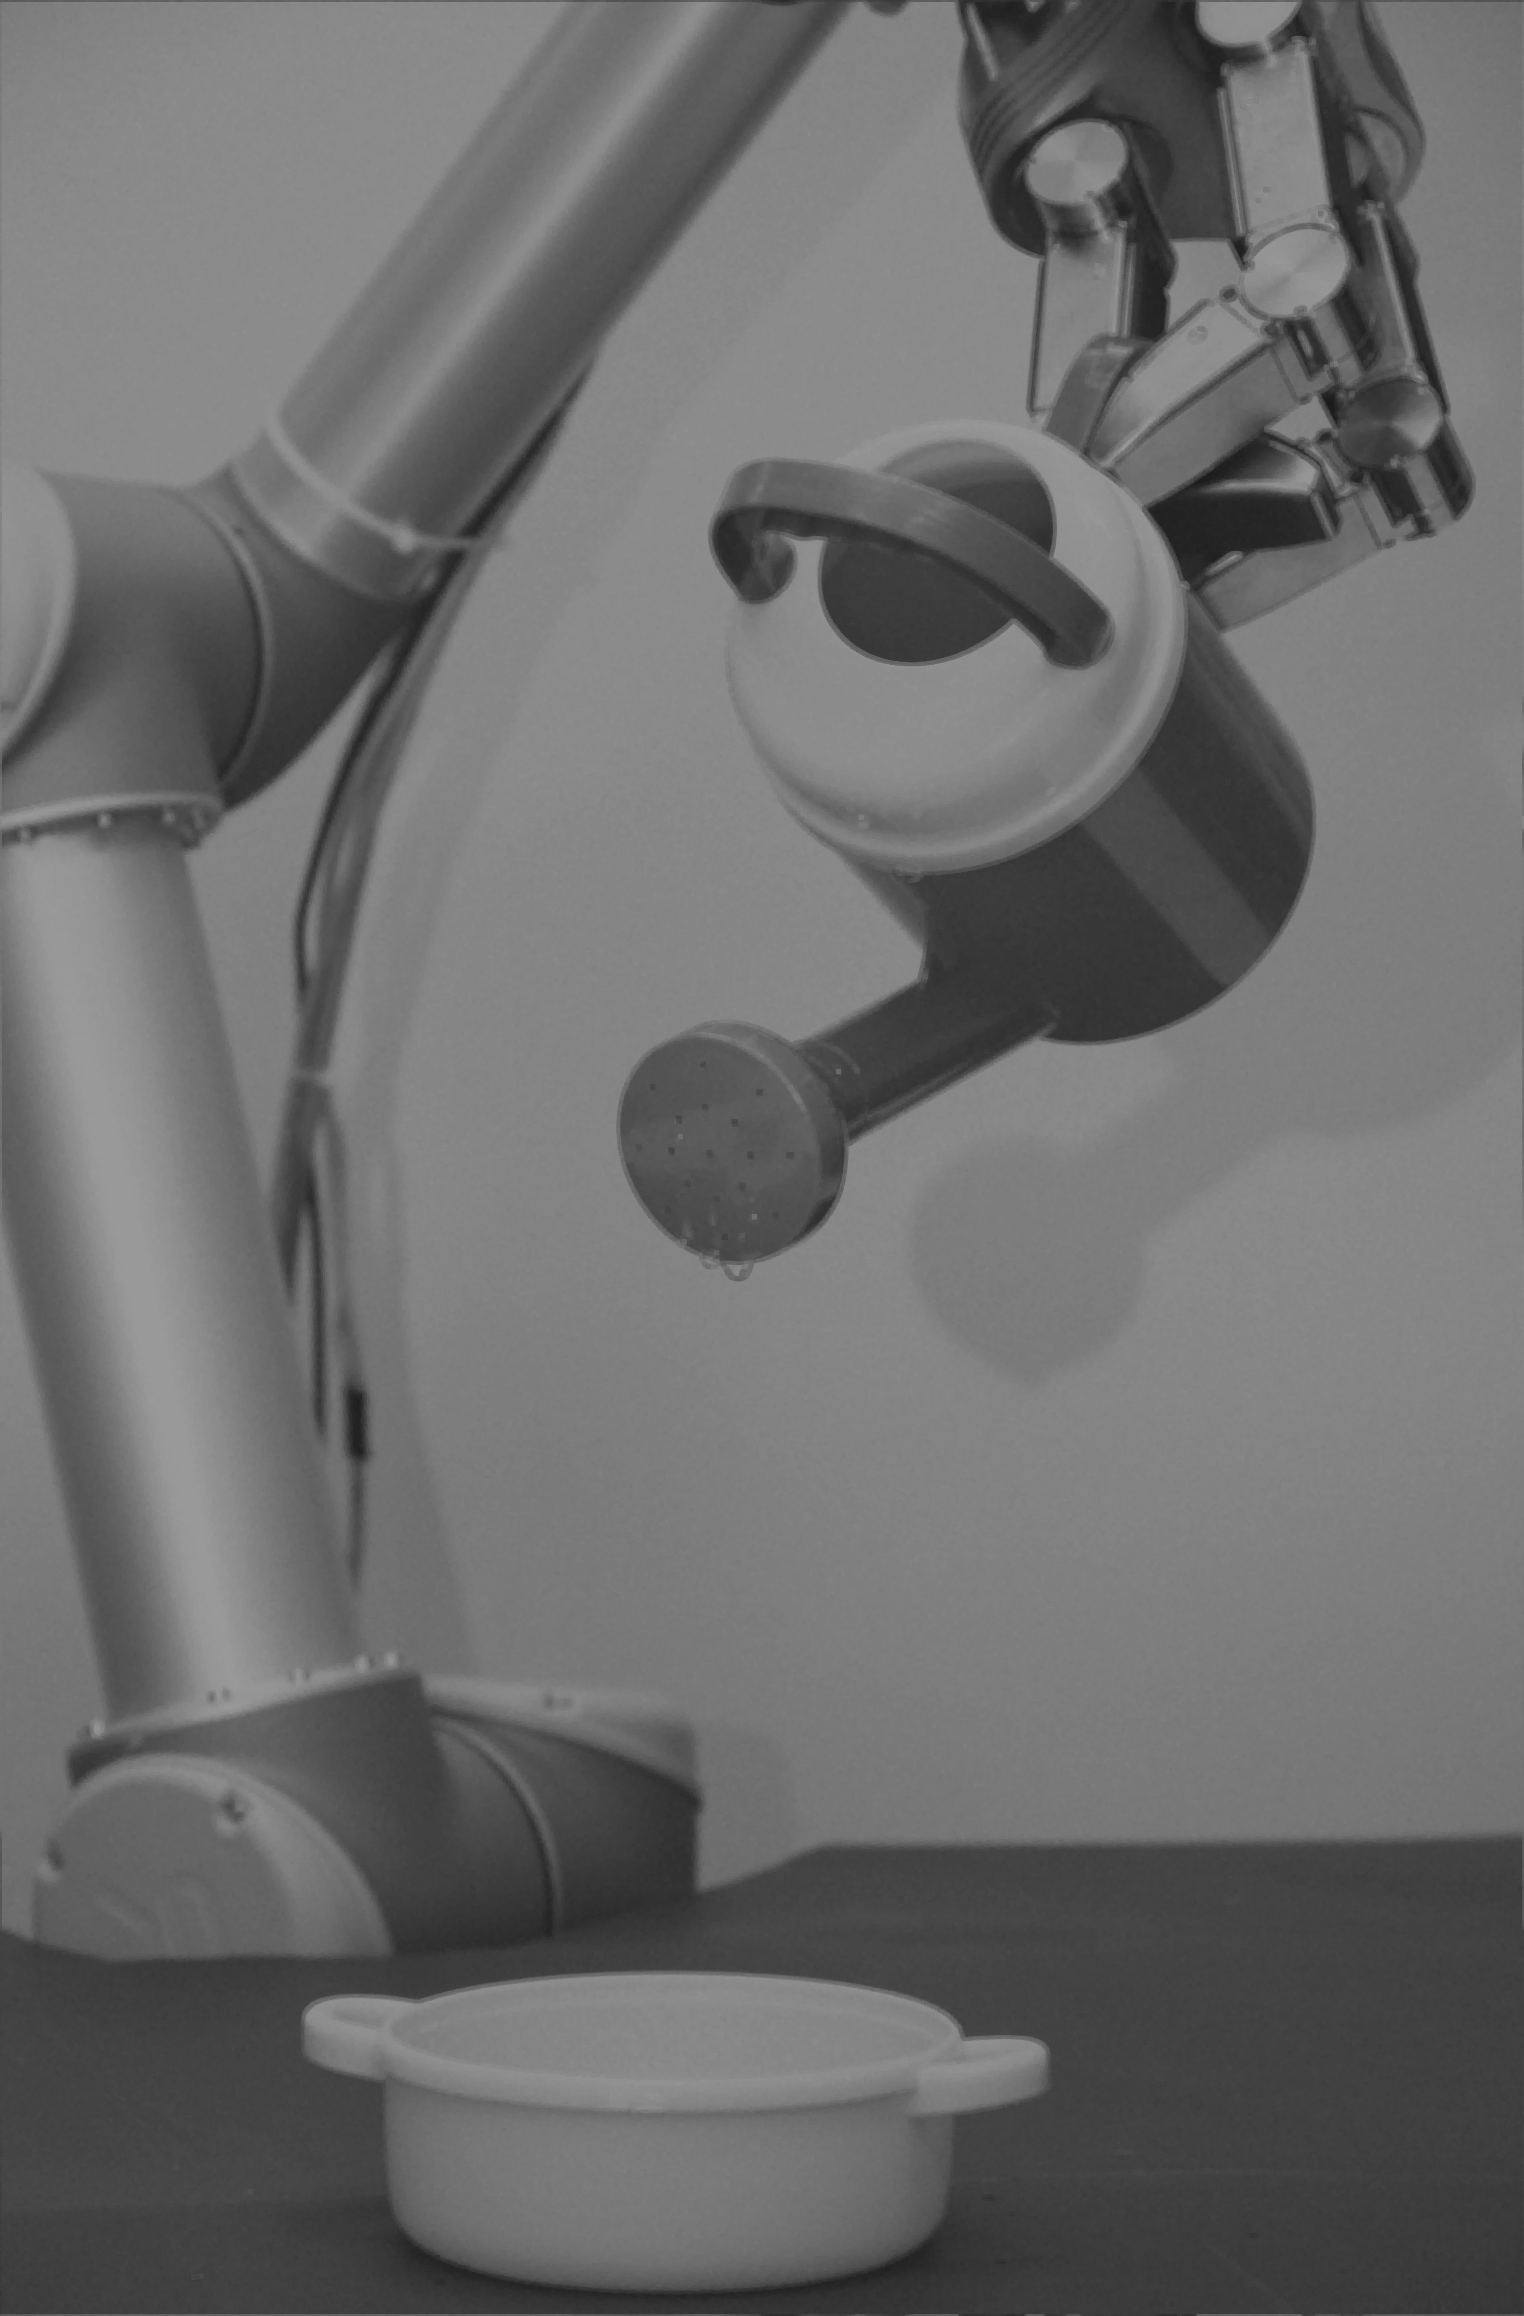
\includegraphics[width=\textwidth]{img3/test/contrast_5_0_6_final_img3.png}
    \end{subfigure}
    \begin{subfigure}[b]{0.1\textwidth}
        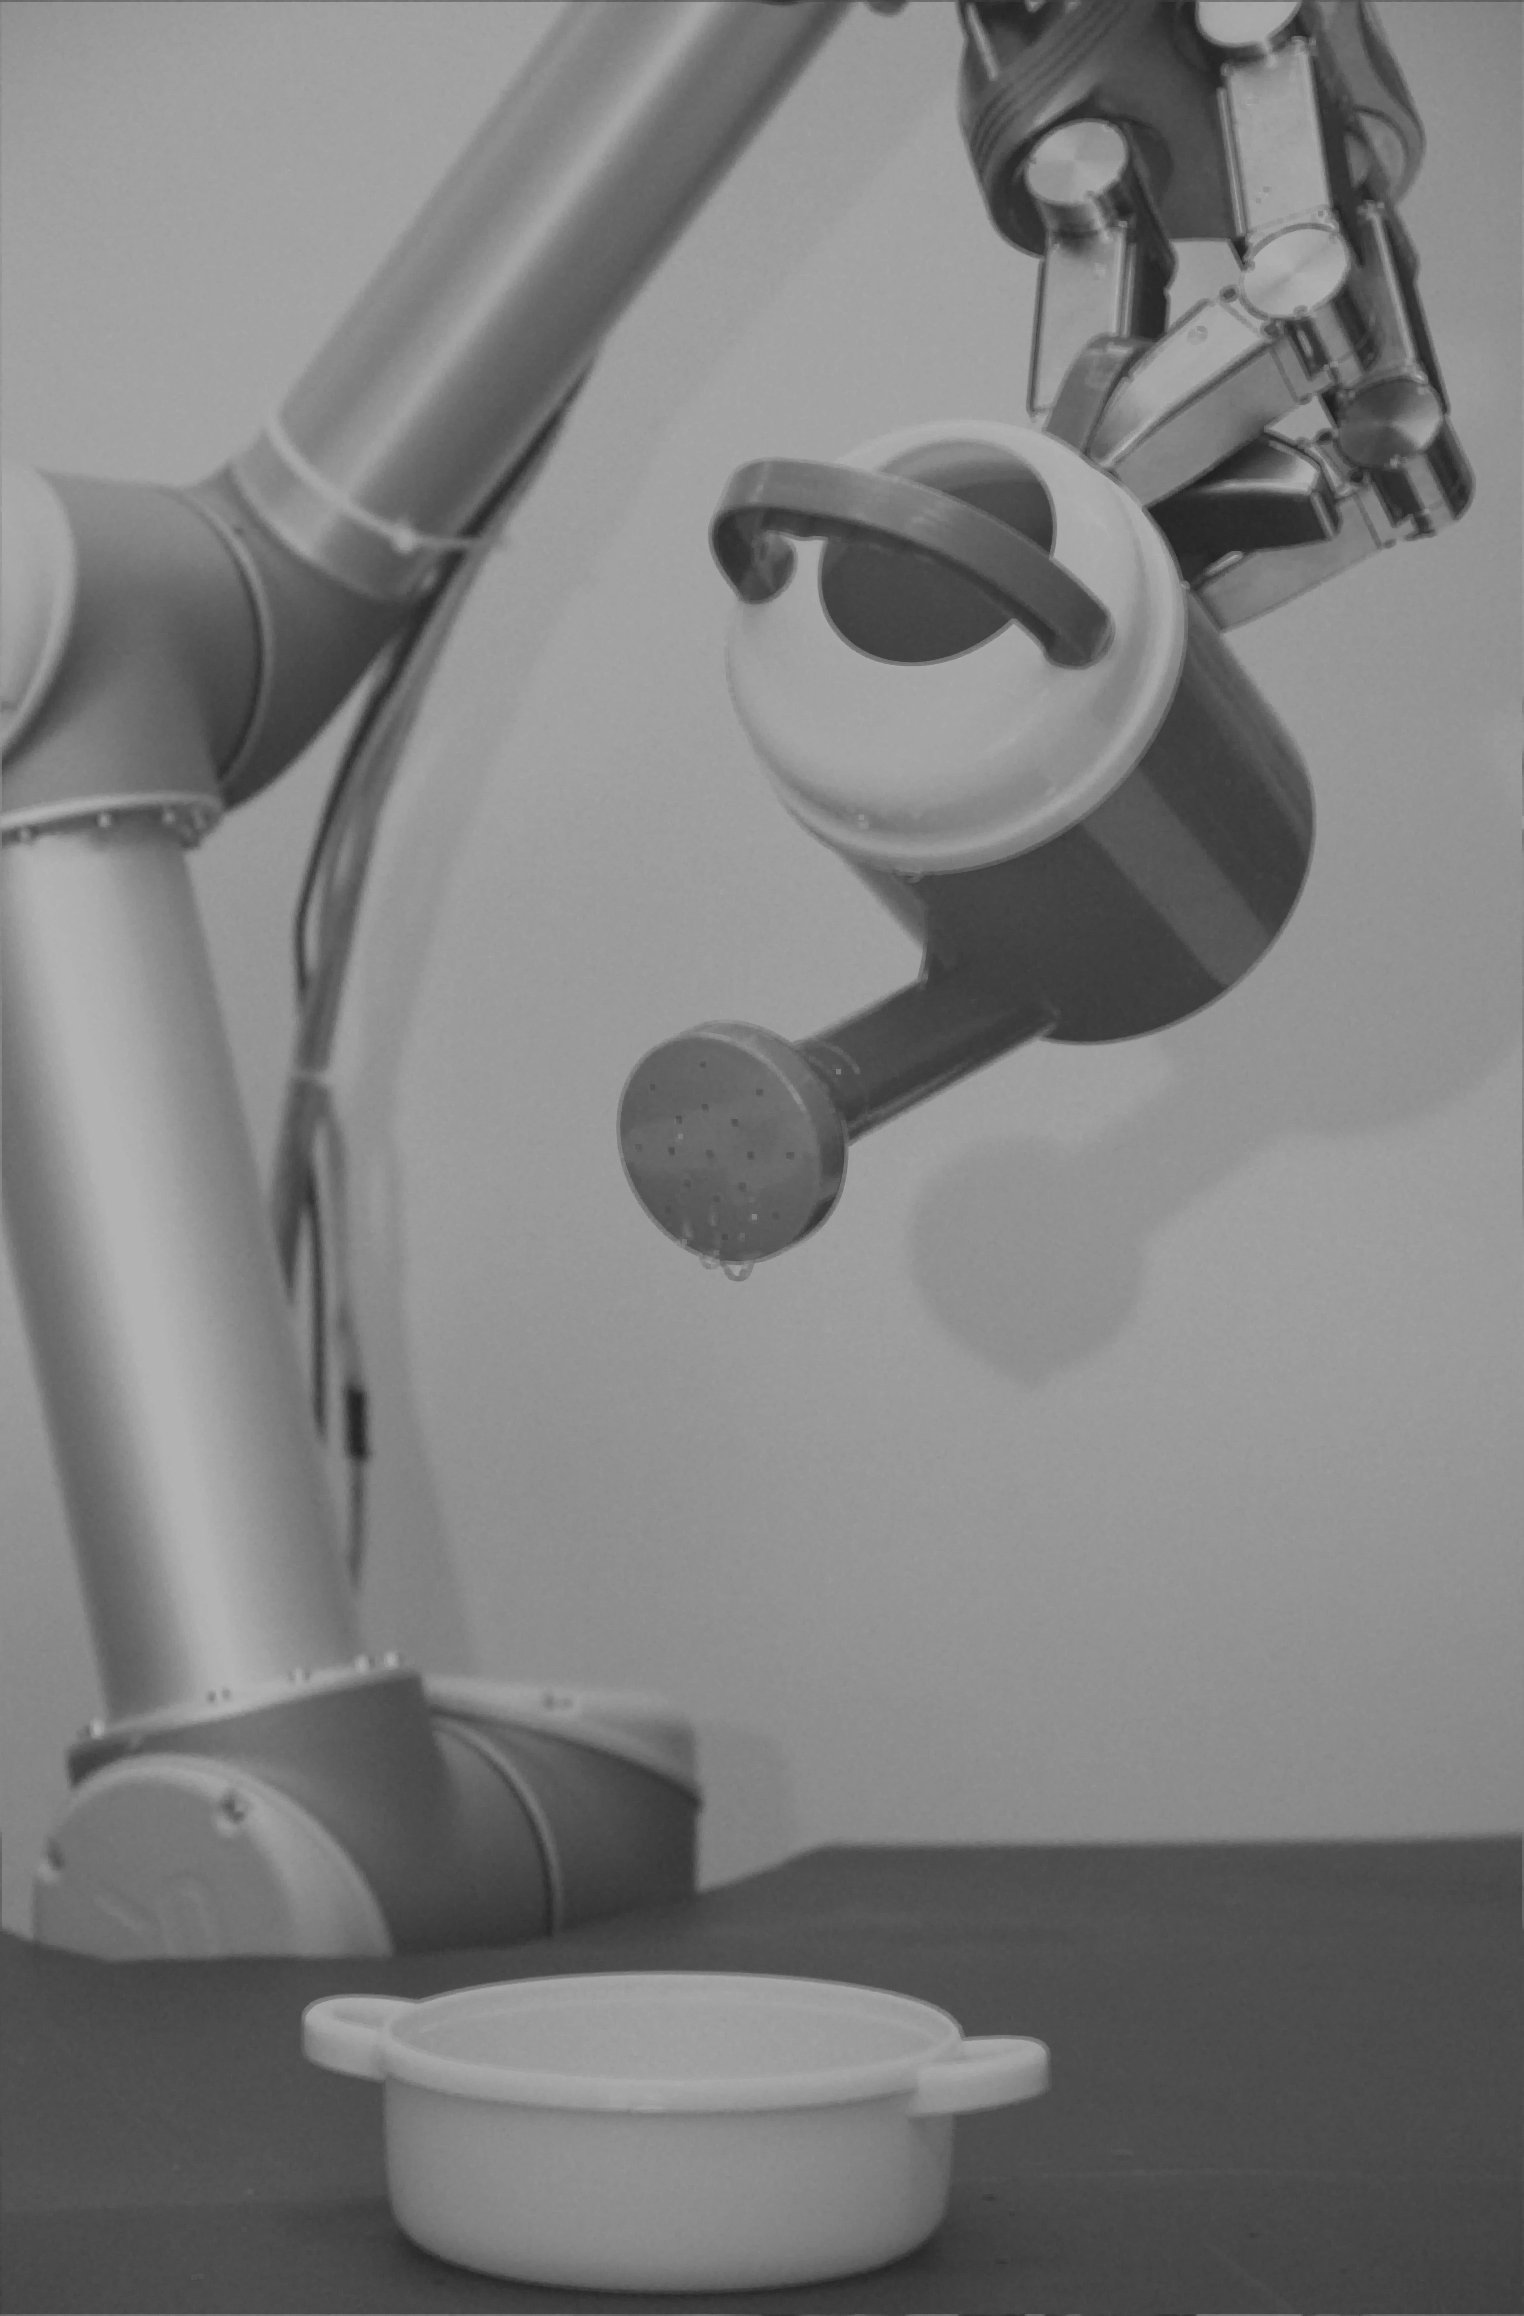
\includegraphics[width=\textwidth]{img3/test/contrast_5_0_7_final_img3.png}
    \end{subfigure}
    \begin{subfigure}[b]{0.1\textwidth}
        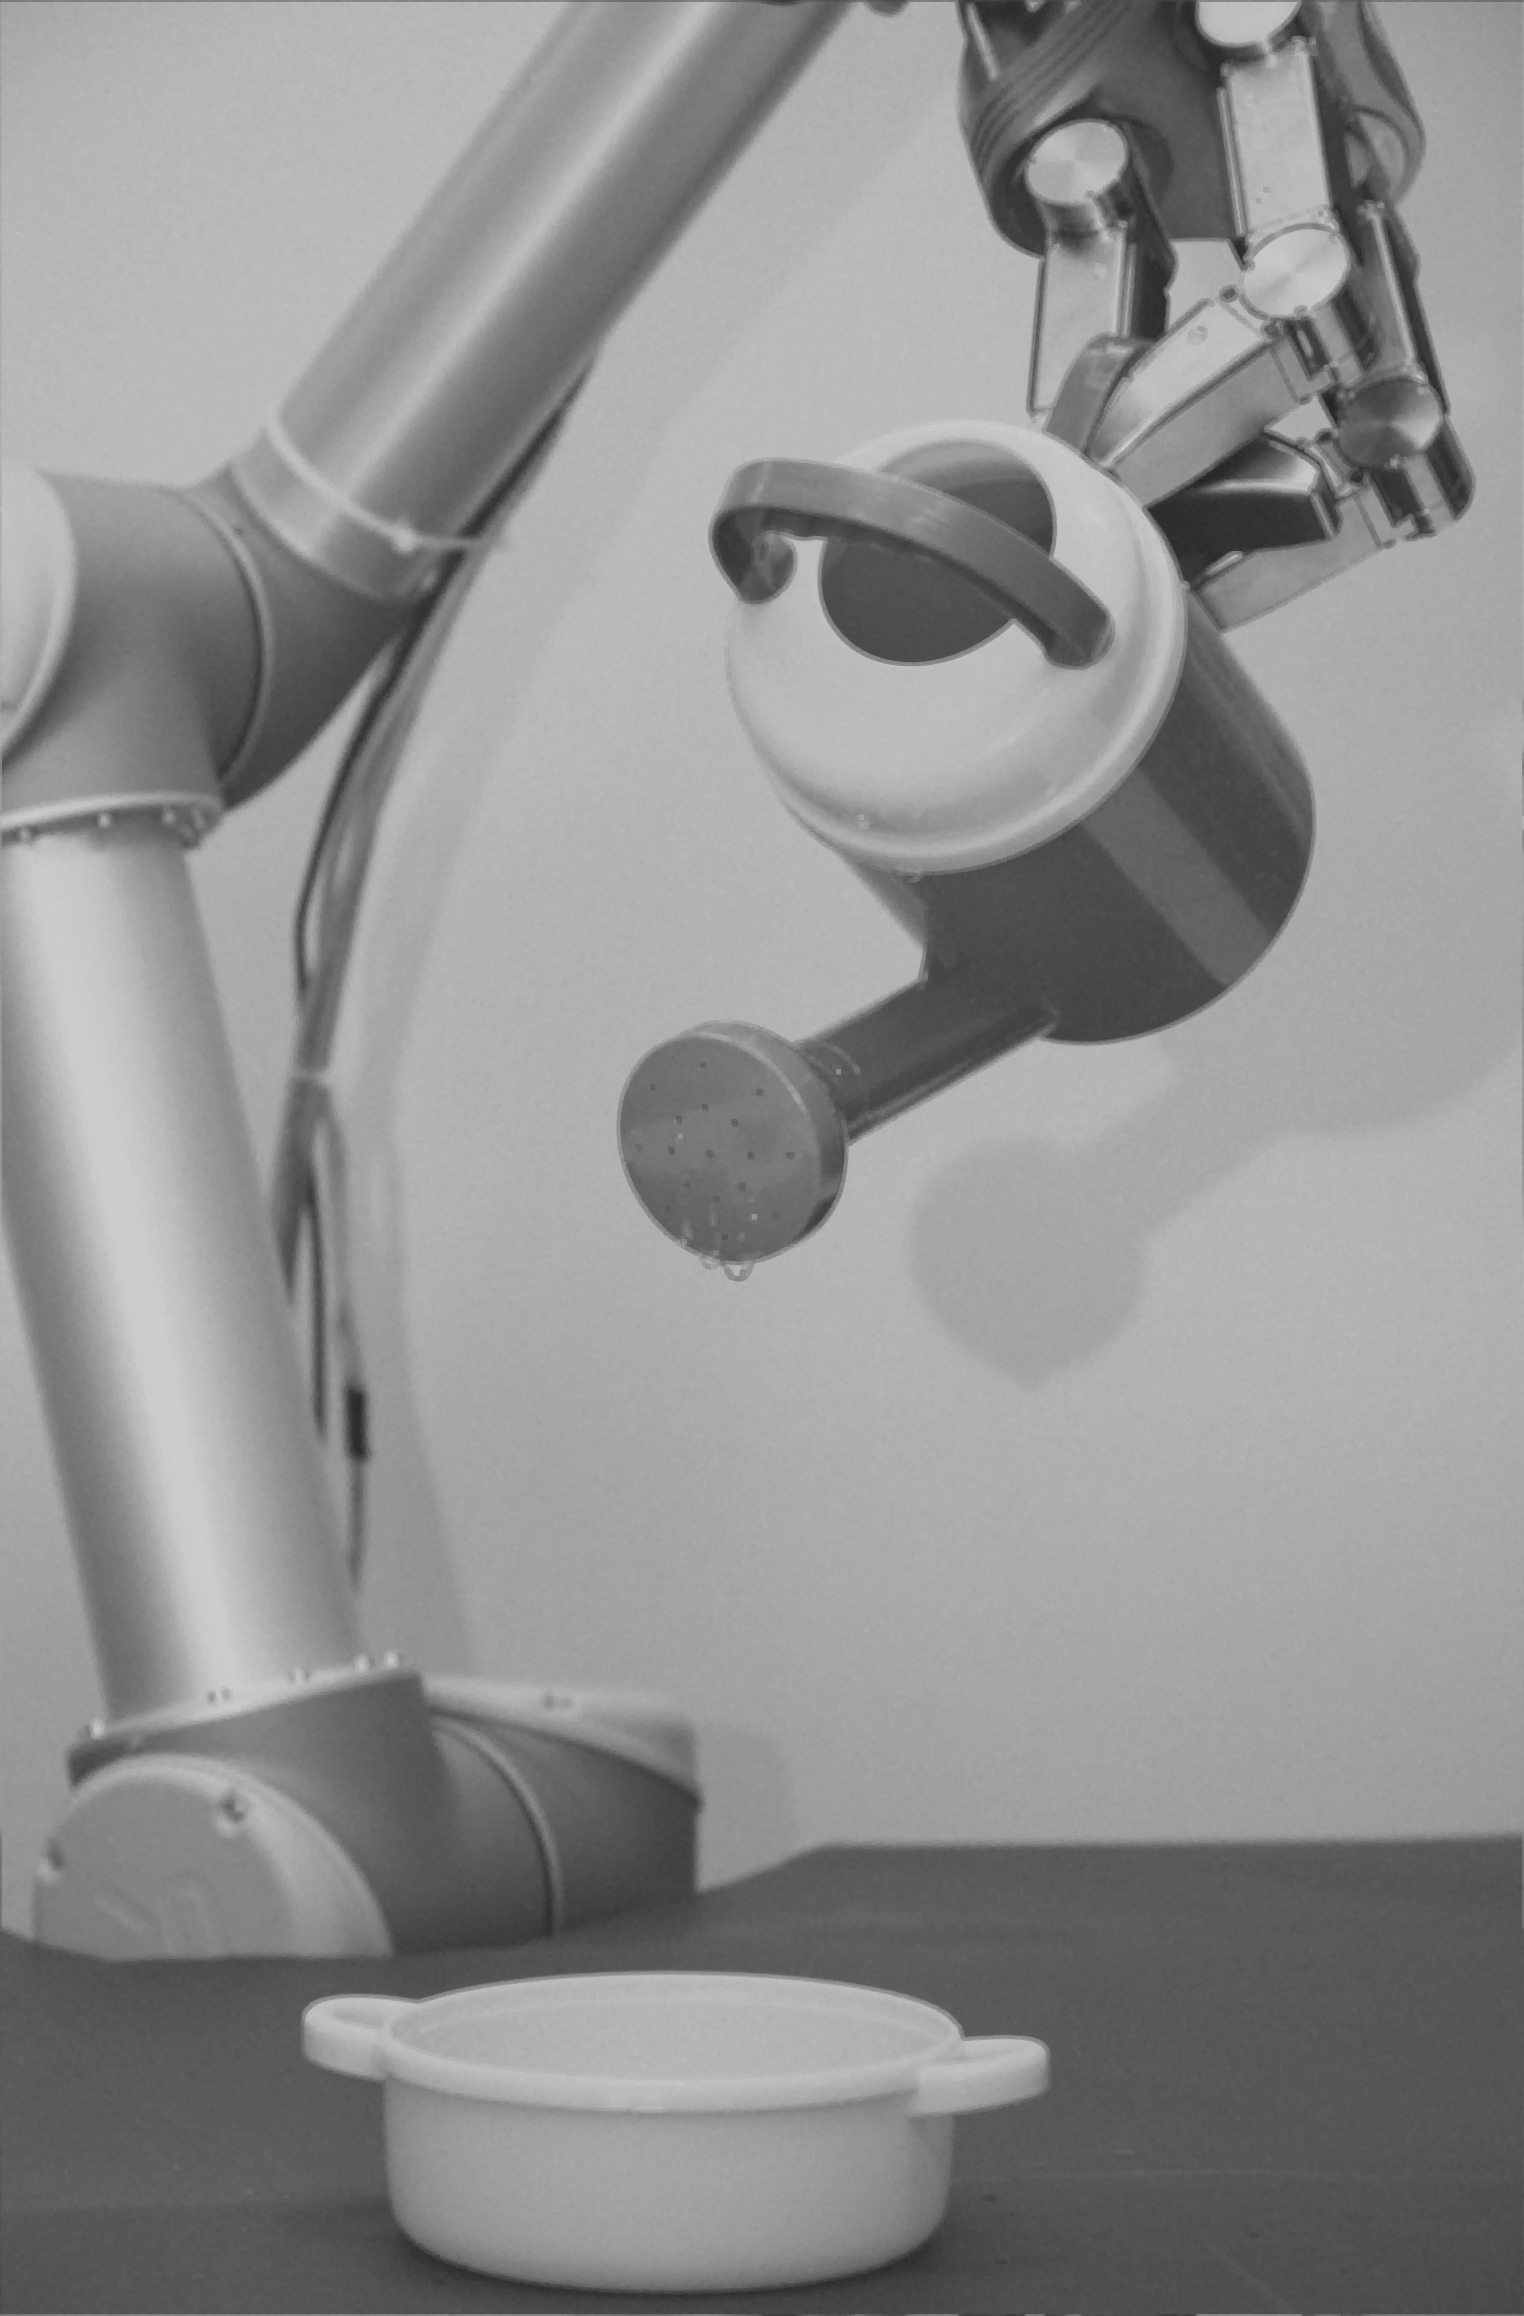
\includegraphics[width=\textwidth]{img3/test/contrast_5_0_8_final_img3.png}
    \end{subfigure}
    \begin{subfigure}[b]{0.1\textwidth}
        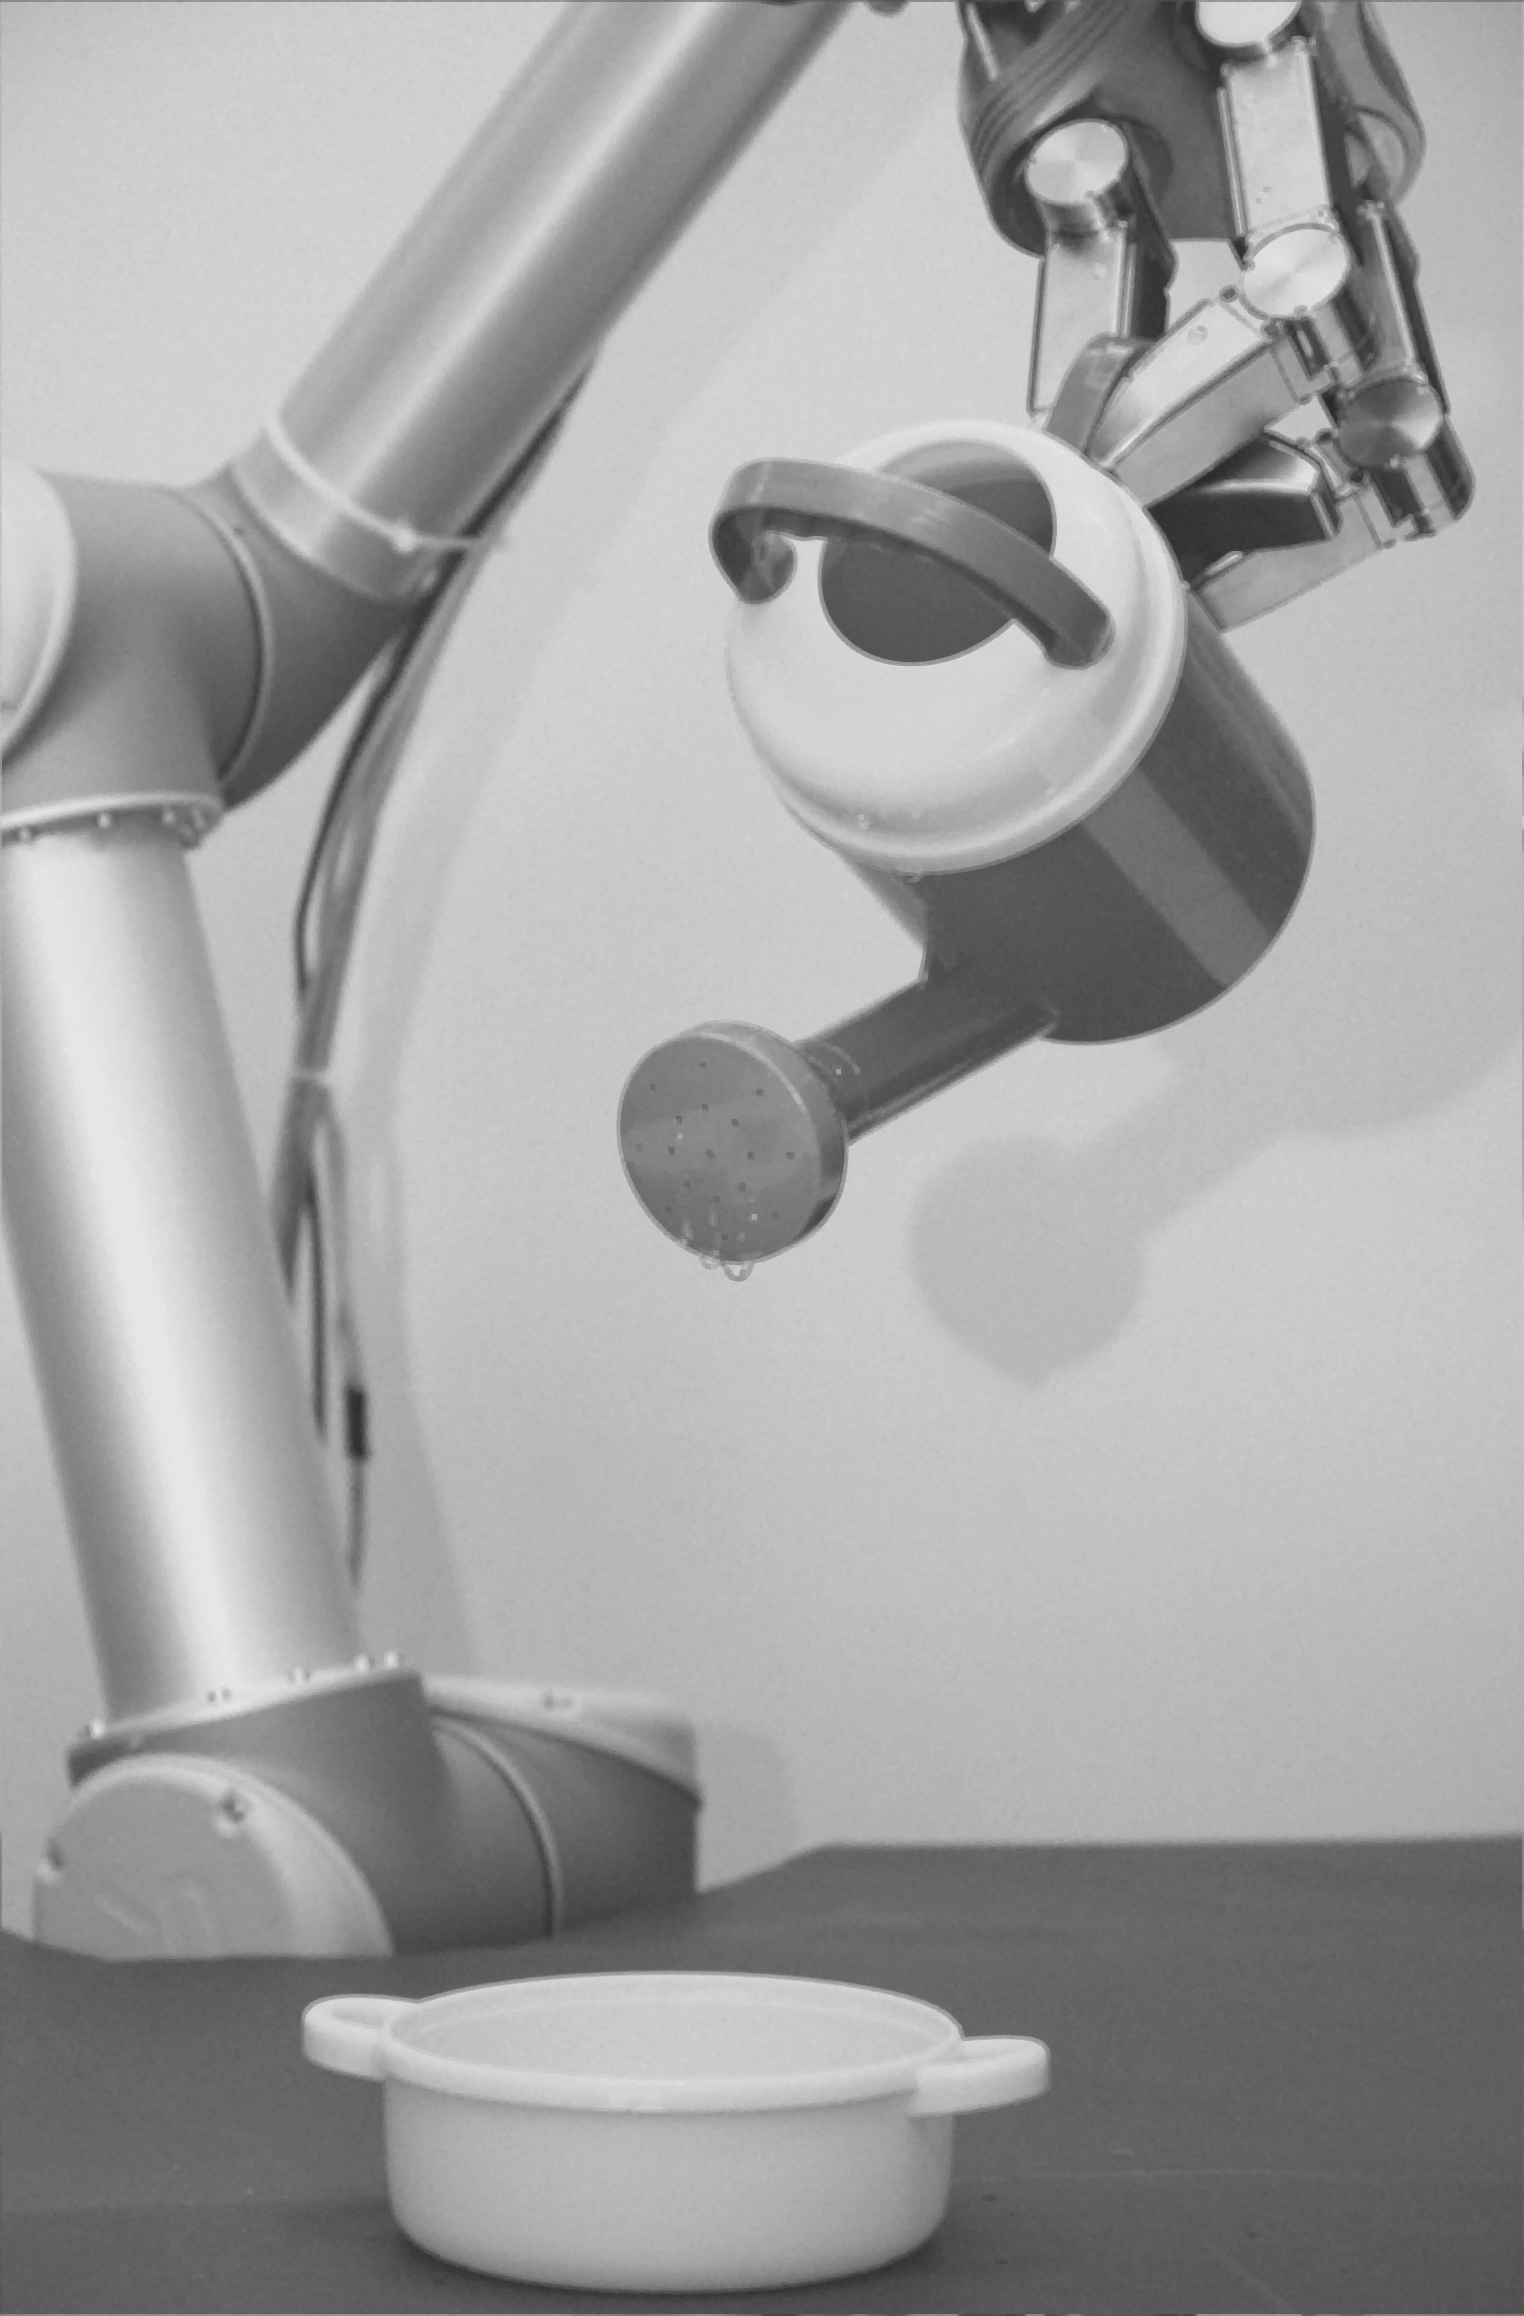
\includegraphics[width=\textwidth]{img3/test/contrast_5_0_9_final_img3.png}
    \end{subfigure}
    \begin{subfigure}[b]{0.1\textwidth}
        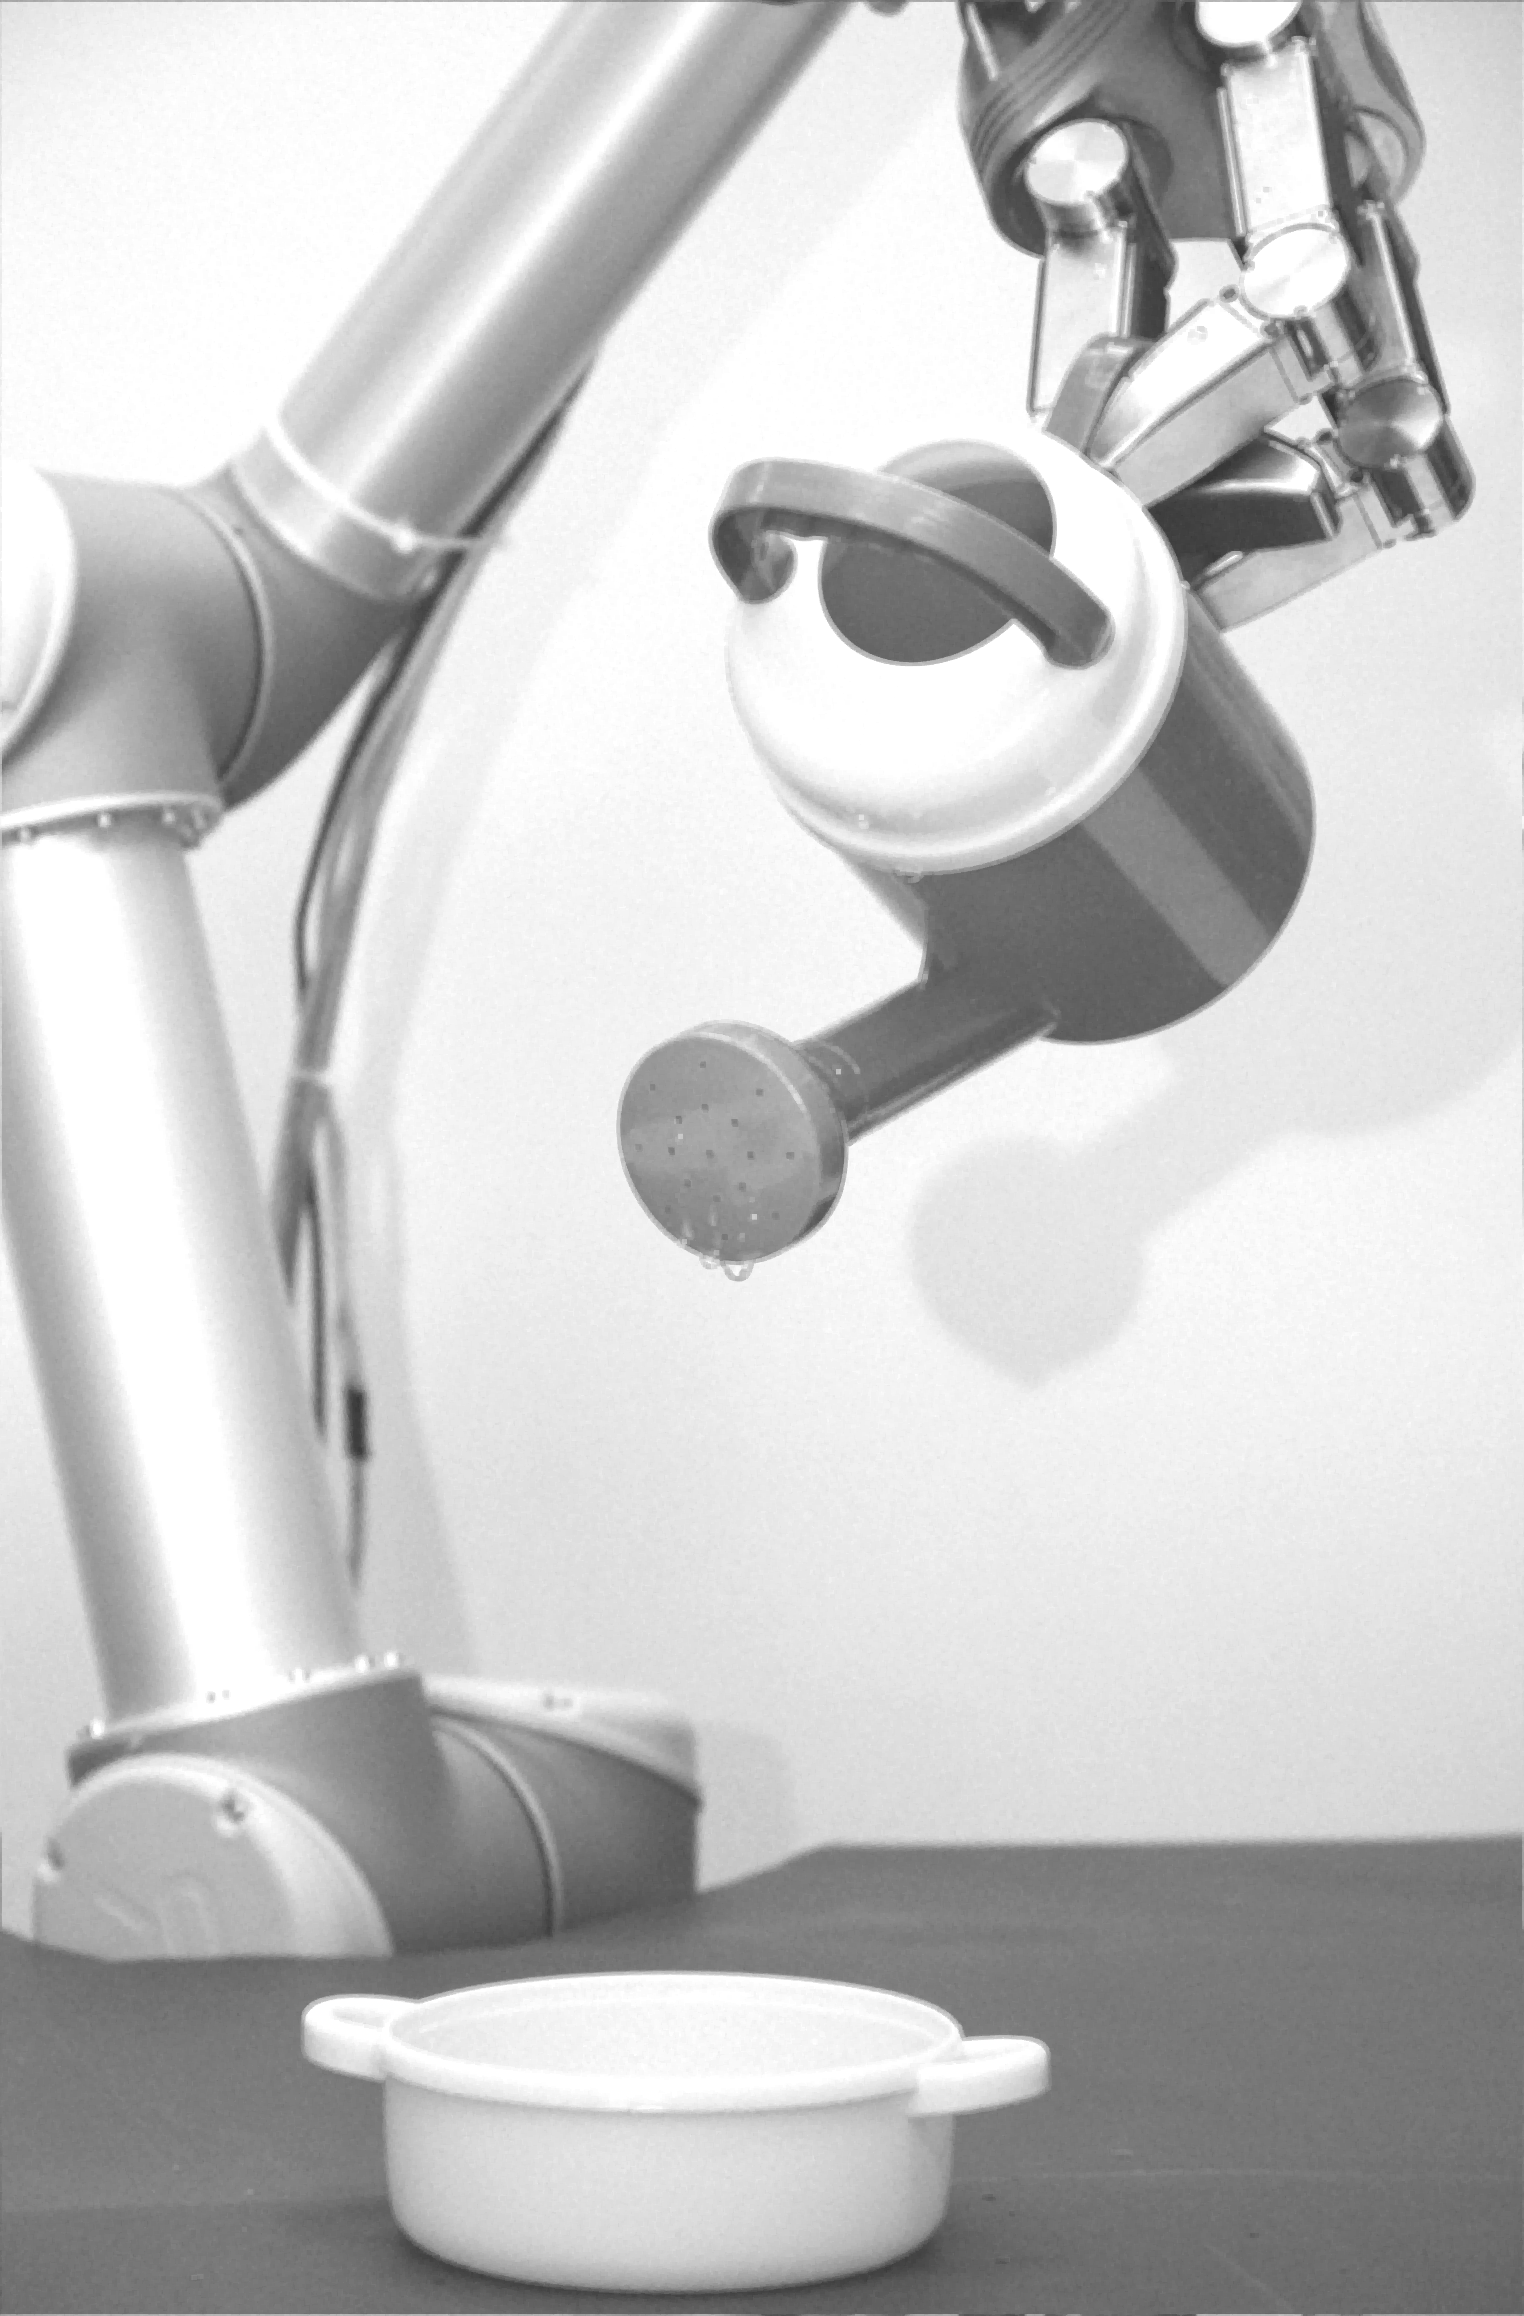
\includegraphics[width=\textwidth]{img3/test/contrast_5_1_1_final_img3.png}
    \end{subfigure}
        \begin{subfigure}[b]{0.1\textwidth}
        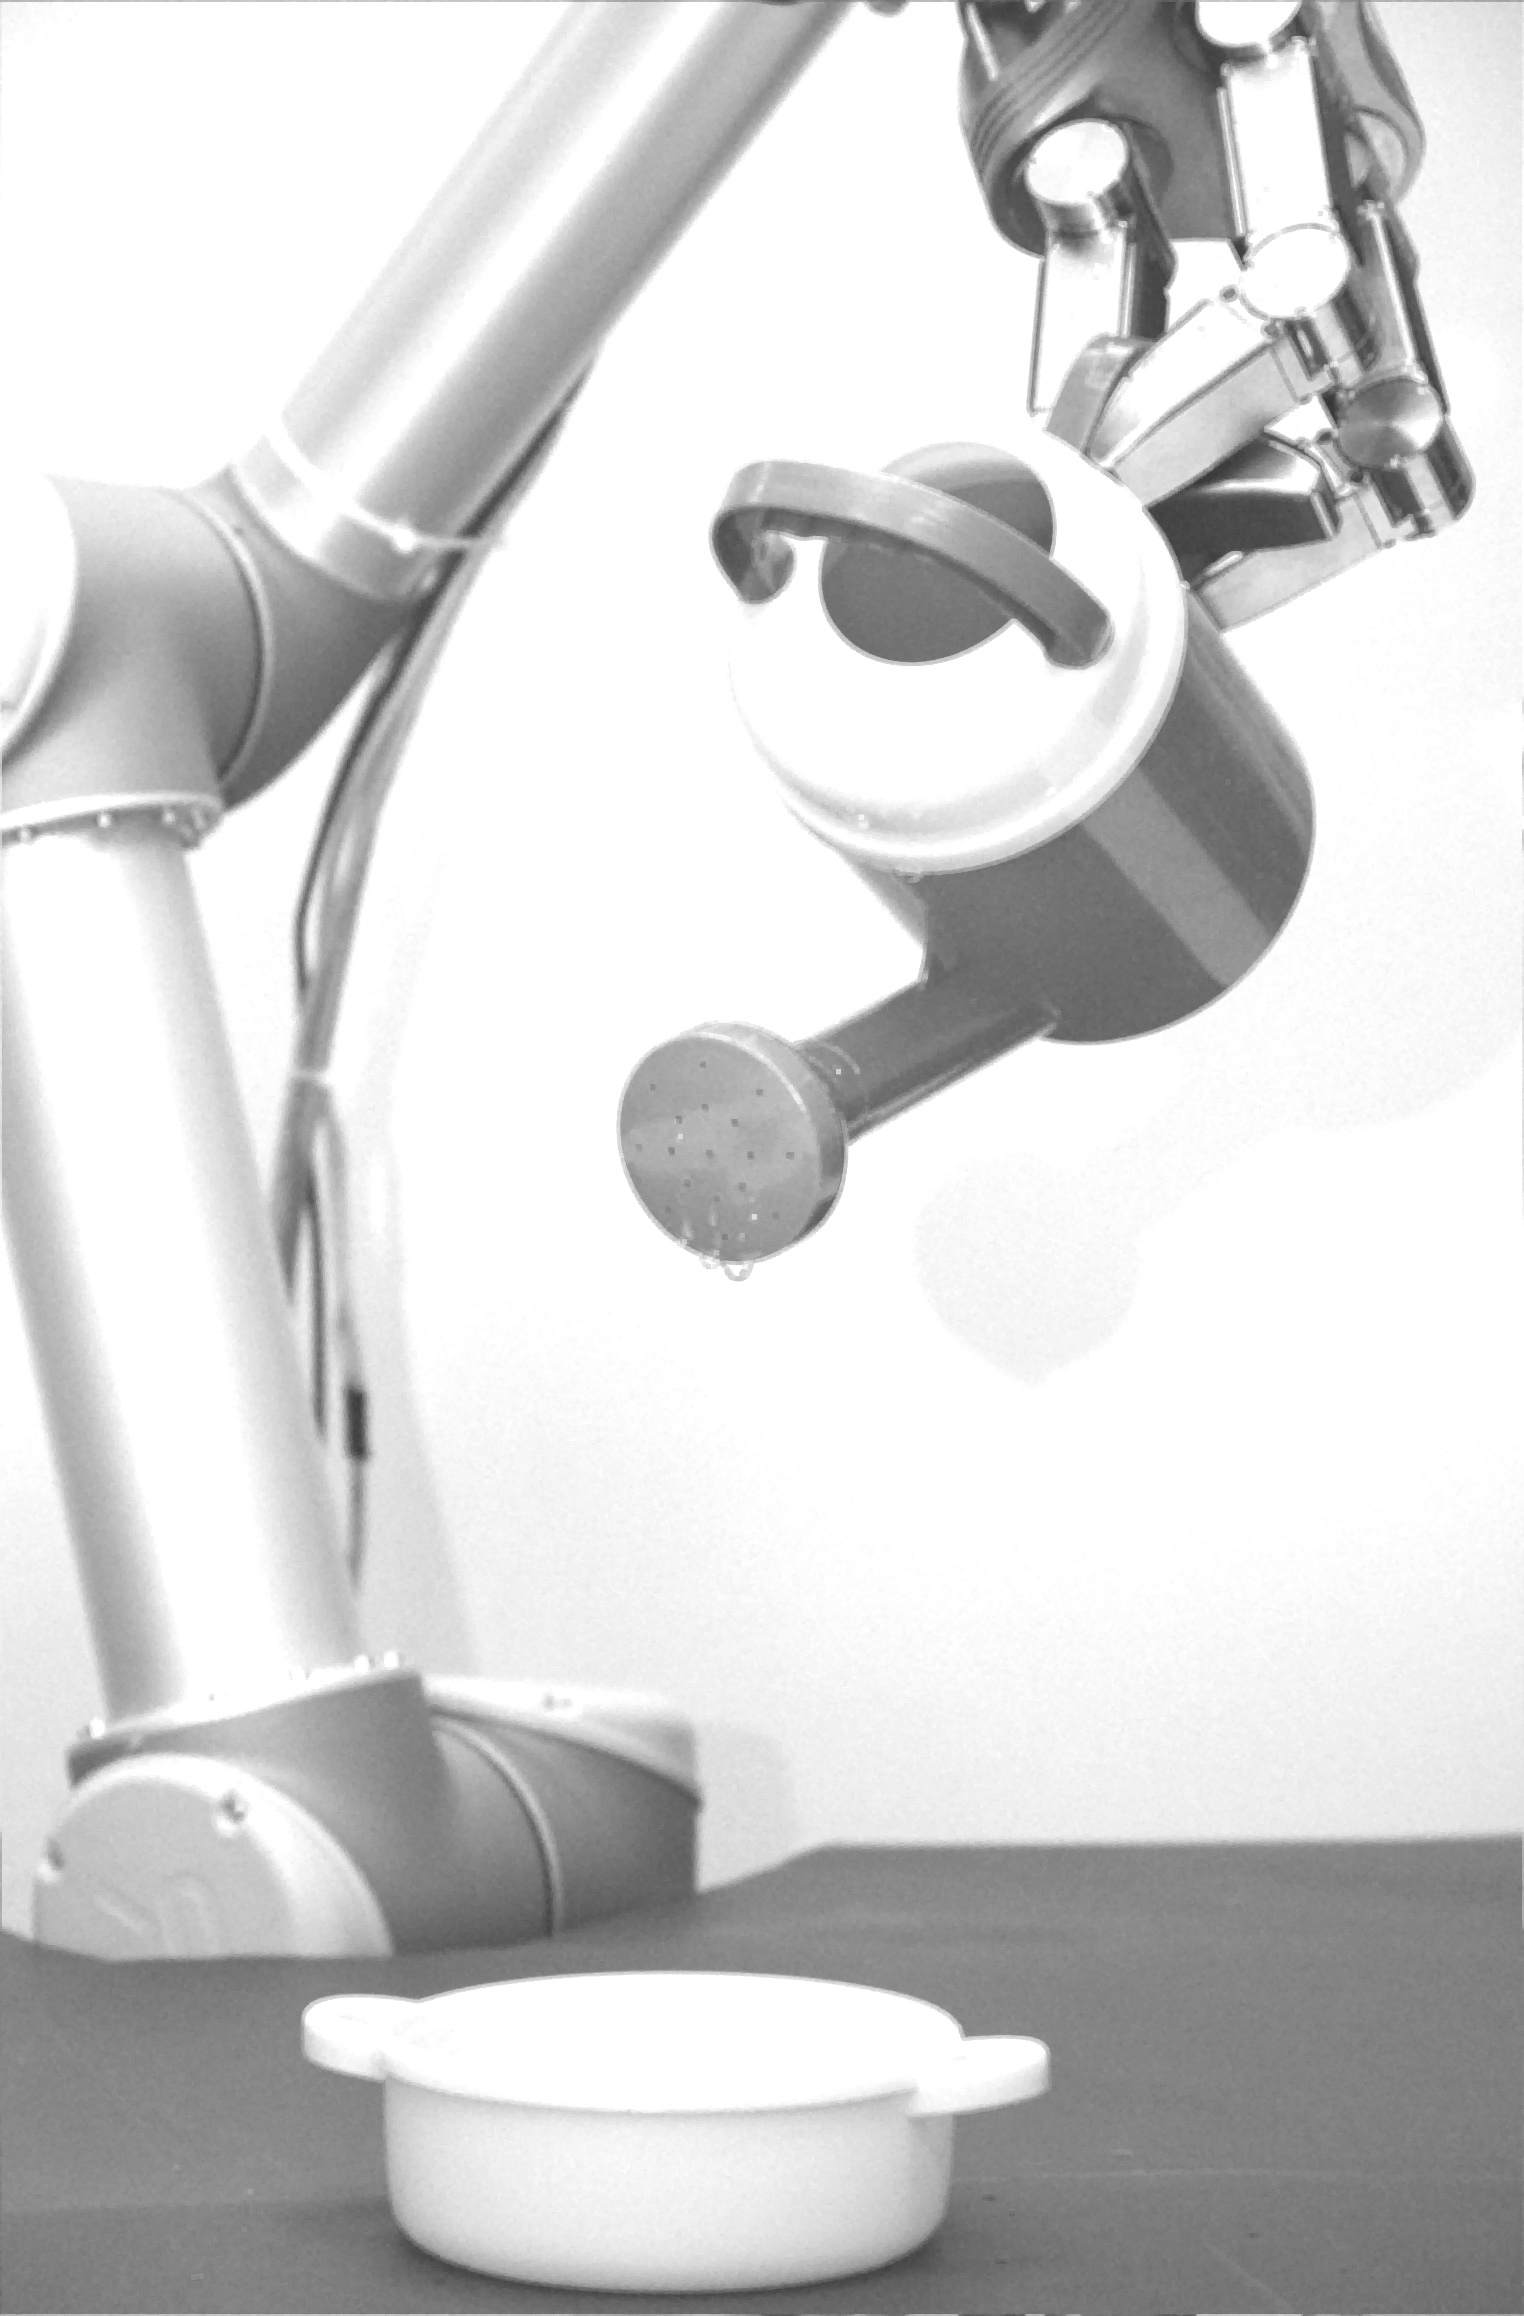
\includegraphics[width=\textwidth]{img3/test/contrast_5_1_2_final_img3.png}
    \end{subfigure}
        \begin{subfigure}[b]{0.1\textwidth}
        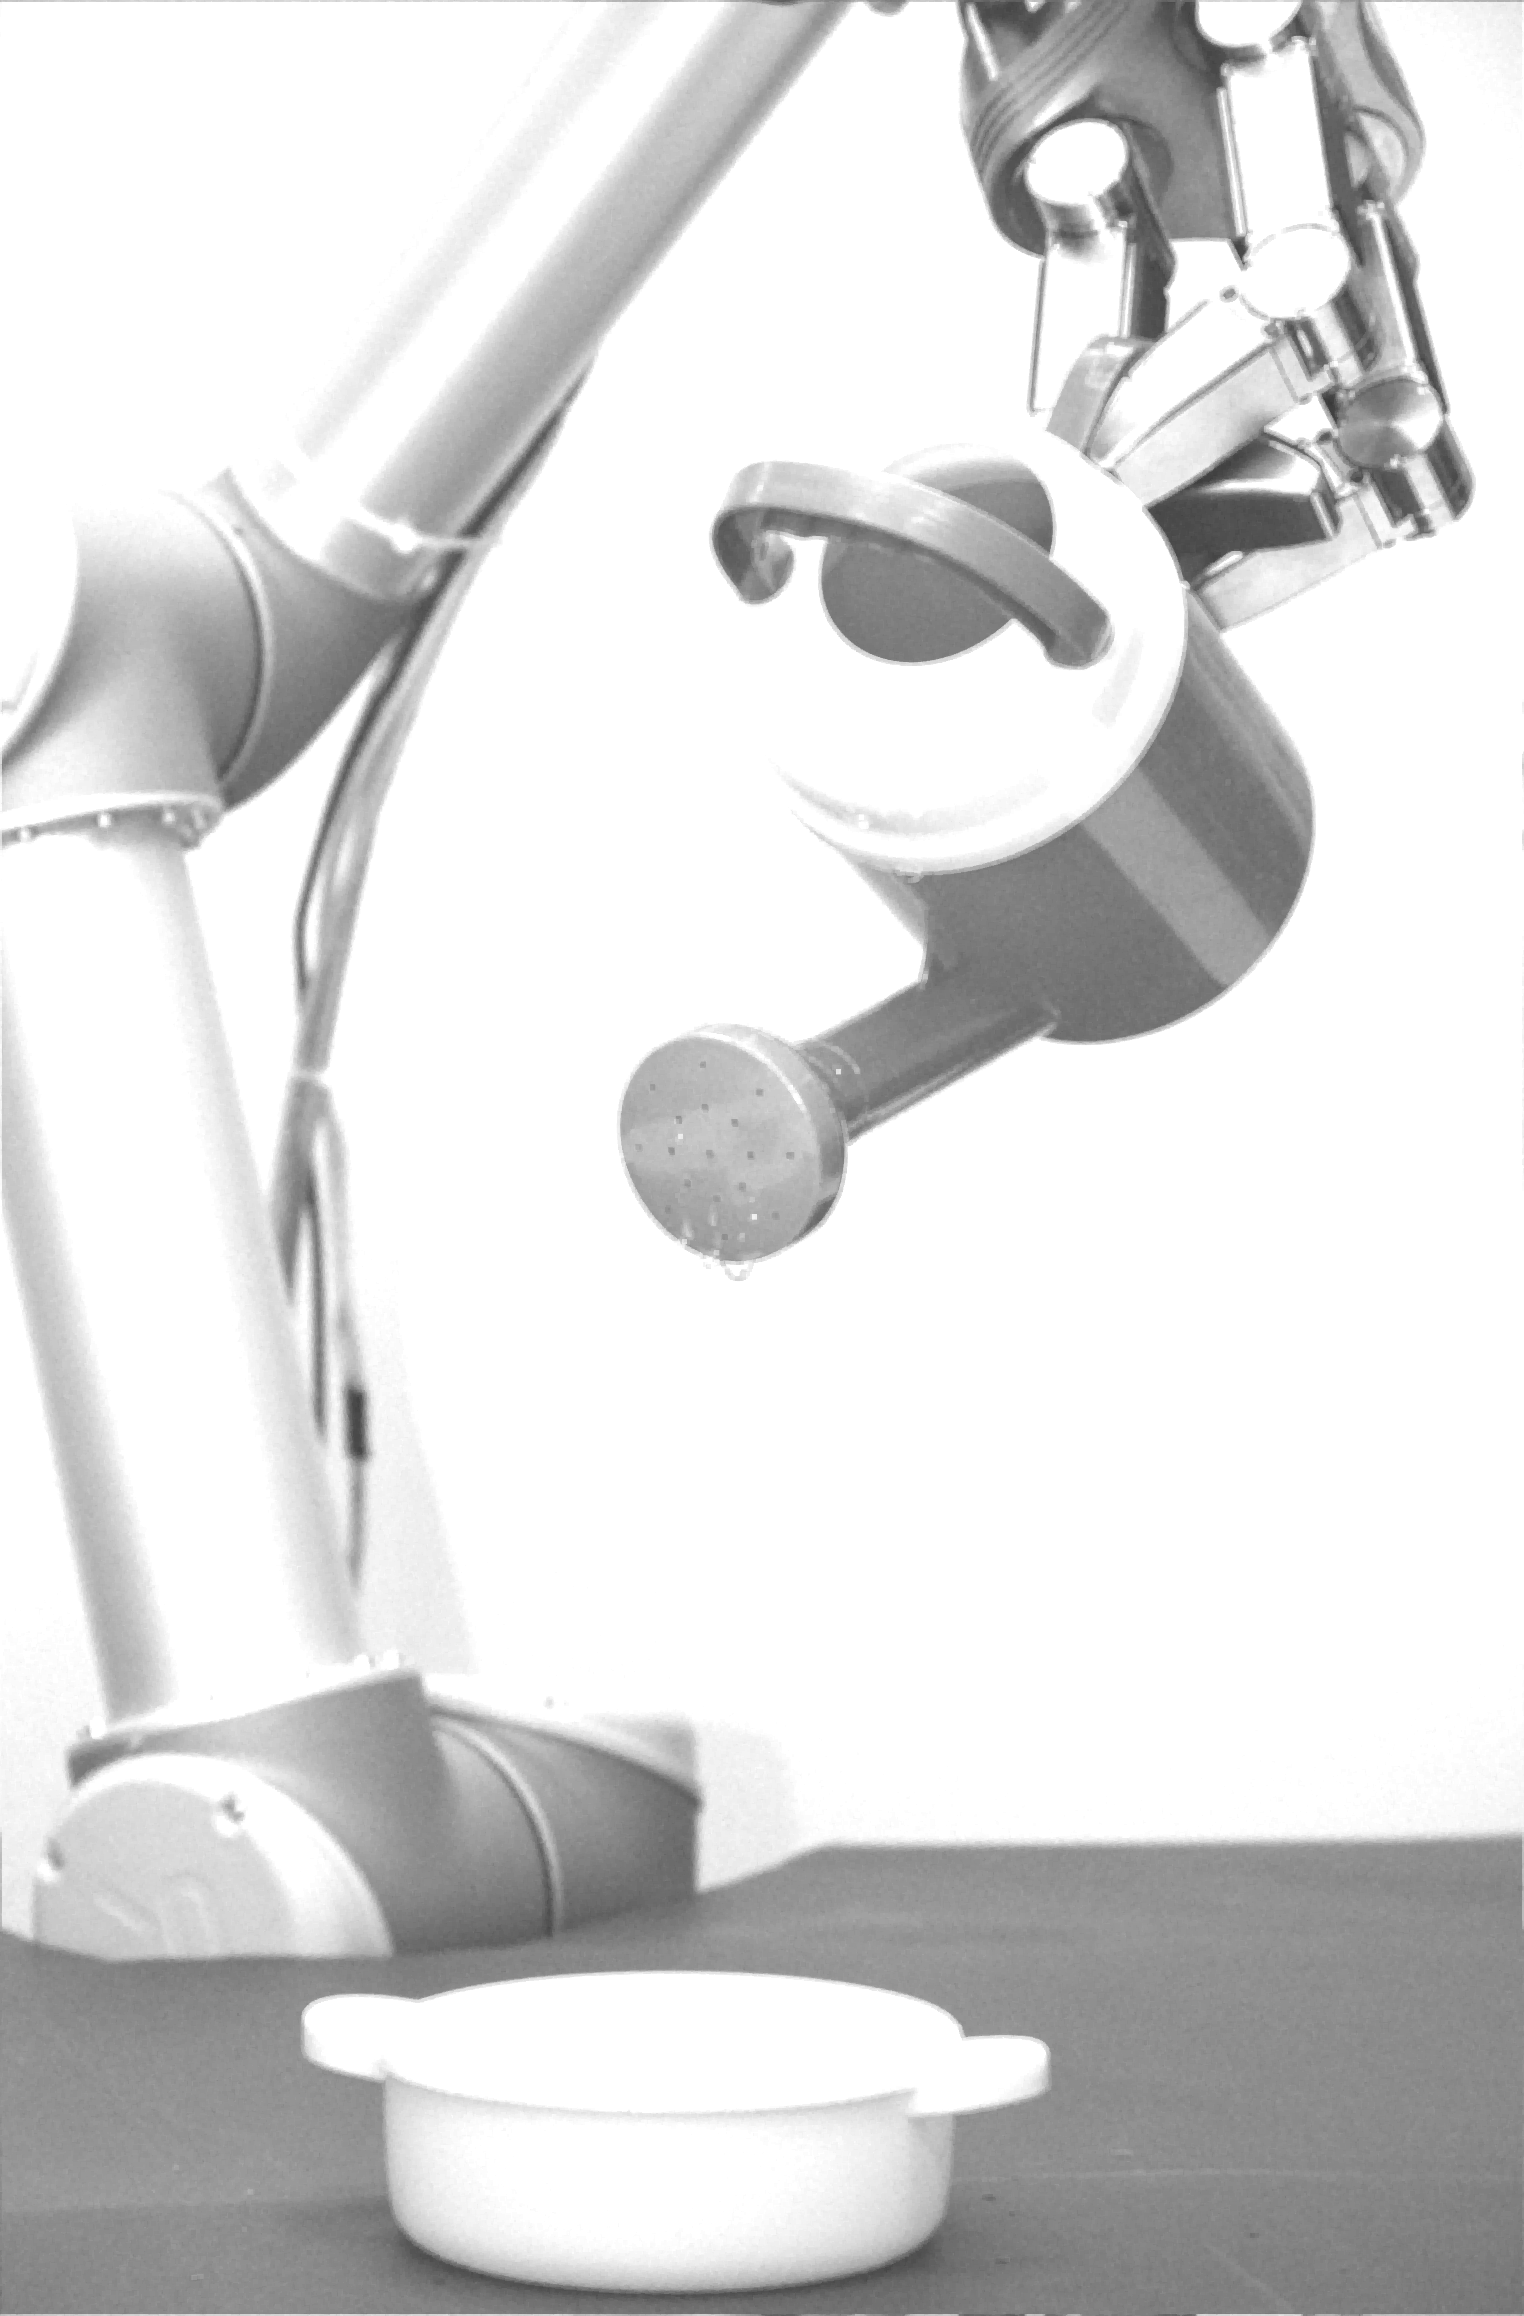
\includegraphics[width=\textwidth]{img3/test/contrast_5_1_3_final_img3.png}
    \end{subfigure}
        \begin{subfigure}[b]{0.1\textwidth}
        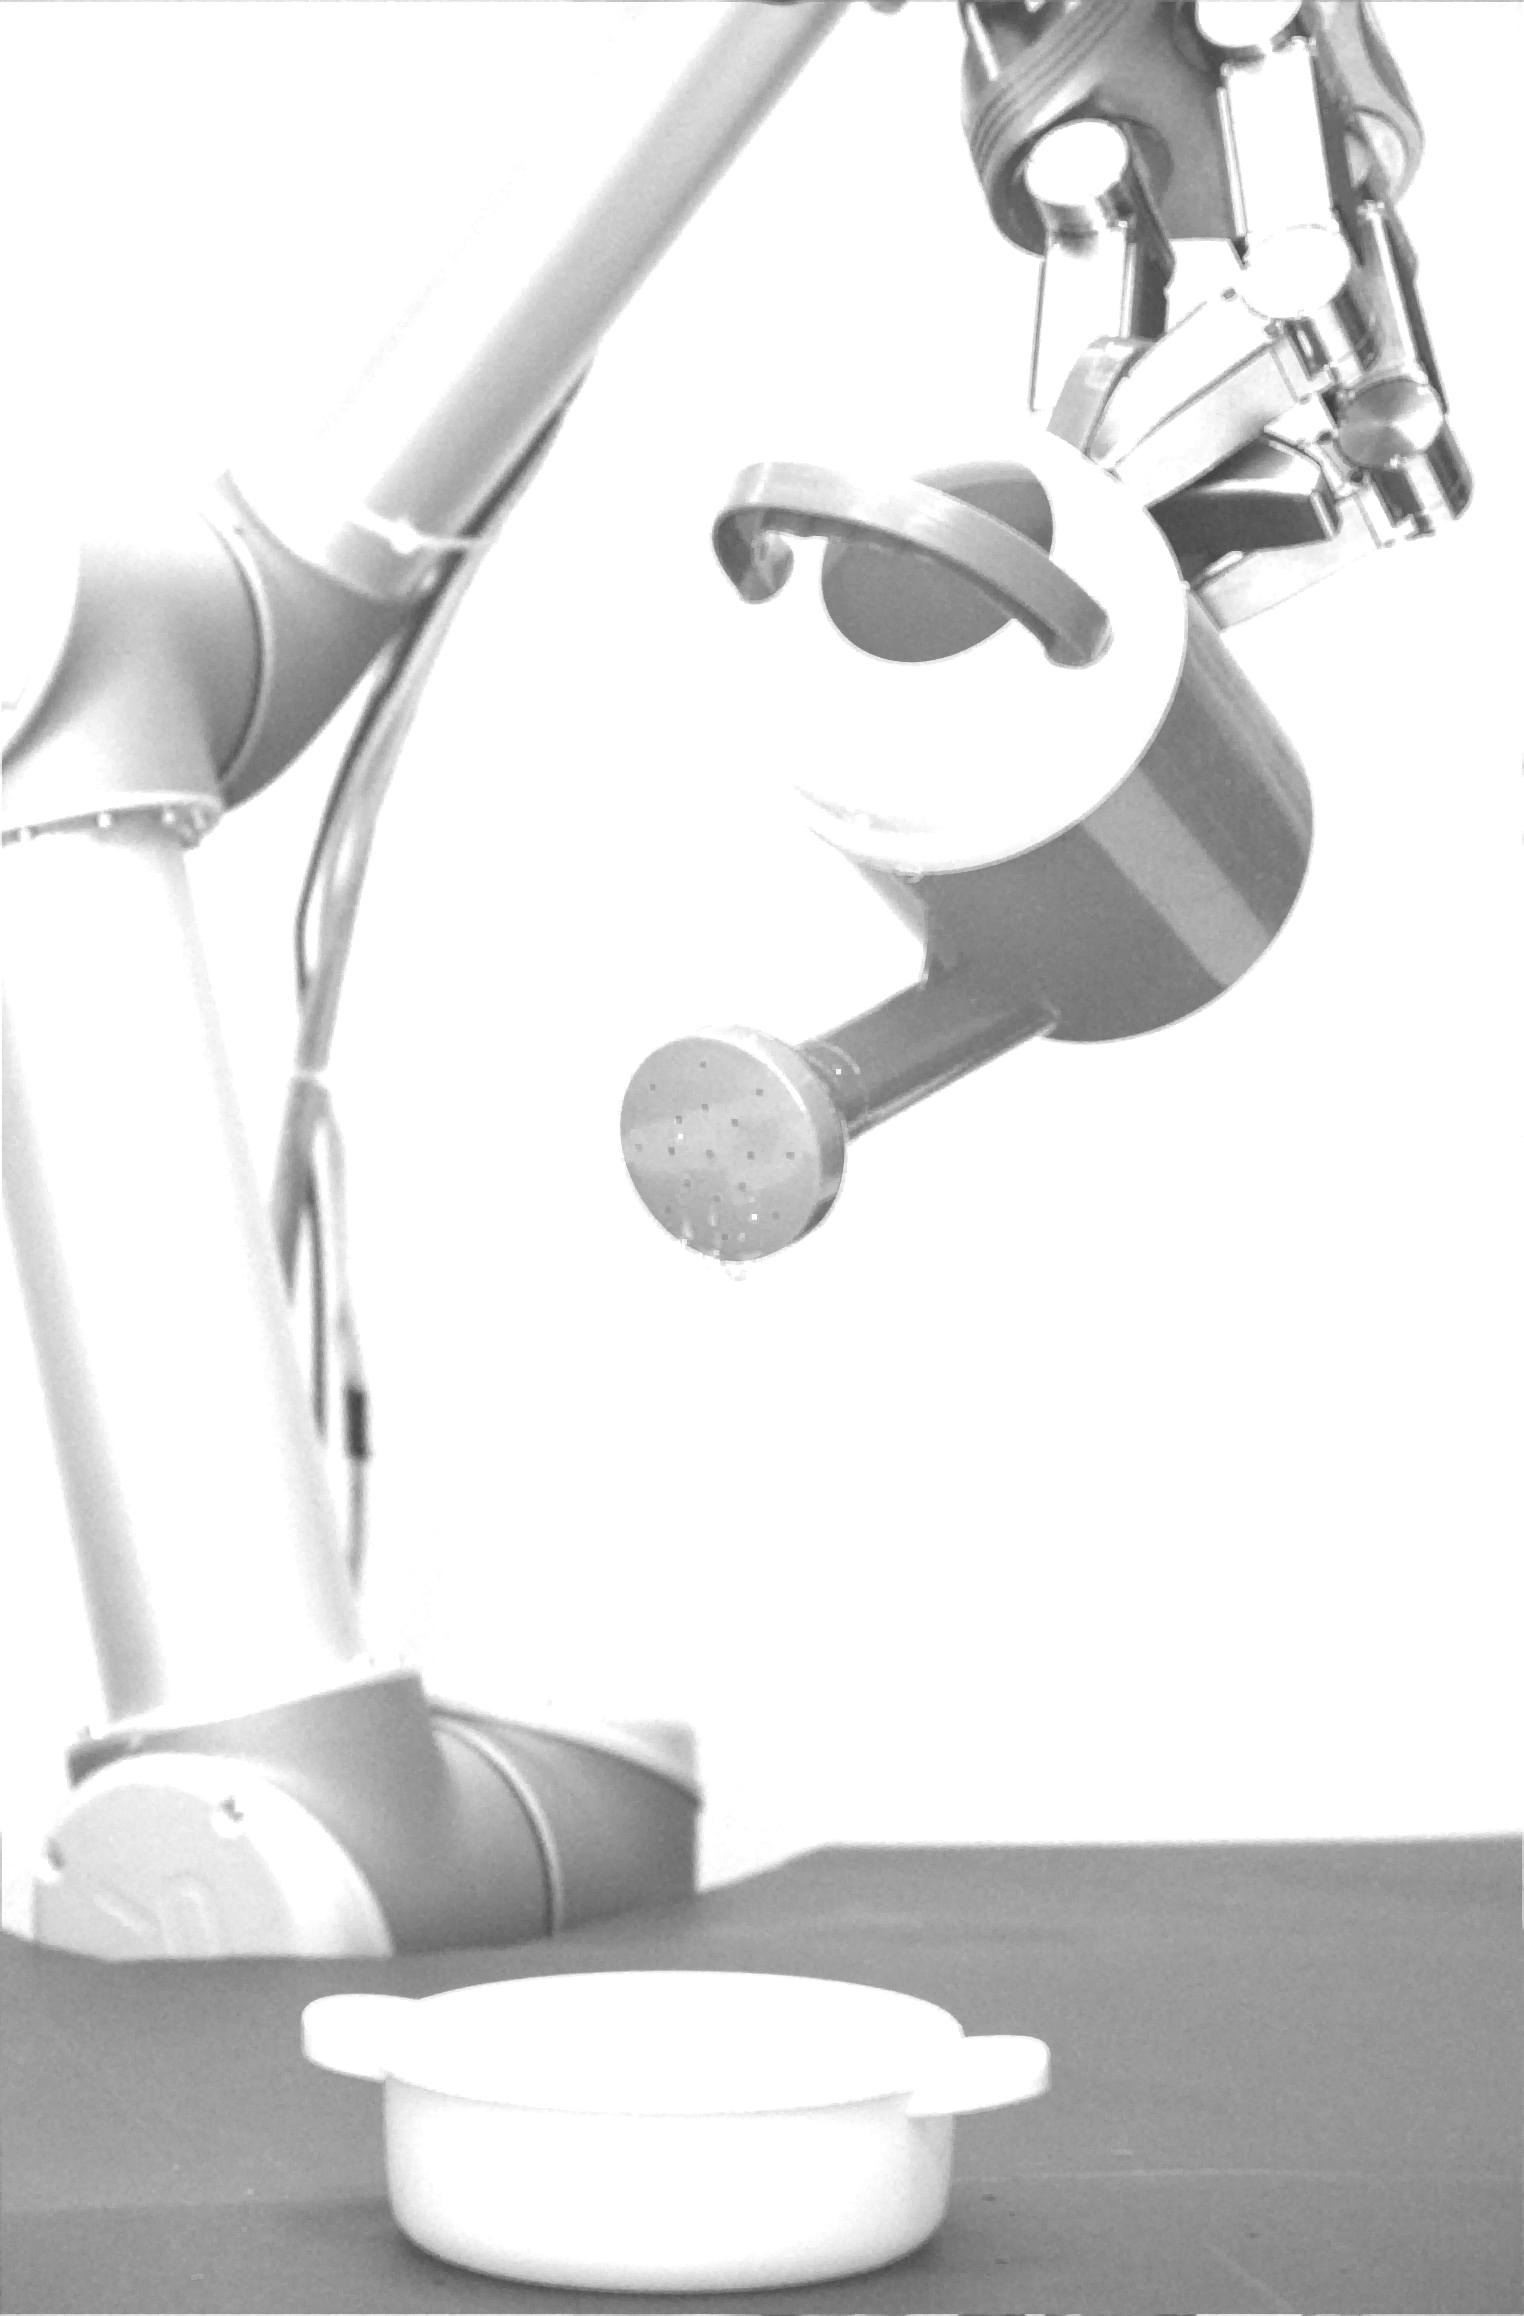
\includegraphics[width=\textwidth]{img3/test/contrast_5_1_4_final_img3.png}
    \end{subfigure}
        \begin{subfigure}[b]{0.1\textwidth}
        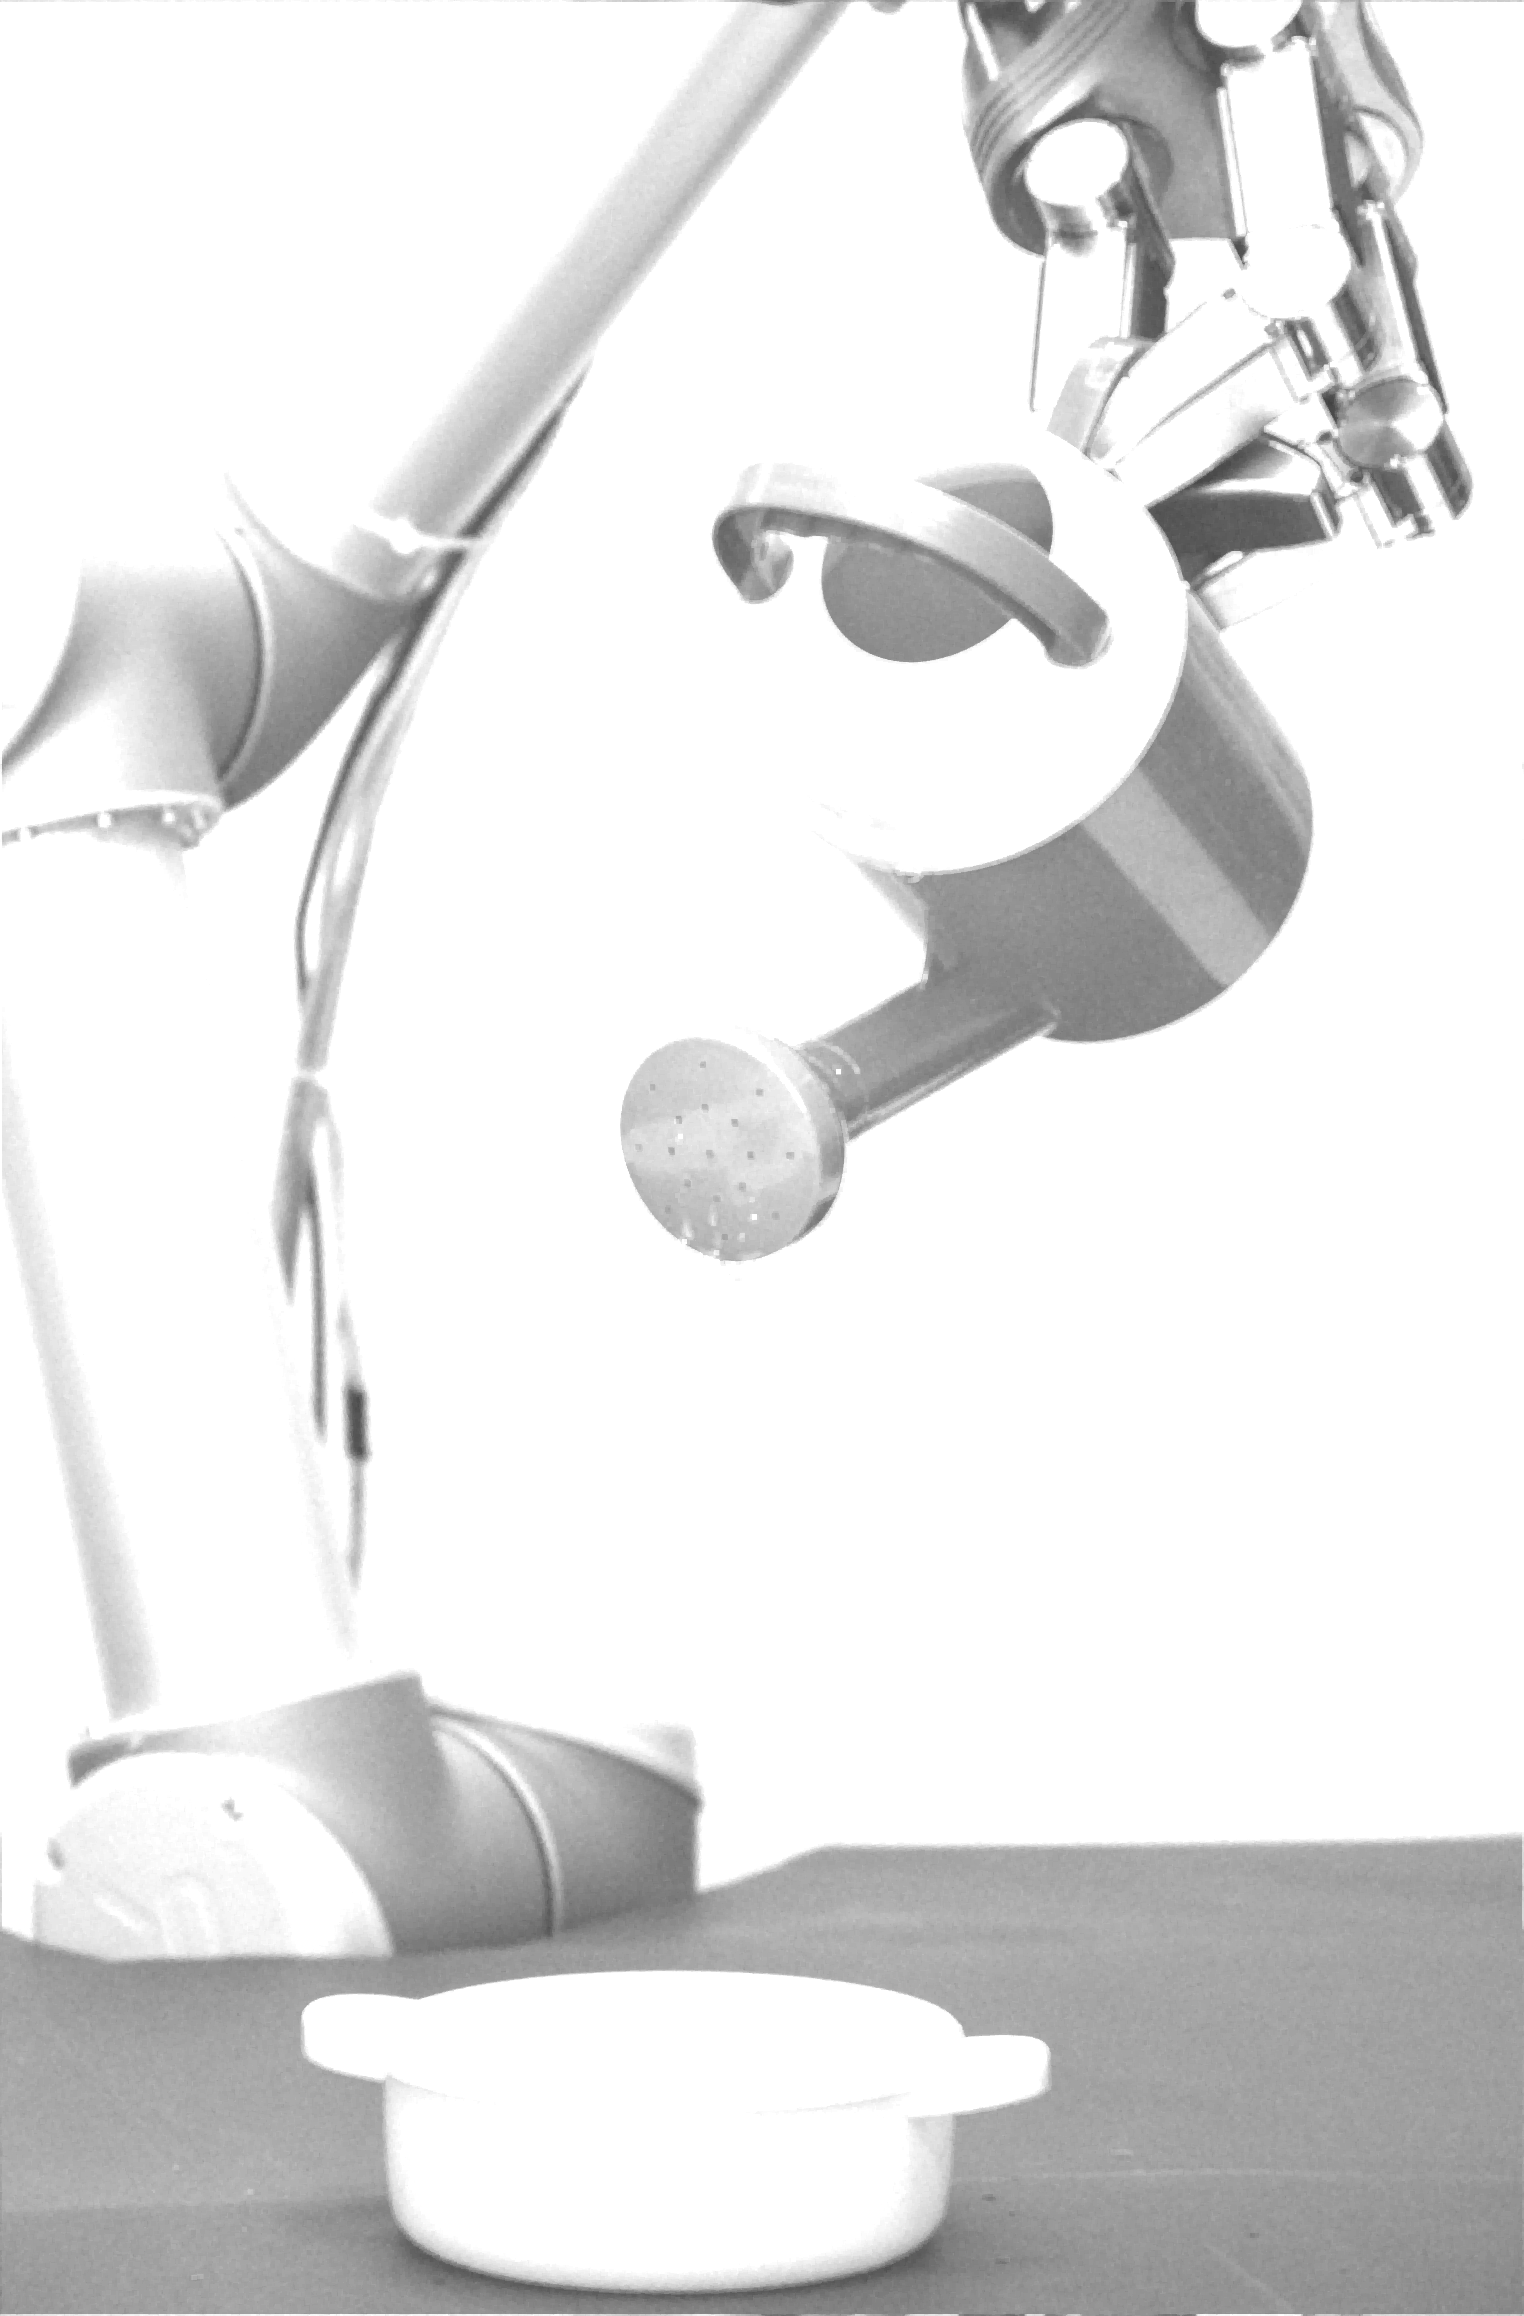
\includegraphics[width=\textwidth]{img3/test/contrast_5_1_5_final_img3.png}
    \end{subfigure}
        \begin{subfigure}[b]{0.1\textwidth}
        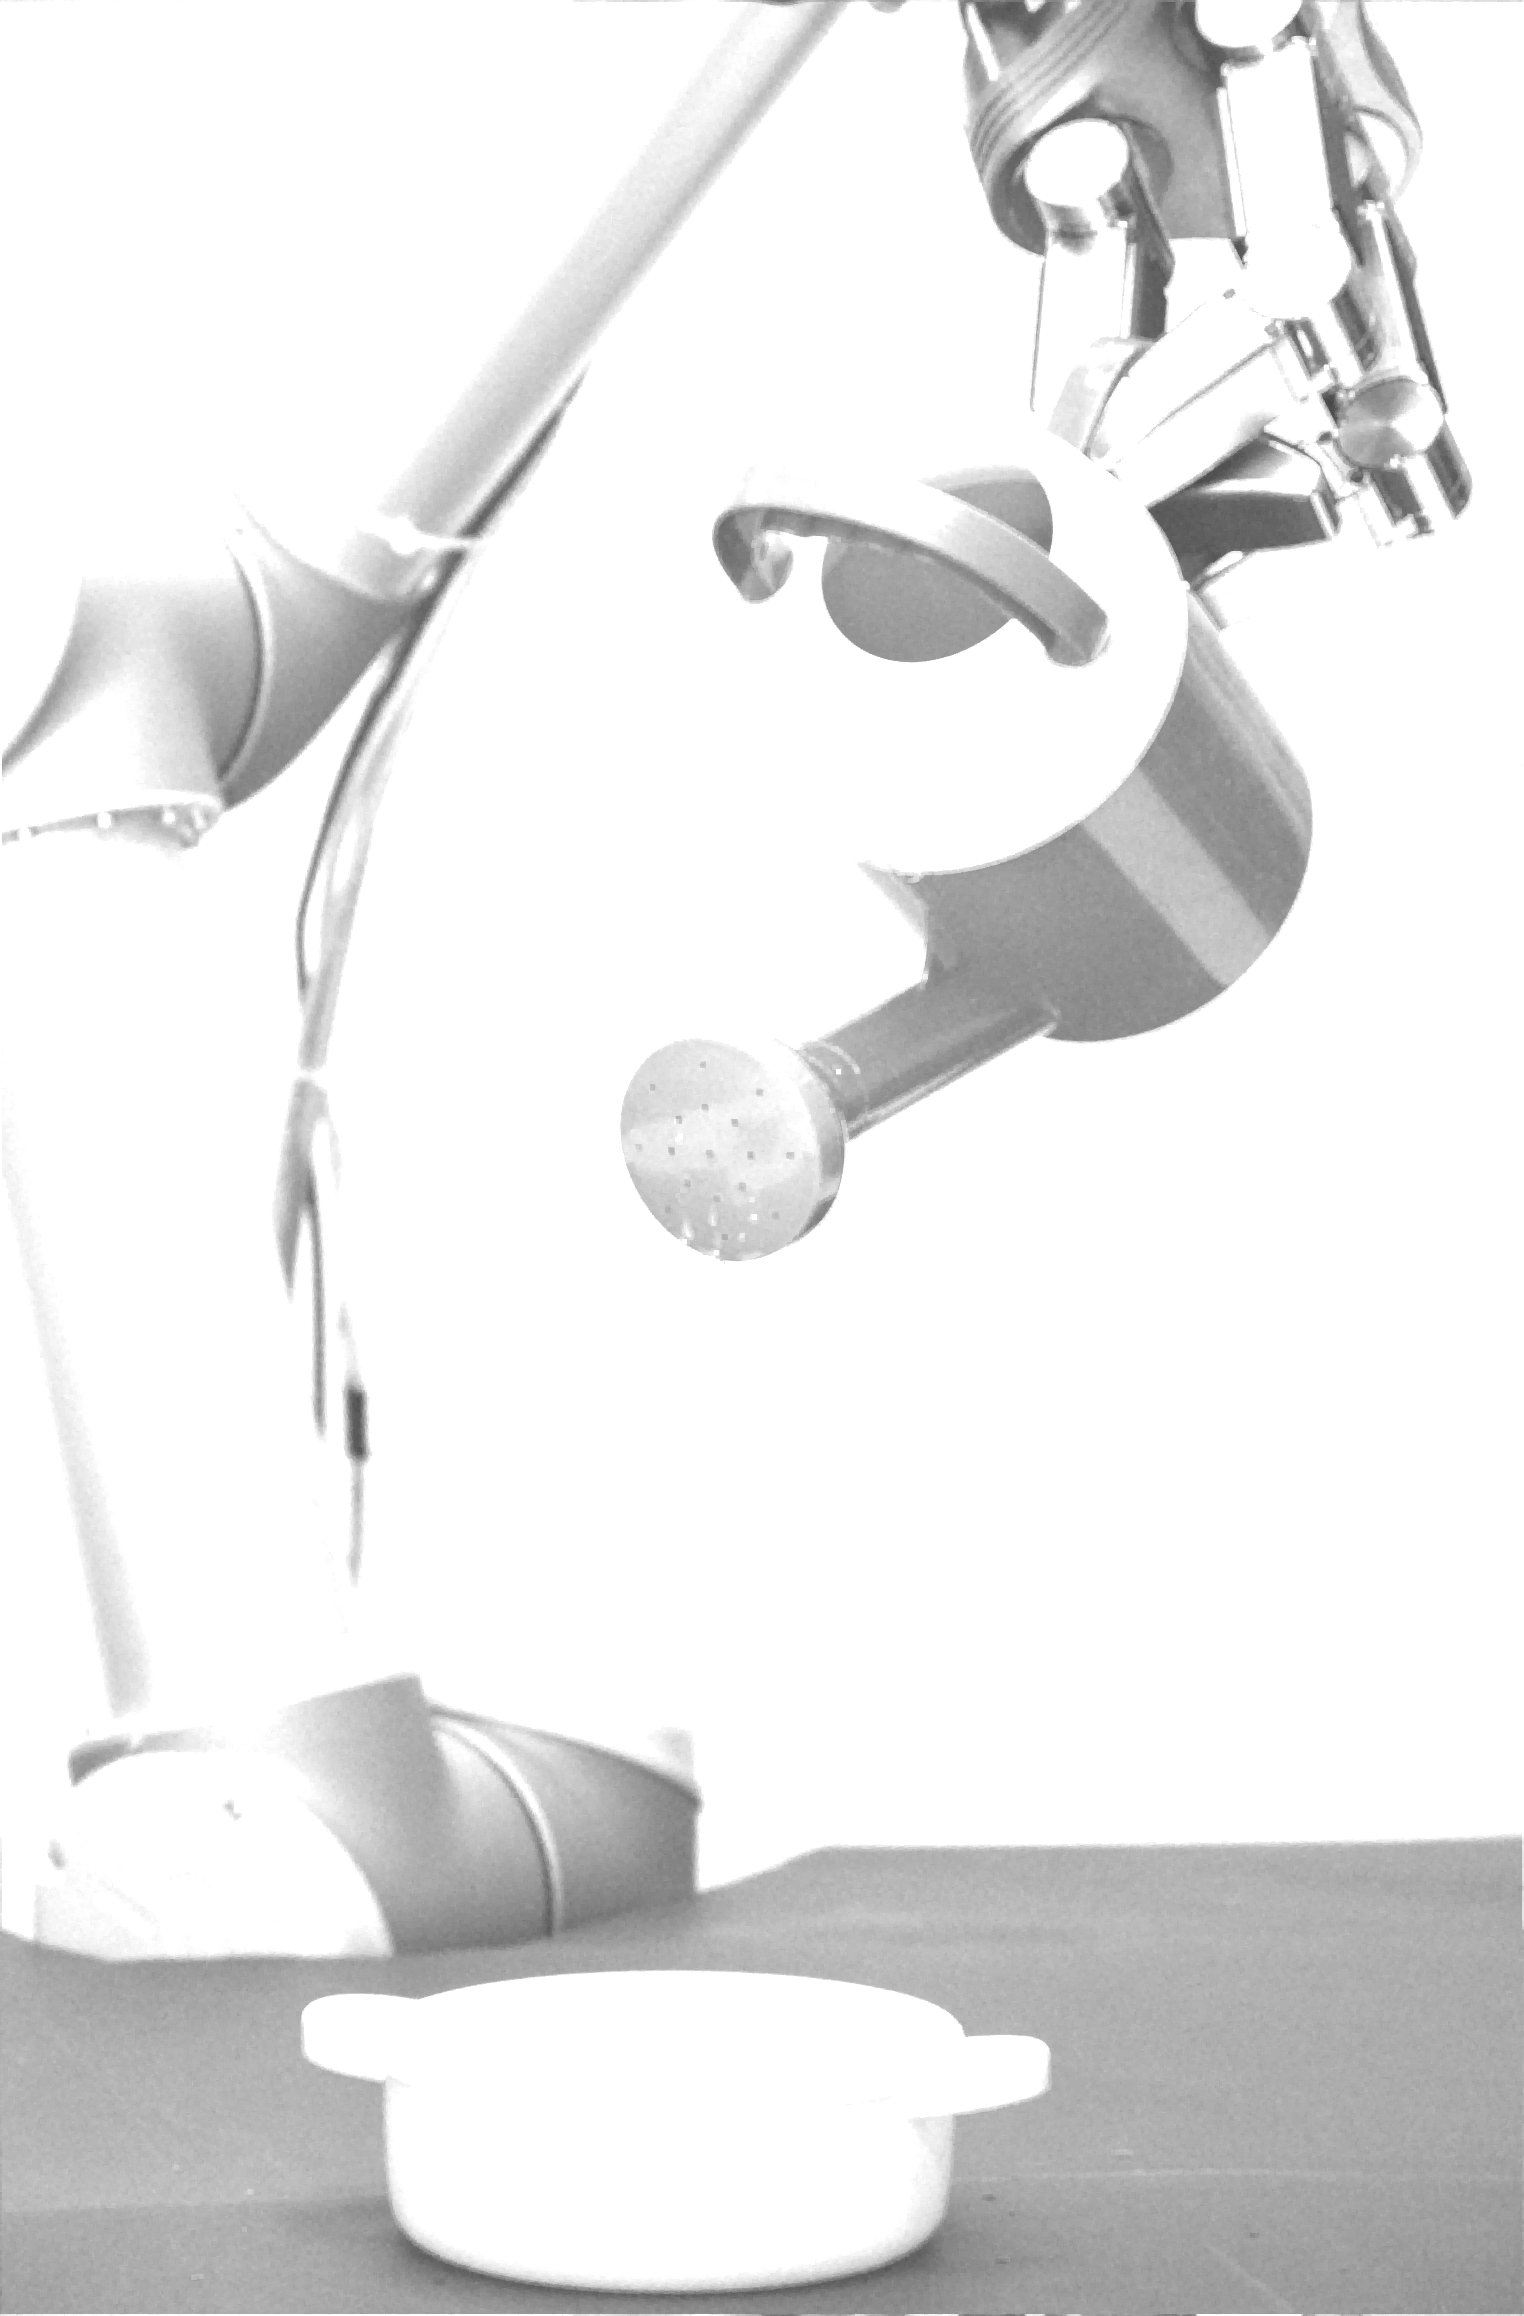
\includegraphics[width=\textwidth]{img3/test/contrast_5_1_6_final_img3.png}
    \end{subfigure}
        \begin{subfigure}[b]{0.1\textwidth}
        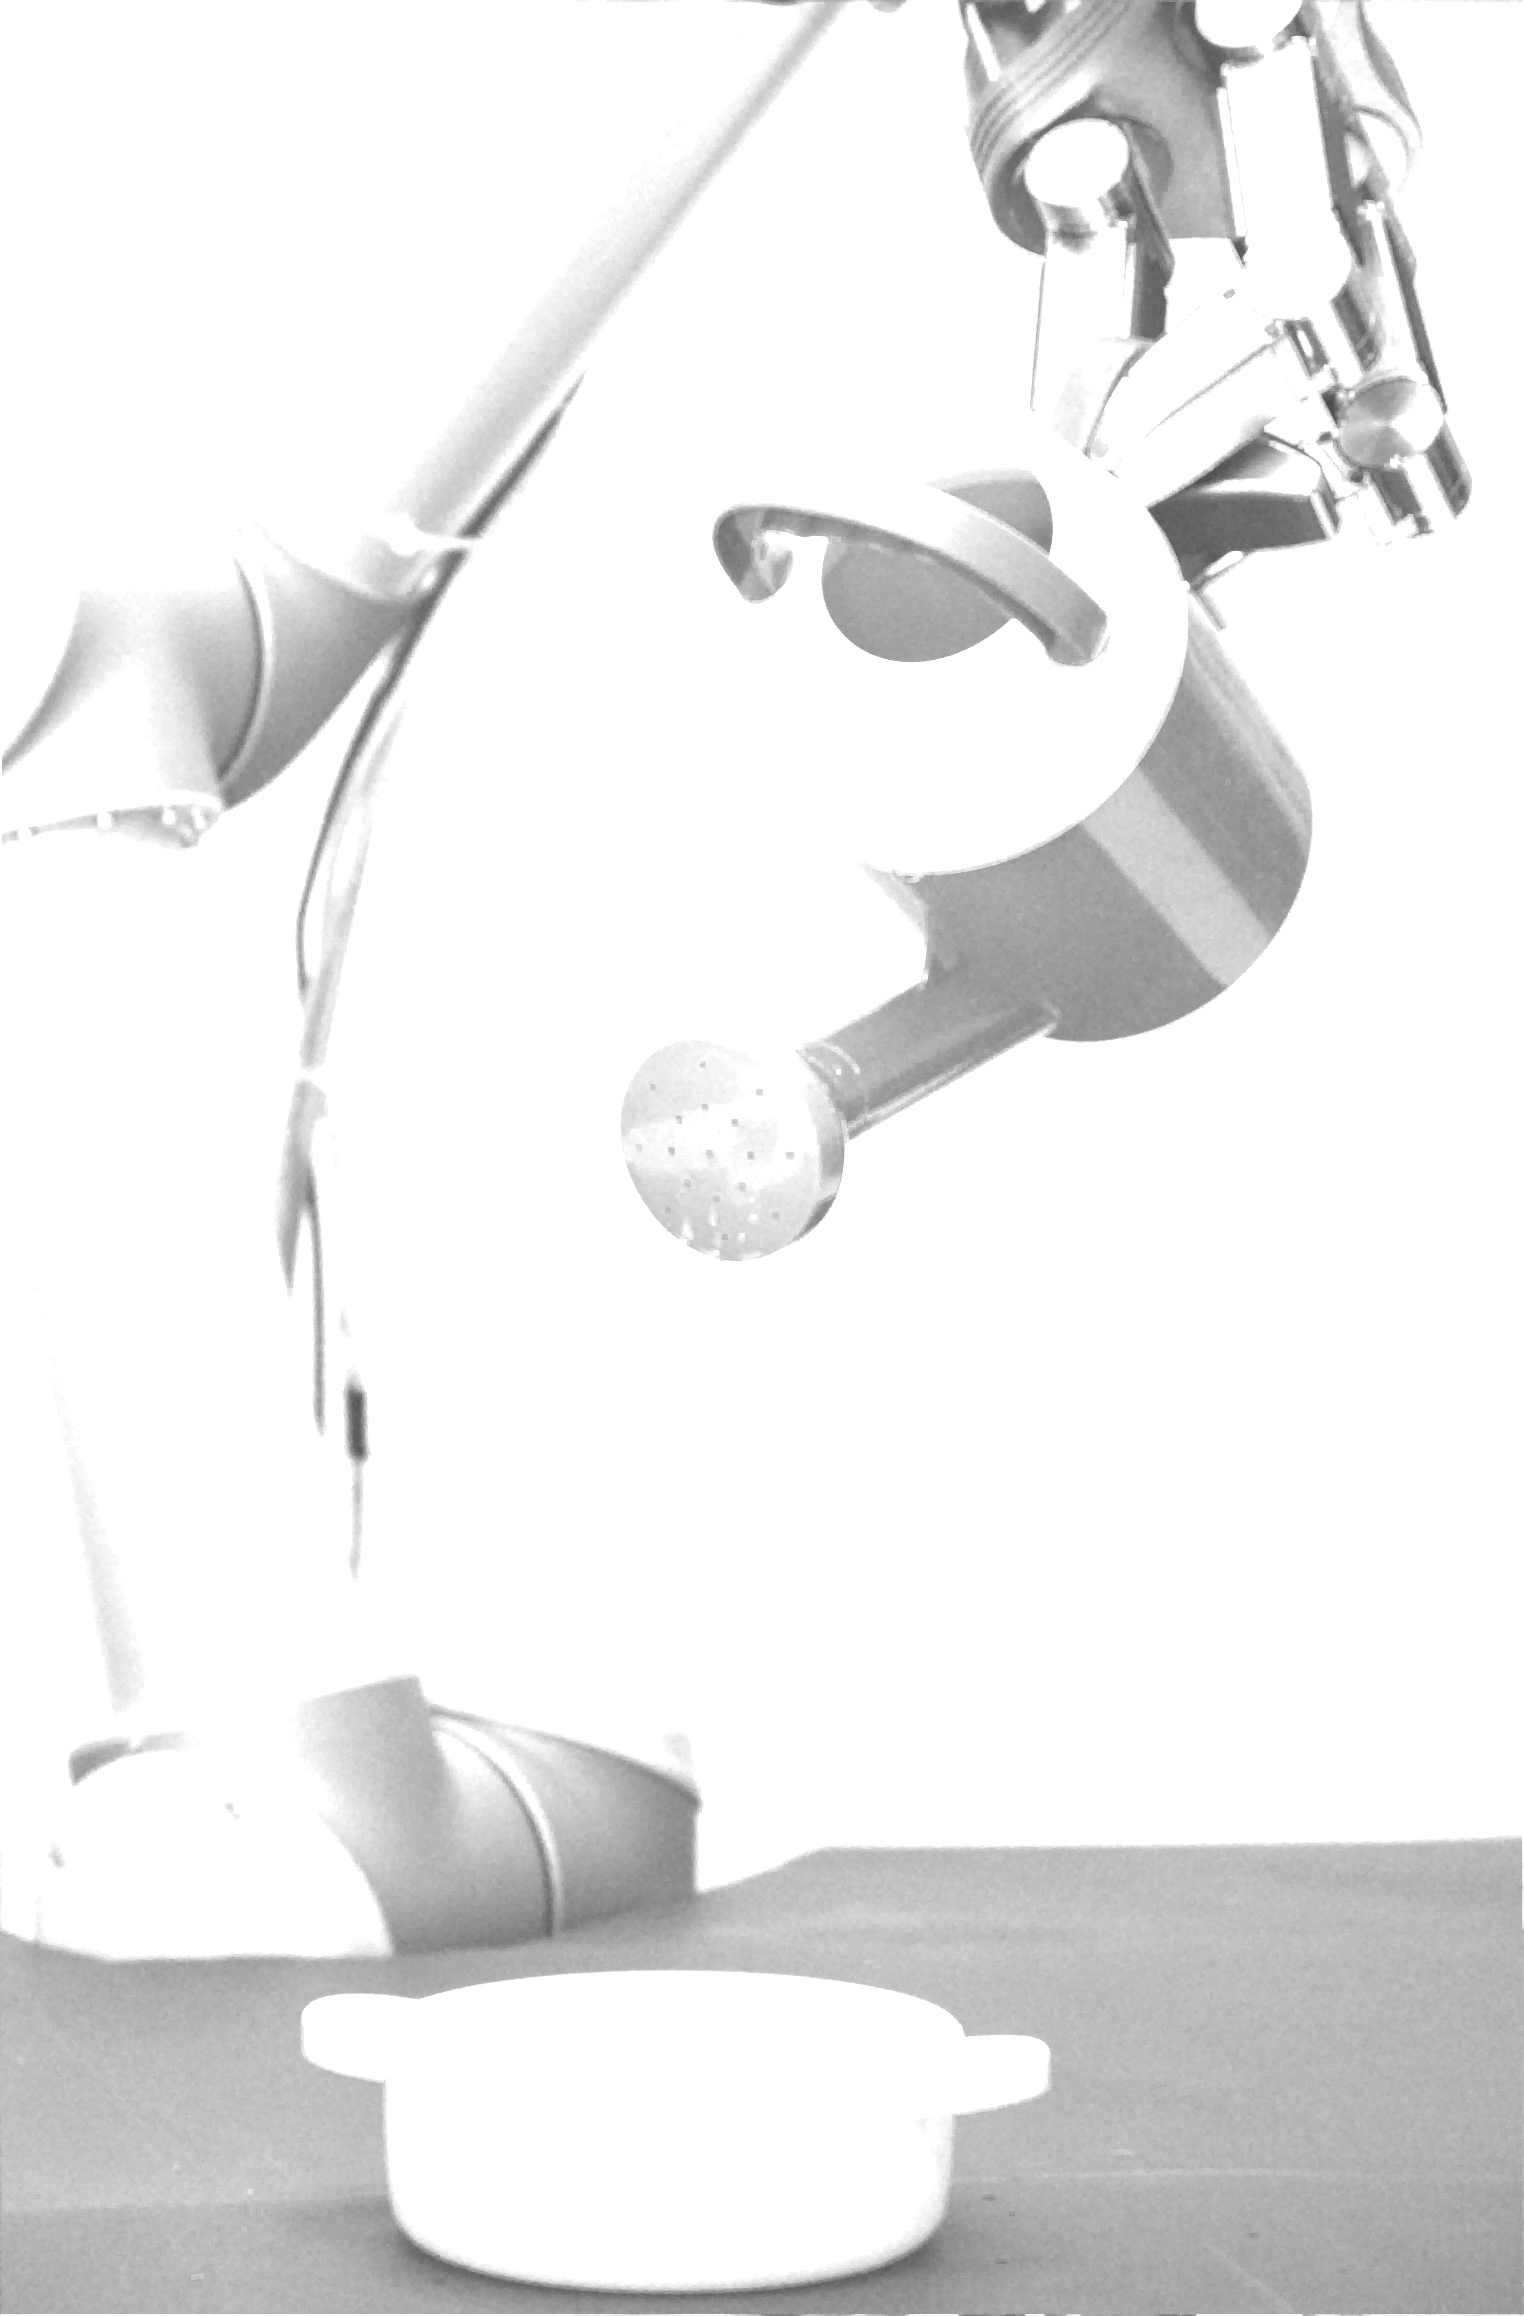
\includegraphics[width=\textwidth]{img3/test/contrast_5_1_7_final_img3.png}
    \end{subfigure}
        \begin{subfigure}[b]{0.1\textwidth}
        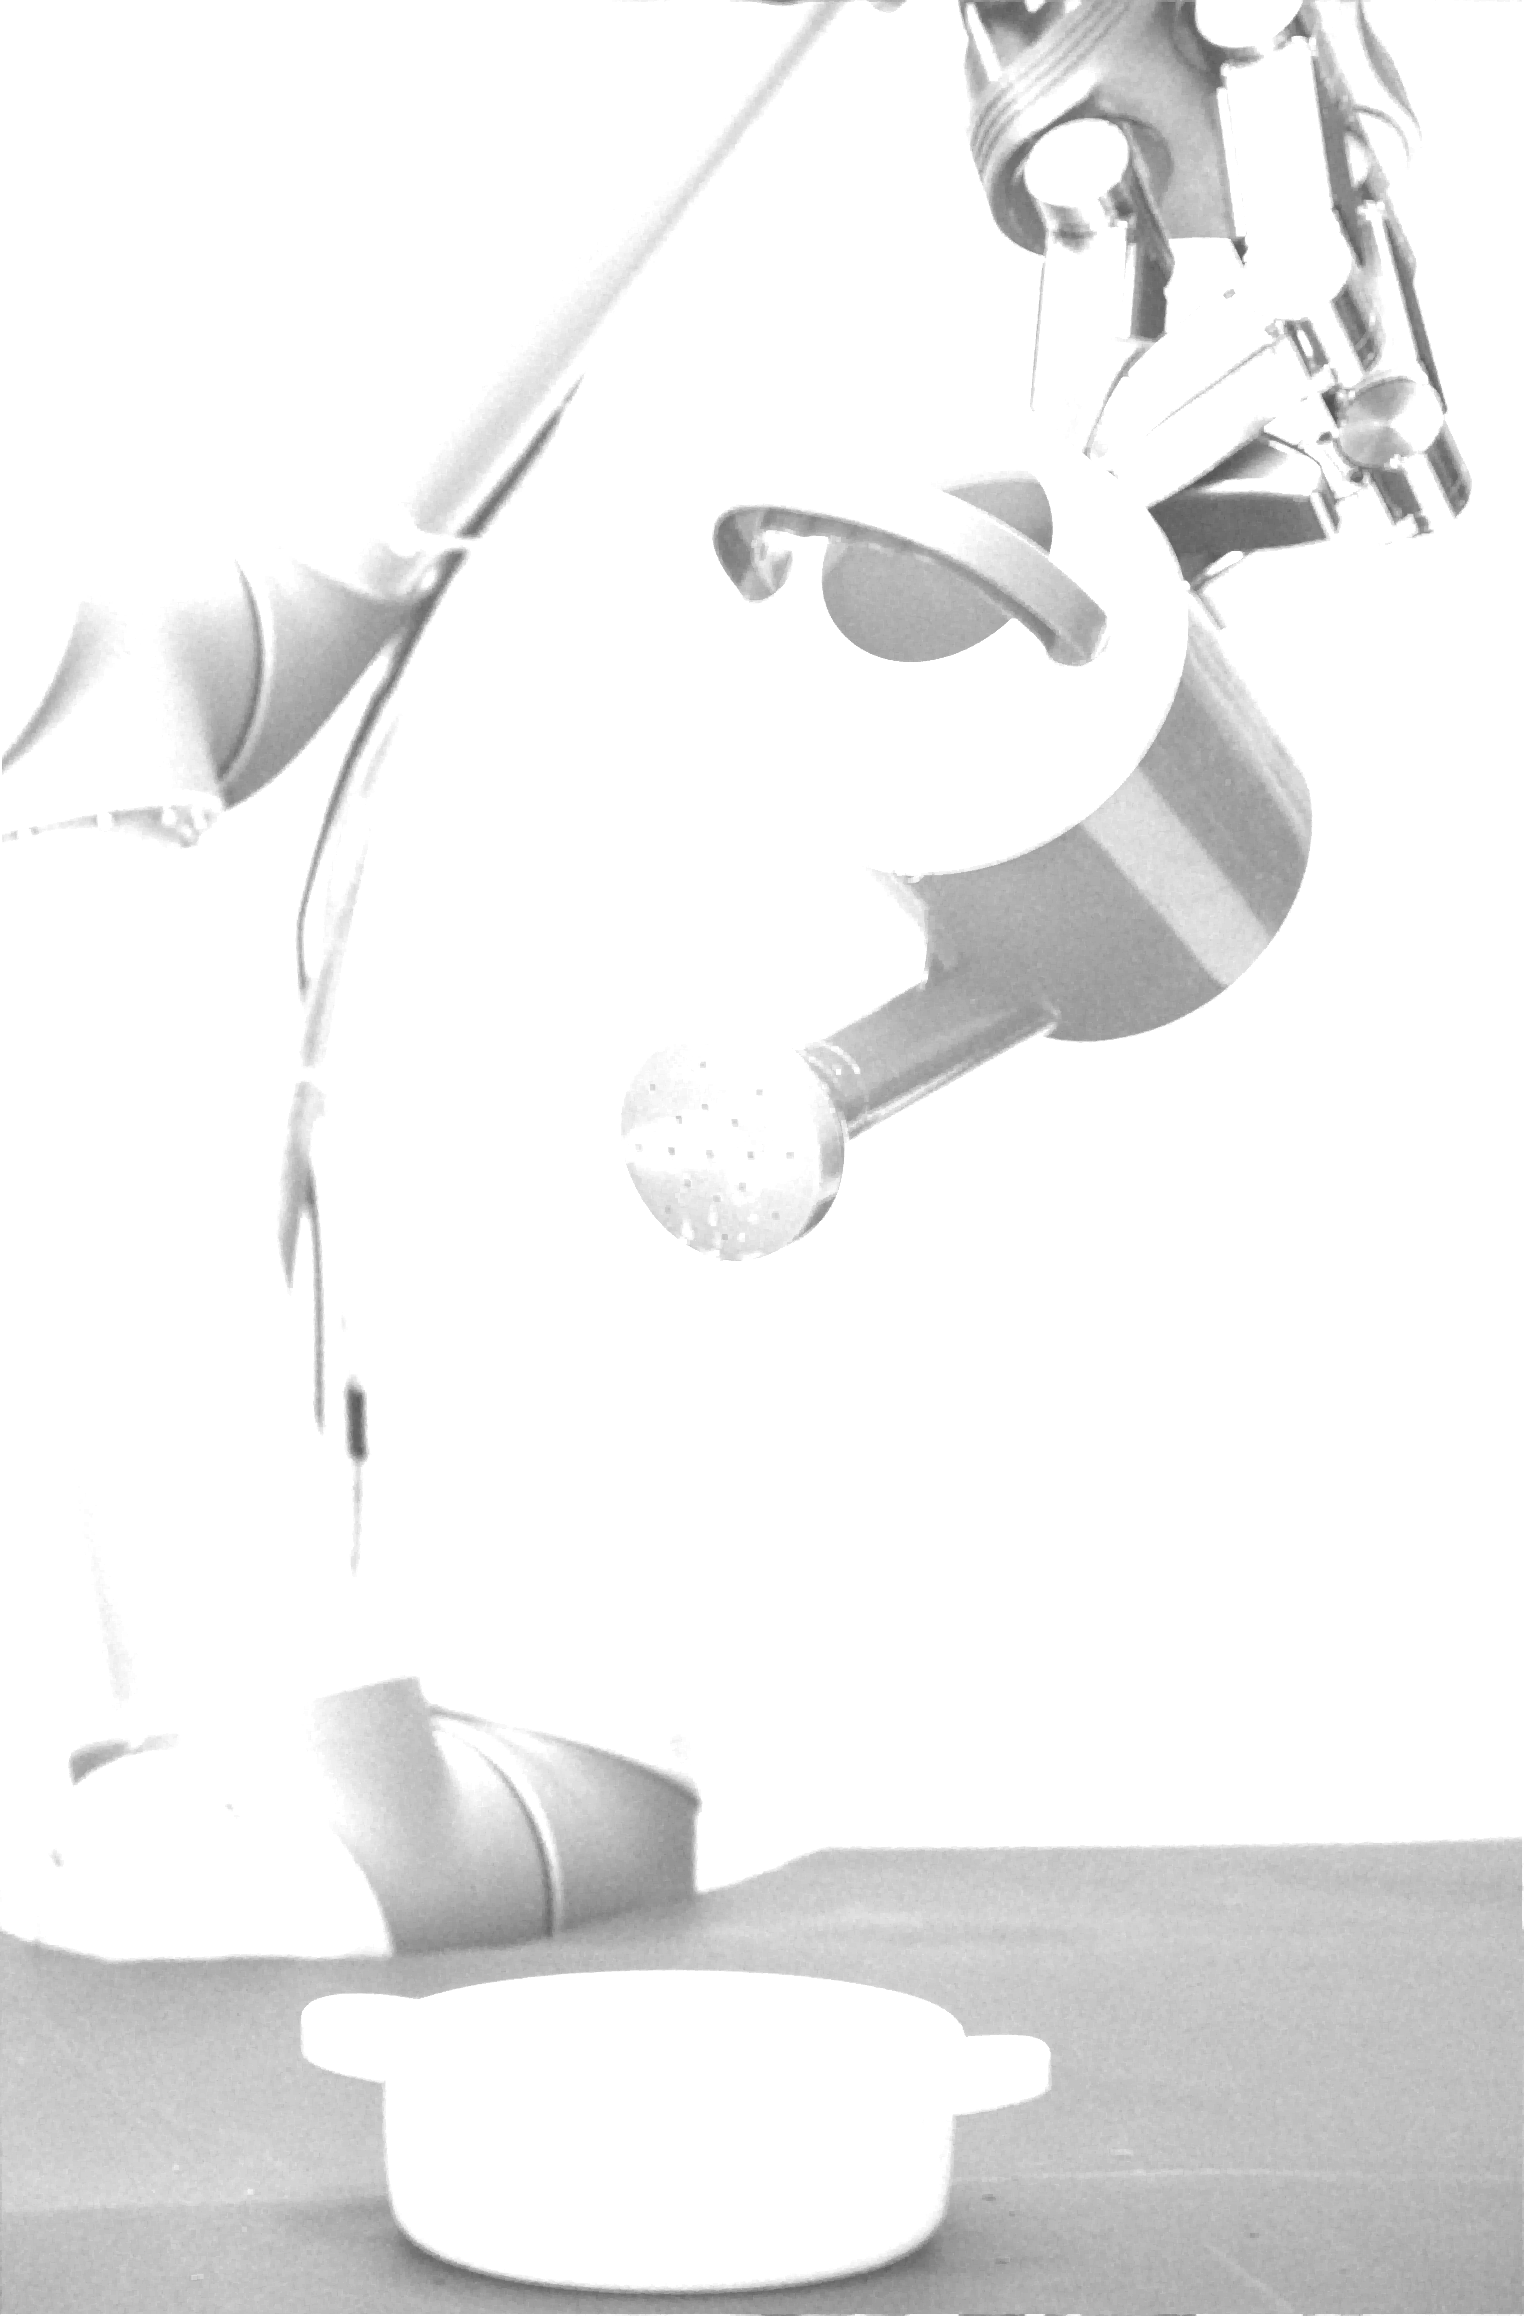
\includegraphics[width=\textwidth]{img3/test/contrast_5_1_8_final_img3.png}
    \end{subfigure}
        \begin{subfigure}[b]{0.1\textwidth}
        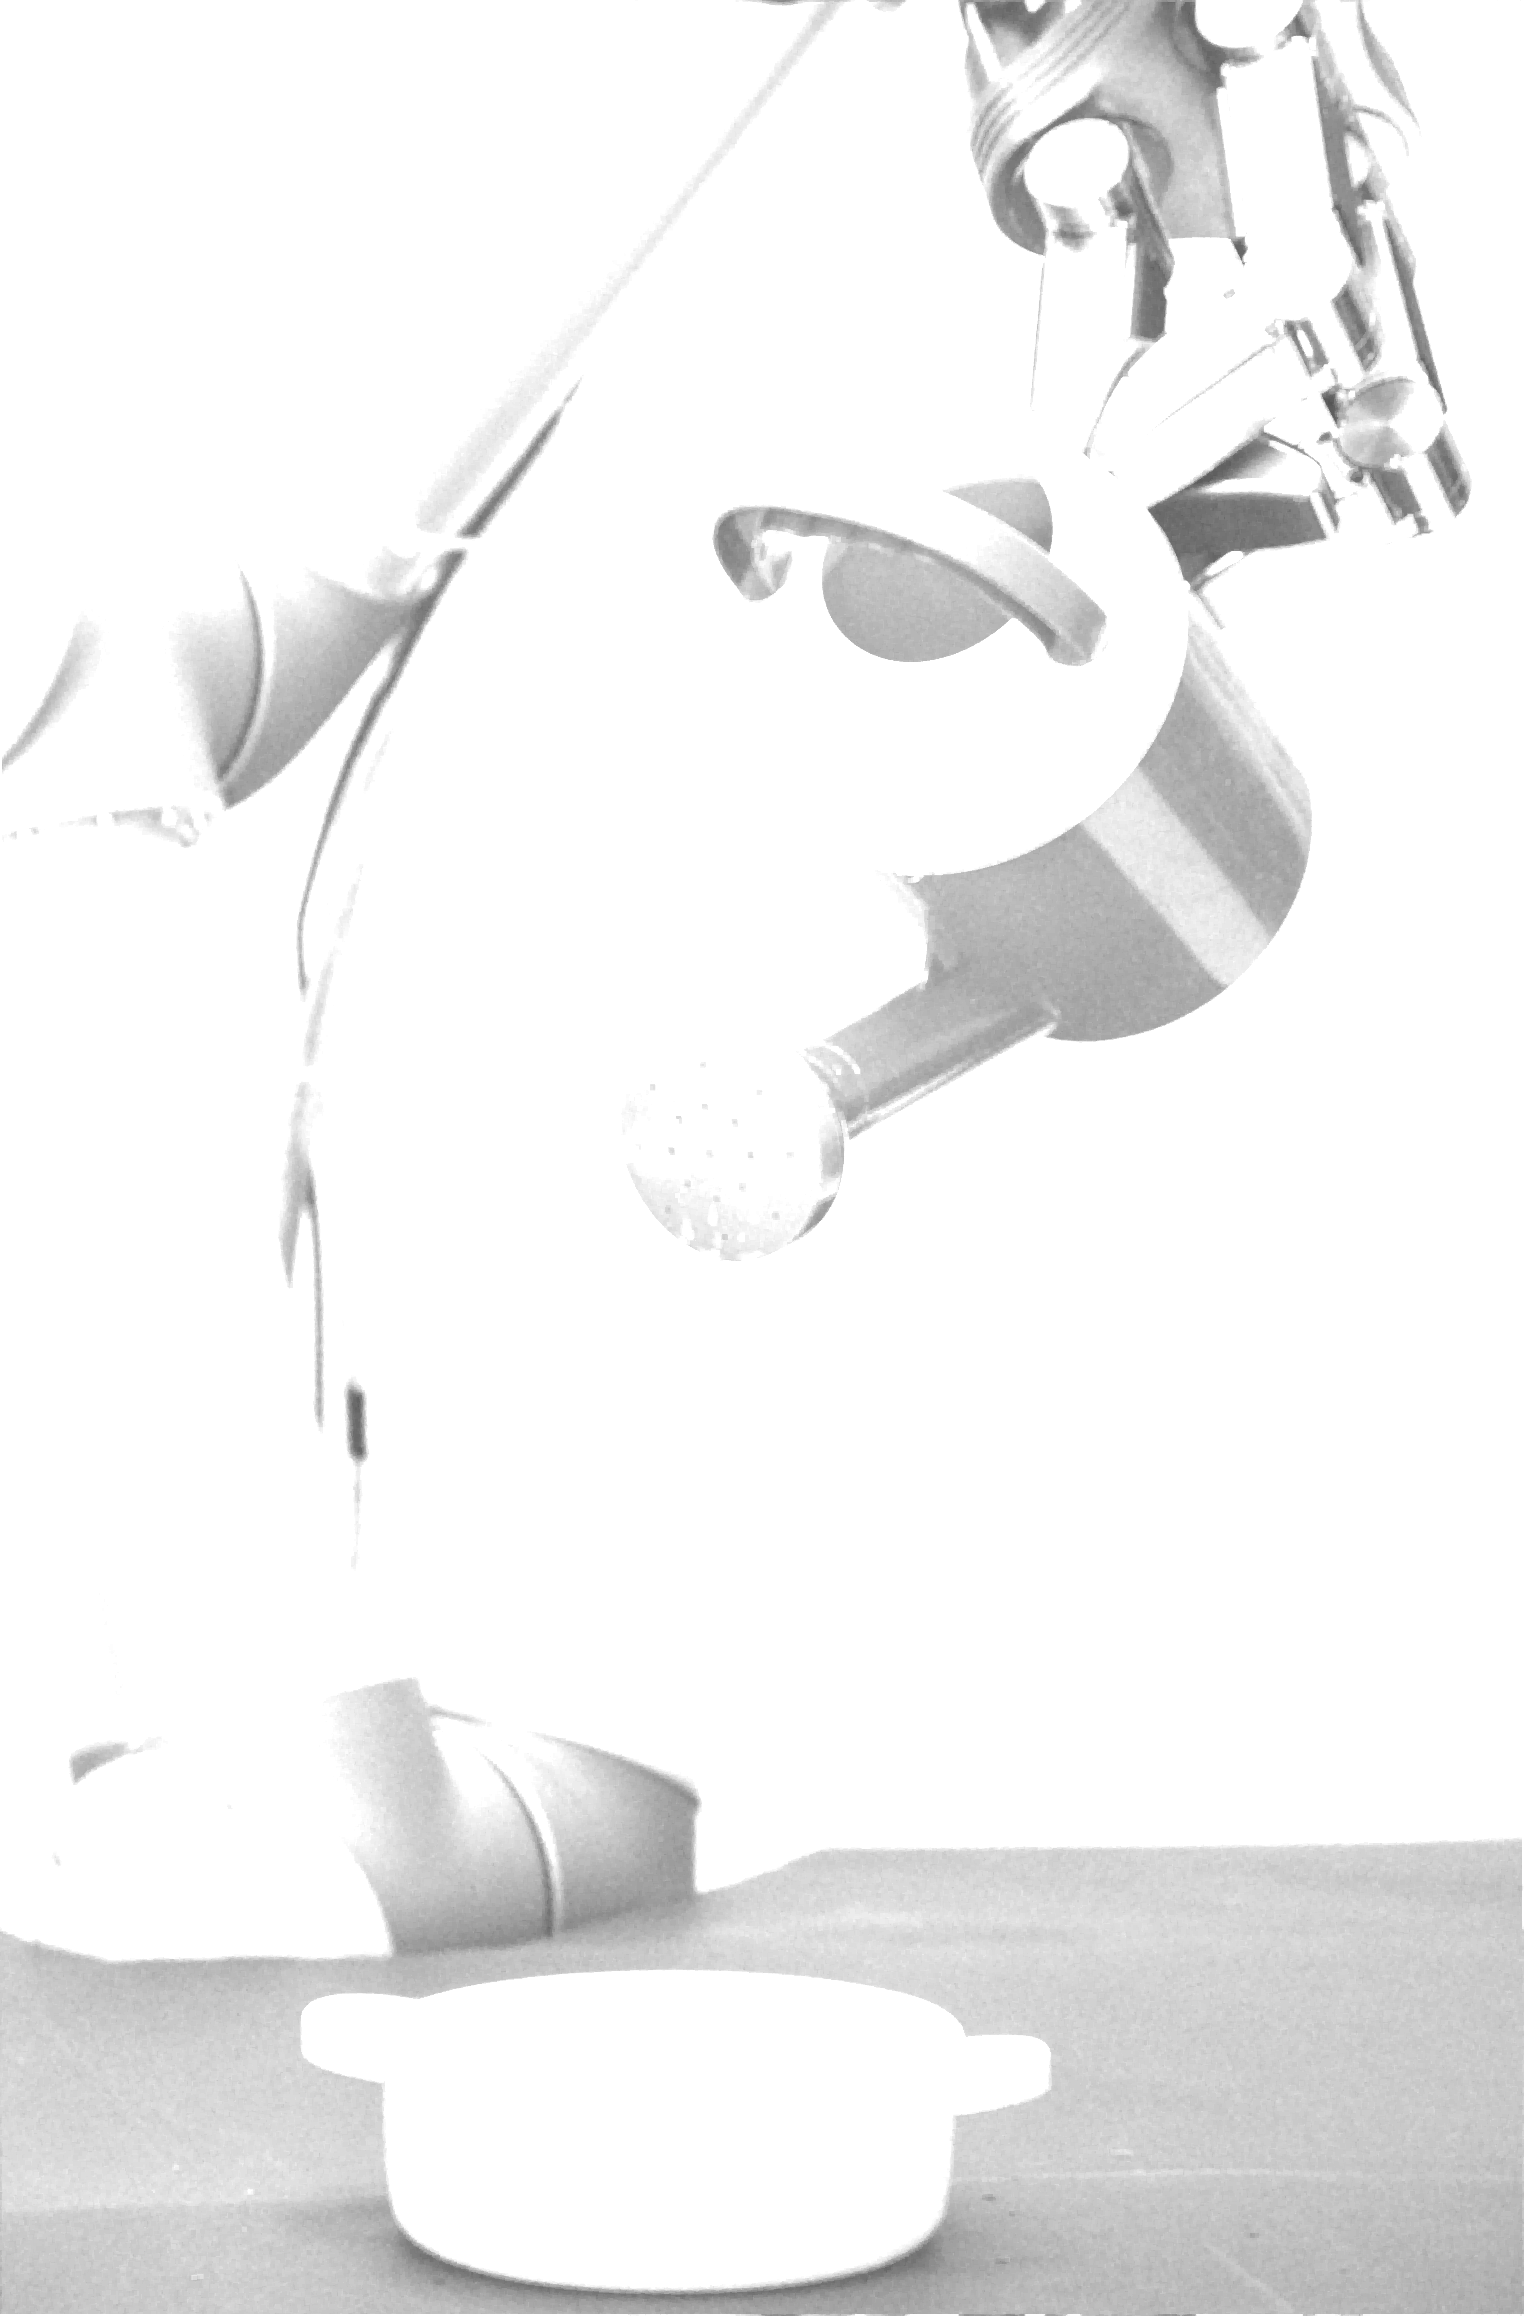
\includegraphics[width=\textwidth]{img3/test/contrast_5_1_9_final_img3.png}
    \end{subfigure}
    \caption{Testing for the right brightness}
    \label{fig:img3_test_brightness}
\end{figure} 

\begin{figure}[H]
    \centering
    \begin{subfigure}[b]{0.28\textwidth}
        \includegraphics[width=\textwidth]{img3/midpoint_5_final_img3.png}\\[0.1cm]
        \includegraphics[width=\textwidth]{img3/hist_rect_5_midpoint_5_final_img3_org.png}
        \begin{center}
        	\textbf{Uniform surfaces}
        \end{center}
        \includegraphics[width=\textwidth]{img3/rect_5_midpoint_5_final_img3.png}\\[0.1cm]
        \includegraphics[width=\textwidth]{img3/hist_rect_5_midpoint_5_final_img3.png}
        \caption{Kernel 5}
        \label{fig:img3_kernel_5_final}
    \end{subfigure}
    \begin{subfigure}[b]{0.28\textwidth}
        \includegraphics[width=\textwidth]{org.png}\\[0.1cm]
        \includegraphics[width=\textwidth]{img2/hist_eee_org_res_total.png}
        \begin{center}
        	\text{ }
        \end{center}
        \includegraphics[width=\textwidth]{img2/rect_eee_org_res_total.png}\\[0.1cm]
        \includegraphics[width=\textwidth]{img2/hist_rect_eee_org_res_total.png}
        \caption{Original}
        \label{fig:img3_org_final}
    \end{subfigure}
    \begin{subfigure}[b]{0.28\textwidth}
        \includegraphics[width=\textwidth]{img3/contrast_5_0_85_final_img3.png}\\[0.1cm]
        \includegraphics[width=\textwidth]{img3/hist_0_85_contrast_5_0_85_final_img3.png}
        \begin{center}
        	\text{ }
        \end{center}
        \includegraphics[width=\textwidth]{img3/rect_0_85_contrast_5_0_85_final_img3.png}\\[0.1cm]
        \includegraphics[width=\textwidth]{img3/hist_rect_0_85_contrast_5_0_85_final_img3.png}
        \caption{\lstinline|converTo| with 0.85}
        \label{fig:img3_contrast}
    \end{subfigure}
    \caption{Examples of different noise models}
    \label{fig:noise_examples_img3}
\end{figure} 

\todo{lidt forvirret omkring konklussionen.. hvad er dit endelig svar?}


\section{Image 4}
Figure \ref{fig:img42_src} shows  Image4\_2 which has to be restored. This image  compared to the original  (Figure \ref{fig:orignal}) has some both horizontal and vertical stripes.   Based on the frequency spectrum of this image, it can be seen that some frequency component exist around the center frequency creating this effect. The purpose of this restoration will be to reduce the effect of these component, and reconstruct it so it resembles Figure \ref{fig:orignal}

\begin{figure}[H]
    \centering
    \begin{subfigure}[b]{0.23\textwidth}
        \includegraphics[width=\textwidth]{img4/Image4_2.png}
        \caption{Image4\_2 with \\no restoration}
        \label{fig:img42_src}
    \end{subfigure}
    \begin{subfigure}[b]{0.23\textwidth}
        \includegraphics[width=\textwidth]{img4/Image4_2_freq_spec.png}
        \caption{Frequency spectrum of Image4\_2}
        \label{fig:img1_hist}
    \end{subfigure}
    \caption{Analysis of image 1}\label{fig:img1}
\end{figure}

The frequency components creating the circle are reason why the the stripes are occuring in the image.  One way of resolving this issue is to create a low pass filter, which let everything below a certain frequency pass, and the filter frequencies above away. \\

One type of lowpass filter is the butterworth lowpass filter which is defined as
\begin{equation}
	H(u,v) = \frac{1}{1+[\frac{D(u,v)}{D_0}]^{2n}}
	\label{eq:LBP}
	\cite{Bogen side 295}
\end{equation}
\todo{Cite til bogen side 295}
$D_0$ is the cutoff frequency given as the distance from the origin, n  is the order,  and D(u,v) is distance between a point (u,v) in the frequency domain and the center frequency rectangle, it is calculated as such. 

\begin{equation}
D(u,v) = [(u-P/2)^2 + (v-Q/2)^2]^{\frac{1}{2}} 
\end{equation}

P and Q is the padded size of the rectangle. \\


The cutoff frequency can easily by found, by computing the distance between the origin and the corresponding frequency component. The origin i as the pixel position $(1536 ,2408)$, and one of the undesired frequency component lies as pixel position $(2336,2400)$ \\


This distance is computed to be 800, which means that $D_0$ below 800, should be able to filter out the frequency components causing the stripes. \\

\begin{figure}[H]
    \centering
    \begin{subfigure}[b]{0.16\textwidth}
        \includegraphics[width=\textwidth]{img2/src.png}
        \caption{The original image}
        \label{fig:img2_src}
    \end{subfigure}
    \begin{subfigure}[b]{0.16\textwidth}
        \includegraphics[width=\textwidth]{img2/hist.png}
        \caption{Histogram of the original image}
        \label{fig:img2_hist}
    \end{subfigure}
	 \begin{subfigure}[b]{0.16\textwidth}
        \includegraphics[width=\textwidth]{img2/src.png}
        \caption{The original image}
        \label{fig:img2_src}
    \end{subfigure}
    \begin{subfigure}[b]{0.16\textwidth}
        \includegraphics[width=\textwidth]{img2/hist.png}
        \caption{Histogram of the original image}
        \label{fig:img2_hist}
    \end{subfigure}	
\begin{subfigure}[b]{0.16\textwidth}
        \includegraphics[width=\textwidth]{img2/src.png}
        \caption{The original image}
        \label{fig:img2_src}
    \end{subfigure}
    \begin{subfigure}[b]{0.16\textwidth}
        \includegraphics[width=\textwidth]{img2/hist.png}
        \caption{Histogram of the original image}
        \label{fig:img2_hist}
    \end{subfigure}	
    
    
      \begin{subfigure}[b]{0.16\textwidth}
        \includegraphics[width=\textwidth]{img2/src.png}
        \caption{The original image}
        \label{fig:img2_src}
    \end{subfigure}
    \begin{subfigure}[b]{0.16\textwidth}
        \includegraphics[width=\textwidth]{img2/hist.png}
        \caption{Histogram of the original image}
        \label{fig:img2_hist}
    \end{subfigure}
	 \begin{subfigure}[b]{0.16\textwidth}
        \includegraphics[width=\textwidth]{img2/src.png}
        \caption{The original image}
        \label{fig:img2_src}
    \end{subfigure}
    \begin{subfigure}[b]{0.16\textwidth}
        \includegraphics[width=\textwidth]{img2/hist.png}
        \caption{Histogram of the original image}
        \label{fig:img2_hist}
    \end{subfigure}	
\begin{subfigure}[b]{0.16\textwidth}
        \includegraphics[width=\textwidth]{img2/src.png}
        \caption{The original image}
        \label{fig:img2_src}
    \end{subfigure}
    \begin{subfigure}[b]{0.16\textwidth}
        \includegraphics[width=\textwidth]{img2/hist.png}
        \caption{Histogram of the original image}
        \label{fig:img2_hist}
    \end{subfigure}
    
    
      \begin{subfigure}[b]{0.16\textwidth}
        \includegraphics[width=\textwidth]{img2/src.png}
        \caption{The original image}
        \label{fig:img2_src}
    \end{subfigure}
    \begin{subfigure}[b]{0.16\textwidth}
        \includegraphics[width=\textwidth]{img2/hist.png}
        \caption{Histogram of the original image}
        \label{fig:img2_hist}
    \end{subfigure}
	 \begin{subfigure}[b]{0.16\textwidth}
        \includegraphics[width=\textwidth]{img2/src.png}
        \caption{The original image}
        \label{fig:img2_src}
    \end{subfigure}
    \begin{subfigure}[b]{0.16\textwidth}
        \includegraphics[width=\textwidth]{img2/hist.png}
        \caption{Histogram of the original image}
        \label{fig:img2_hist}
    \end{subfigure}	
\begin{subfigure}[b]{0.16\textwidth}
        \includegraphics[width=\textwidth]{img2/src.png}
        \caption{The original image}
        \label{fig:img2_src}
    \end{subfigure}
    \begin{subfigure}[b]{0.16\textwidth}
        \includegraphics[width=\textwidth]{img2/hist.png}
        \caption{Histogram of the original image}
        \label{fig:img2_hist}
    \end{subfigure}
\end{figure}


From the figure (comming) it can be seen that the filters weakens the effect of the frequency components. Some ringing effect occurs as the image gets filtered with higher order filter. This is due to the transition occuring more abruptly thus resembling the an ideal filter. 

\begin{figure}[H]
	\centering
	\includegraphics[width=0.3\textwidth]{img4/filter_become_ideal2.png}
	\caption{Filter becomes more ideal as the order increases.}
    \label{fig:filter_become_ideal}
\end{figure}


The image which was used for further processing is the output generated by applying a low pass buterworth filter with an $d_0 = 650$ and order of 9. \\
 
 By resembling the output from the filter with original it can be see that the constrast differs a bit compared with the original,  hence contrast streching be applied on to the image, which returns this image. 
 
 \begin{figure}[H]
 \centering
 \includegraphics[width=0.3\textwidth]{img4/filteredOutput_6509_contrast_strech.png}
 	\caption{Contrast strecthing applied to the image. }
    \label{fig:filter_become_ideal}
\end{figure} 

At this point it was determined that the image was restored enough, to resemble the original image. 

\begin{figure}[H]
\centering
    \begin{subfigure}[b]{0.24\textwidth}
        \includegraphics[width=\textwidth]{img4/Image4_2.png}
        \caption{Start image}
        \label{fig:img2_hist}
    \end{subfigure}
	 \begin{subfigure}[b]{0.24\textwidth}
        \includegraphics[width=\textwidth]{img4/Image4_2.png}
        \caption{Lowpass filtered}
        \label{fig:img2_src}
    \end{subfigure}
    \begin{subfigure}[b]{0.24\textwidth}
        \includegraphics[width=\textwidth]{img4/filteredOutput_6509_contrast_strech.png}
        \caption{Contrast stretched}
        \label{fig:img2_hist}
    \end{subfigure}	
\begin{subfigure}[b]{0.24\textwidth}
        \includegraphics[width=\textwidth]{org.png}
        \caption{The original image}
        \label{fig:img2_src}
    \end{subfigure}
\end{figure}





\section{Image 5}
\input{img5.tex}





\end{document}






















































